\documentclass[a4paper]{article}

\author{Misrraim~Su\'arez~P\'erez}
\title{FirstMarket}



\usepackage[utf8]{inputenc}
\usepackage[spanish,es-tabla,es-nodecimaldot,es-lcroman]{babel}

\usepackage{csquotes}
\linespread{1.25}

\usepackage{graphicx}
\graphicspath{ {./images/} }

\usepackage{xcolor}

\usepackage{listings}
\lstdefinelanguage{JavaScript}{
	keywords={typeof, new, true, false, catch, function, return, null, catch, switch, var, if, in, while, do, else, case, break, let, const},
	keywordstyle=\color{blue}\bfseries,
	ndkeywords={class, export, boolean, throw, implements, import, this},
	ndkeywordstyle=\color{darkgray}\bfseries,
	identifierstyle=\color{black},
	sensitive=false,
	comment=[l]{//},
	morecomment=[s]{/*}{*/},
	commentstyle=\color{purple}\ttfamily,
	stringstyle=\color{olive}\ttfamily,
	morestring=[b]',
	morestring=[b]"
}
\lstset{
	language=JavaScript,
	backgroundcolor=\color{lightgray},
	extendedchars=true,
	basicstyle=\footnotesize\ttfamily,
	showstringspaces=false,
	showspaces=false,
	numbers=left,
	numberstyle=\footnotesize,
	numbersep=9pt,
	tabsize=2,
	breaklines=true,
	showtabs=false,
	captionpos=b
}


\usepackage{hyperref}
\hypersetup{
	colorlinks=true,
	linkcolor=blue,
	filecolor=magenta,      
	urlcolor=cyan,
}

\urlstyle{same}

%\setcounter{tocdepth}{4}

%\setcounter{secnumdepth}{4}


\begin{document}

    \maketitle
    \tableofcontents

    \section{Introducción}
    El presente proyecto se enmarca dentro del Proyecto Final de Grado correspondiente al Grado en Ingeniería Informática de la Universidad Nacional de Educación a Distancia.
    
    Se basa en el proyecto específico ofertado por el Departamento de Sistemas de Comunicación y Control de la UNED titulado \emph{Desarrollo de un portal de comercio electrónico}. Citando la propia descripción de dicha oferta de proyecto específico:
    
    \begin{displayquote}
        El proyecto consiste en el desarrollo de un portal web orientado al comercio electrónico. Dicha aplicación permitirá al comprador seleccionar artículos, realizar pedidos y pagos a través de una pasarela. El sistema también ofrecerá al comerciante gestionar los artículos expuestos en el portal.
    \end{displayquote}

	En este contexto, el comercio electrónico desarrollado a sido una librería, denominada \textbf{FirstMarket}.

    \subsection{Motivación y Objetivos}
    Desde un primer momento la intención fue desarrollar un proyecto que tuviese la mayor relación posible con el mercado actual, lo que, junto con un fuerte interés personal hacia el ecosistema de Internet, llevó a la decisión de escoger esta propuesta.
    
    La idea era desarrollar algo moderno, útil, con reflejo real en la sociedad y que cumpliese el papel de facilitar la inserción laboral. En este sentido, las aplicaciones web en general, y las específicas de comercio electrónico en particular, cumplen a la perfección los requisitos comentados. A nadie se le escapa hoy en día la implantación casi ubicua que estas tecnologías tienen en la sociedad.
    
    Por otro lado, y en clara conexión con lo comentado, otro objetivo de este último trabajo del plan de estudios fue el de servir como \emph{compensador} final de lagunas formativas. En este sentido, el control de versiones con Git era una tarea pendiente inaplazable, así como profundizar en tecnologías web básicas como HTTP, HTML, CSS ó JavaScript. Además, ampliar el dominio de las tecnologías Java siempre fue algo muy deseable.
    
    Conviene no dejar de lado, por obvio, que un objetivo fundamental del presente trabajo es el de dar fin al plan de estudios. Remarcar esto es relevante porque en múltiples situaciones puede entrar en conflicto con la intención de desarrollar una aplicación web lo más moderna posible. Como se explicará más adelante en esta memoria, el mundo de las tecnologías web es muy cambiante, y pretender desarrollar una aplicación web alineada con el estado del arte en la materia partiendo, como es el caso, desde prácticamente cero conocimientos, sale fuera del marco de un trabajo de estas características. Por tanto, siempre se ha tenido en cuenta un compromiso entre recursos disponibles (principalmente tiempo y conocimientos) y grado de modernidad en las tecnologías usadas.
    \\
    
    En definitiva, el principio fundamental que ha guiado la toma de decisión ha sido el reforzar, y alinear en la medida de lo posible con el estado del arte, las habilidades técnicas adquiridas fruto del plan de estudios, de forma a facilitar una futura integración en la industria web, a la par de satisfacer una histórica inquietud personal en la materia.


    \subsection{Internet, Web y Aplicaciones Web}
    En esta sección se ofrece una introducción, meramente descriptiva, del contexto en el que situar la aplicación web desarrollada. Se tratará de diferenciar los conceptos de Internet, World Wide Web y aplicaciones web.

    \subsubsection{¿Qué es Internet?}
    Tal como se explica en [bib ref], esta pregunta puede ser enfocada desde dos puntos de vista complementarios.
    
    Por un lado, desde una perspectiva \textbf{hardware}, Internet es una red que conecta miles de millones de dispositivos en todo el mundo, denominados \emph{hosts} o \emph{sistemas finales}, por medio de \emph{enlaces de comunicación} y \emph{conmutadores de paquetes}.
    
    Los enlaces de comunicación son diferentes tipos de medios físicos a través de los cuales se transfieren ondas electromagnéticas que portan la información. Puede tratarse de medios guiados, como cables de cobre, cables coaxiales o fibra óptica, o no guiados, como el espectro de radio. Cuando un sistema final decide enviar información a otro sistema final, el emisor fragmenta los datos en \emph{paquetes} de información y los envía al destinatario a través de la red. Una vez en destino, el sistema final receptor ensambla los paquetes para reconstruir los datos originales. Un conmutador de paquetes toma un paquete que llega a uno de sus enlaces de comunicación entrantes y decide hacia cuál de sus enlaces de comunicación salientes lo reenvía.
    
    Estas \emph{redes de conmutación de paquetes} se pueden entender de forma análoga a una empresa que necesita mover una gran cantidad de carga entre dos almacenes separados gran distancia. En el almacén de origen la carga se divide y organiza en diferentes contenedores. Cada uno de los contenedores viaja de forma independiente a través de la red de transporte disponible siguiendo posiblemente rutas no del todo iguales. Por ejemplo, unos contenedores pueden ir por ciertas carreteras en ciertos camiones mientras que otros pueden viajar en tren o incluso en barco, o cualquier combinación de los anteriores. Lo importante es la independencia entre la ruta de un contenedor concreto con los demás. Una vez llegados al almacén de destino, la carga se extrae de los contenedores y se agrupa con el resto que llega del mismo envío. Así, los paquetes son análogos a los contenedores, los enlaces de comunicación son análogos a las vías de transporte, los conmutadores de paquetes son análogos a las intersecciones o discontinuidades en las vías de transporte (piénsese en una simple rotonda), y los sistemas finales son análogos a los almacenes. Pues bien, de igual forma que un contenedor toma un camino a través de la red de transporte, un paquete de información toma un camino a través de la infraestructura de Internet.
    
    Por otro lado, es posible describir Internet desde un punto de vista \textbf{software} como un servicio prestado a las aplicaciones distribuidas, es decir, como una interfaz de programación que las aplicaciones distribuidas consumen.
    
    Se dice que las aplicaciones son aplicaciones distribuidas, o \textbf{aplicaciones de Internet}, cuando se ejecutan en diferentes máquinas que intercambian datos entre sí. Es importante destacar que las aplicaciones de Internet se ejecutan estrictamente en los sistemas finales, no en la infraestructura de la red, que es agnóstica (o debiera serlo) de la semántica de la información que está trasportando. Así, puede pensarse en Internet como un servicio postal, que garantiza el envío de información entre partes, las cuales pueden estar desarrollando cualquier tipo de actividad basada, entre otras cosas, en la propia comunicación que mantienen. Al igual que el servicio postal impone una serie de reglas para ser usado, como dónde depositar la carta que se pretende enviar o dónde y de qué manera especificar la dirección de envío, Internet ofrece unas reglas en forma de interfaz de programación que las aplicaciones de Internet deben adoptar.
    
    \subsubsection{¿Qué es la Web?}
    Siguiendo el hilo de la discusión del epígrafe anterior, la World Wide Web es una de las muchas aplicaciones de Internet existentes. Otras serían el correo electrónico, las aplicaciones para acceder remotamente a otra máquina, la transferencia de archivos, el streaming de video, la telefonía por Internet, y más.
    
    A veces, dado que la Web es la aplicación más conocida, se confunde la parte con el todo al identificarla con la propia Internet. Sin embargo, esta aplicación surgió bastante tiempo después de que otras ya estuvieran ampliamente implantadas y maduras, como el correo electrónico o la transferencia de ficheros, si bien su uso era principalmente en ámbitos académicos.
    
    Lo que da tanta importancia a la Web es que fue la aplicación de Internet que, a principios de los años 90, abrió al gran público a la hasta entonces desconocida Internet. De hecho, esta aplicación llevó a Internet de ser tan sólo una más de muchas redes existentes a ser la dominante por excelencia.
   
   	Entonces, como se ha dicho, la Web es una aplicación de Internet, y como tal se trata de software que se ejecuta en diferentes máquinas que intercambian mensajes entre sí. El formato de estos mensajes, su timing y demás \emph{reglas de conversación} se recogen en un protocolo, el HyperText Transfer Protocol (HTTP). Este protocolo es el corazón de la Web, encontrándose definido en [RFC 1945] y en [RFC 2616], y su implementación se materializa en dos programas ejecutados en diferentes sistemas finales, un programa cliente y un programa servidor.
    
    La mecánica básica gira en torno a peticiones y respuestas. El programa cliente envía un mensaje HTTP conteniendo una petición al programa servidor. Por su parte, siguiendo las reglas definidas en el protocolo, el programa servidor contesta enviando otro mensaje HTTP al cliente. En el caso más común, el cliente le solicita al servidor el envío de una \emph{página web}.
    
    Una página web es un documento de texto escrito con unas reglas de sintaxis específicas. Estas reglas definen el Hypertext Markup Language (HTML). En el sistema final cliente, la página web es presentada en pantalla de una manera amigable al usuario por medio de programas que procesan el contenido en HTML.
    
    En definitiva, y sin entrar en matices que desvíen de la esencia, la Web es la aplicación de Internet que permite el consumo de páginas web bajo demanda por parte de los usuarios (en contraste con el modelo broadcast, en el que se emite y el usuario sólo puede consumir lo emitido, como en la radio).
    
    \subsubsection{¿Qué es una Aplicación Web?}
    
    %A web application is defined as a hierarchy of directories and files in a standard layout. Such a hierarchy can be accessed in its "unpacked" form, where each directory and file exists in the filesystem separately, or in a "packed" form known as a Web ARchive, or WAR file. The former format is more useful during development, while the latter is used when you distribute your application to be installed.
    
    
    %The complete syntax and semantics for the deployment descriptor is defined in Chapter 13 of the Servlet API Specification, version 2.3.
    
    Las páginas web que son enviadas desde el servidor al cliente se dice que pueden ser estáticas o dinámicas. Esta característica, más que hablar de la página web en sí misma, habla del proceso mediante el cual su contenido ha sido creado y modificado a lo largo del tiempo.
   	
   	Las páginas estáticas lo son en el sentido de que su contenido, creado comúnmente por un humano, no varía con el tiempo de manera programática. La información que presentan es la misma, a menos que se modifique \emph{a mano}. Así eran todas las páginas web en los primeros años. En contraste, en las páginas web dinámicas, el contenido no está dado de antemano, sino que se genera en cada ciclo de petición-respuesta. Esto es útil porque entre otras cosas permite páginas web personalizadas para cada usuario, e incluso que sea él mismo quien aporte contenido a la página web.
    
    Una \textbf{aplicación web} es el sistema software encargado de la generación dinámica de páginas webs. Normalmente, y a diferencia del modelo estático, entre sus componentes se encuentra una base de datos que permita la persistencia de la información, cambiante por definición de la propia arquitectura.
    
    Desde este punto de vista, en el presente proyecto se ha desarrollado una aplicación web encargada de generar contenido web que los usuarios pueden visitar con el objetivo de comprar libros a través de Internet.

    \subsection{Estructura de la Memoria}
    Estructura

    \section{Análisis}
        \subsection{Requisitos}
            La aplicación debe admitir los roles y capacidades siguientes:
            \begin{enumerate}
                \item Usuario anónimo (UA).
                \begin{itemize}
                    \item[-] Por defecto, al acceder al sitio web se hace como UA, sin ninguna validación ni credencial. Basta con acceder a la URL de inicio de la aplicación.
                    \item[-] Un UA debe poder realizar búsquedas de libros, es decir, debe tener pleno acceso a la exploración del catálogo.
                    \item[-] La plena exploración del catálogo debe permitir realizar búsque\-das filtradas según 0, 1 o más criterios, tales como: categoría, título o autor.
                    \item[-] Un UA debe poder visualizar información detallada de un libro, por ejemplo de entre los obtenidos tras una búsqueda.
                    \item[-] Un UA debe poder consultar las promociones disponibles.
                    \item[-] Un UA debe poder registrarse en el sistema completando un formulario (nombre, contraseña, dirección de correo electrónico, etc.).
                    \item[-] Finalizado el proceso de registro, el nuevo UR debe recibir confirmación por correo electrónico.
                    \item[-] En su caso, un UA debe poder iniciar sesión en el sistema.
                    \item[-] En su caso, un UA debe poder realizar el procedimiento de recuperación de contraseña.
                \end{itemize}
                \item Usuario registrado (UR). Este perfil representa a un usuario que ha pasado de anónimo a registrado. Un UR posee todas las capacidades del UA, más otras específicas suyas, a saber:
                \begin{itemize}
                    \item[-] Poder editar la información de su perfil de usuario.
                    \item[-] Realizar pedidos y efectuar los correspondientes pagos a través de una pasarela segura.
                    \item[-] Disponer de una cesta virtual para la gestión de la compra.
                    \item[-] En la cesta se debe poder introducir, modificar la cantidad o eliminar libros (esto último de uno en uno o todos a la vez).
                    \item[-] En cualquier momento del proceso de realizar un pedido, el UR debe poder cancelarlo.
                    \item[-] Tras una compra, el UR debe recibir confirmación en su correo electrónico.
                    \item[-] Un UR debe poder consultar el estado de sus pedidos.
                    \item[-] Puntuar (de alguna manera, p.e. estrellas del 1 al 5) un determinado libro que haya adquirido. Debe poder hacerlo en cualquier momento tras la compra.
                    \item[-] Consultar un histórico de sus transacciones, detallando los libros comprados, la fecha de la compra y el precio de cada uno.
                    \item[-] Darse de baja como UR.
                    \item[-] Cerrar sesión.
                    \item[-] Un UR debe poder ponerse en contacto con el administrador de la aplicación web a través de un formulario de contacto, recibiendo confirmación por correo electrónico tras el envío del mismo.
                \end{itemize}
                \item Usuario Administrador
                \begin{itemize}
                    \item[-] Ver y editar (añadir, modificar, eliminar) la jerarquía de categorías (CRUD categorías).
                    \item[-] Ver y editar (añadir, modificar, eliminar) la información relativa a los libros (título, autor/es, editorial, precio, disponibilidad, \ldots) (CRUD libros).
                    \item[-] Crear, modificar o eliminar promociones de libros (CRUD promociones).
                    \item[-] Tener acceso a la información de los UR, salvo sus contraseñas.
                    \item[-] Bloquear-desbloquear a un UR.
                    \item[-] Visualizar la información de los pedidos, tanto los que estén en curso como los finalizados.
                    \item[-] Poder alterar el estado de un pedido.
                    \item[-] Poder generar informes (p.e. ventas durante un determinado periodo con su importe y la facturación total).
                \end{itemize}
            \end{enumerate}

            Además de lo anterior, la aplicación debe:
            \begin{enumerate}
                \item[a)] Garantizar la persistencia de los datos referentes a UR, pedidos, pagos, productos y sus categorías.
                \item[b)] Mostrar un mensaje de error cuando un usuario introduzca incorrectamente sus credenciales de autenticación.
            \end{enumerate}

        \subsection{Casos de Uso}
            En este apartado se presentan las interacciones más comunes que los usuarios pueden realizar con la aplicación web. No se pretende proporcionar una enumeración exhaustiva de todos los casos de uso, sino un subconjunto relevante de los mismos, a modo de introducción a las capacidades básicas que se espera de la aplicación.

            \begin{figure}[htb!]
                \centering
                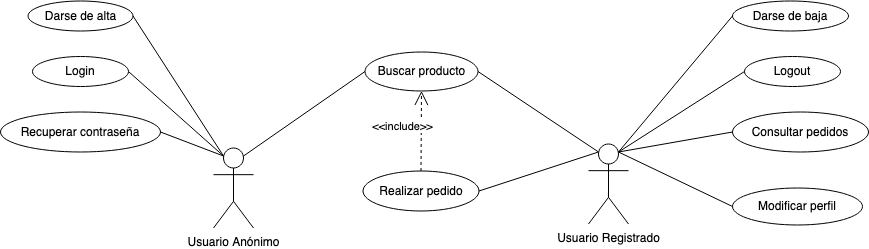
\includegraphics[width=\textwidth]{use-case_diagram}
                \caption{Diagrama de casos de uso}
                \label{fig:use-case_diagram}
            \end{figure}

            \paragraph{CU01\_Búsqueda}
            Proceso por el cual un usuario explora el catálogo y acaba por visualizar la página de un libro.
            \begin{itemize}
                \item[+] Actores implicados: Usuario Anónimo, Usuario Registrado.
                \item[+] Precondiciones: Usuario situado en cualquiera de las páginas que dan acceso al catálogo.
                \item[+] Flujo principal:
                \begin{enumerate}
                    \item[1.] El usuario hace click en alguna de las categorías principales mostradas a modo de catálogo flotante en la barra de navegación
                    o hace click en \emph{All Books}.
                    \item[2.] El sistema muestra la página de resultados de búsqueda.
                    \item[3.] El usuario hace click en alguno de los productos mostrados.
                    \item[4.] El sistema muestra la página del libro.
                \end{enumerate}
                \item[+] Flujo alternativo: \emph{refinamiento\_búsqueda}. El usuario altera en la página de resultados algún criterio de filtro.
                \begin{itemize}
                    \item[3.b.] El usuario selecciona/deselecciona algún criterio de filtro de entre los mostrados en la página de resultados de búsqueda.
                    \item[4.b.] El sistema vuelve al punto 2 del flujo principal.
                \end{itemize}
                \item[+] Flujo alternativo: \emph{búsqueda\_por\_texto}. El usuario introduce una cadena de texto en el cuadro de búsqueda.
                \begin{itemize}
                    \item[1.b.] El usuario introduce una cadena de texto en el cuadro de búsqueda y hace click en buscar.
                \end{itemize}
            \end{itemize}

            \paragraph{CU02\_Alta}
            Proceso por el cual se crea un nuevo usuario registrado.
            \begin{itemize}
                \item[+] Actores implicados: Usuario Anónimo.
                \item[+] Flujo principal:
                \begin{enumerate}
                    \item[1.] El usuario hace click en el link de nuevo registro, disponible en la página de \emph{login}.
                    \item[2.] El sistema presenta un formulario donde introducir la dirección de email y la contraseña.
                    \item[3.] El usuario introduce y envía la información pedida.
                    \item[4.] El sistema comprueba la información proporcionada.
                    \item[5.] El sistema crea una nueva cuenta de usuario, pero la mantiene inactiva a la espera de confirmar la dirección de email.
                    \item[6.] El sistema envía un email con un link de confirmación a la dirección proporcionada, e informa al usuario por pantalla.
                    \item[7.] El usuario accede a su email y hace click en el link enviado, confirmando que la dirección de email es suya.
                    \item[8.] El sistema activa la cuenta de usuario.
                    \item[9.] El sistema envía al usuario un email de bienvenida.
                    \item[10.] El sistema redirige al usuario a la página de \emph{login}.
                \end{enumerate}
                \item[+] Flujo alternativo: \emph{usuario\_ya\_registrado}. La dirección proporcionada se encuentra registrada en el sistema.
                \begin{itemize}
                    \item[5.b.] El sistema no crea una nueva cuenta de usuario. Por razones de seguridad, la manera en que el sistema informa al usuario tras esta situación es indistinguible del flujo principal, de forma que no se pueda deducir que ese email ya tiene cuenta asociada en el sistema.
                \end{itemize}
                \item[+] Flujo alternativo: \emph{link\_ya\_enviado}. El sistema está a la espera de la confirmación de un link válido en esta dirección de email.
                \begin{itemize}
                    \item[5.b.] El sistema no crea una nueva cuenta de usuario. Se informa al usuario acerca de una condición de error \-{}genérica, por seguridad\- en relación con la dirección de email proporcionada, pidiéndose que compruebe su dirección de email.
                \end{itemize}
                \item[+] Flujo excepcional: \emph{time\_out}. El usuario no confirma su dirección de email dentro de un plazo determinado.
                \begin{itemize}
                    \item[7.b.] El sistema detecta el timeout e invalida el link de confirmación enviado. Si el usuario hace click en el link caducado se le informa de dicha condición.
                \end{itemize}
            \end{itemize}

            \paragraph{CU03\_Login}
                Proceso por el cual un usuario se autentica en el sistema.
                \begin{itemize}
                    \item[+] Actores implicados: Usuario Anónimo.
                    \item[+] Flujo principal:
                    \begin{enumerate}
                        \item[1.] El usuario hace click en el link de \emph{login}, o intenta realizar alguna operación que requiera autenticación (por ejemplo, añadir un libro a la cesta).
                        \item[2.] El sistema presenta el formulario de acceso (dirección de email y la contraseña).
                        \item[3.] El usuario introduce y envía la información pedida.
                        \item[4.] El sistema comprueba las credenciales.
                        \item[5.] El sistema redirige al usuario a la página principal.
                    \end{enumerate}
                    \item[+] Flujo alternativo: \emph{fallo\_autenticación}. El email no se encuentra registrado en el sistema, o la contraseña proporcionada no es correcta.
                    \begin{itemize}
                        \item[5.b.] El sistema informa al usuario acerca de un fallo genérico de autenticación, de forma que, por razones de seguridad, no se pueda deducir si el email proporcionado se encuentra registrado en el sistema.
                    \end{itemize}
                    \item[+] Flujo alternativo: \emph{bloqueo\_cuenta}. El usuario anónimo realiza, dentro de un marco de tiempo (configurable), un número de intentos (configurable) de login con contraseña errónea.
                    \begin{itemize}
                        \item[5.b.] El sistema bloquea la cuenta asociada al email para prevenir ataques por fuerza bruta.
                        \item[6.] El sistema informa al usuario por pantalla y mediante el envío de un email.
                        \item[7.] Pasado el tiempo de seguridad (configurable), el sistema desbloquea la cuenta del usuario.
                    \end{itemize}
                    \item[+] Post-Condiciones: El usuario pasa a tener rol de usuario registrado en el sistema.
                \end{itemize}

            \paragraph{CU04\_RecuperarContraseña}
                Un usuario previamente registrado en el sistema intenta acceder al mismo, pero no recuerda su contraseña. El sistema intentará crear una nueva contraseña y enviarla al e-mail del usuario.
                \begin{itemize}
                    \item[+] Actores implicados: Usuario Anónimo.
                    \item[+] Flujo principal:
                    \begin{enumerate}
                        \item El usuario hace click en la opción \emph{¿olvidó su contraseña?}.
                        \item El sistema presenta un formulario donde introducir la dirección de email.
                        \item El usuario introduce y envía su dirección de email.
                        \item El sistema comprueba la dirección de email.
                        \item Comprobación correcta. El sistema envía un email con un link de confirmación a la dirección proporcionada, e informa de ello al usuario por pantalla.
                        \item Link no caducado. El usuario accede a su email y hace click en el link, confirmando que efectivamente la dirección proporcionada es la suya.
                        \item El sistema genera una nueva contraseña y se la asigna al usuario.
                        \item El sistema envía la nueva contraseña a la dirección de email del usuario, y le avisa de ello por pantalla.
                    \end{enumerate}
                    \item[+] Flujo alternativo: \emph{usuario\_no\_registrado}. La dirección proporcionada no se encuentra registrada en el sistema.
                    \begin{itemize}
                        \item[5.b.] El sistema no envía correo alguno pero, por razones de seguridad, desde el punto de vista del usuario este flujo alternativo es indistinguible del principal.
                    \end{itemize}
                    \item[+] Flujo excepcional: \emph{time\_out}. El usuario no confirma su dirección de email dentro de un plazo determinado.
                    \begin{itemize}
                        \item[6.b.] El sistema detecta el timeout e invalida el link de confirmación enviado. Si el usuario hace click en el link caducado se le informara de dicha condición.
                    \end{itemize}
                \end{itemize}

            \paragraph{CU05\_EditarPerfil}
                Proceso por el cual un usuario modifica alguno de los datos de su perfil personal.
                \begin{itemize}
                    \item[+] Actores implicados: Usuario Registrado.
                    \item[+] Flujo principal:
                    \begin{enumerate}
                        \item[1.] El usuario hace click en \emph{área personal}.
                        \item[2.] El sistema muestra la página de área personal, en donde se muestra el formulario de datos personales, rellenado con la información actual del usuario.
                        \item[3.] El usuario modifica los datos del formulario y lo envía al sistema.
                        \item[4.] El sistema comprueba los datos.
                        \item[5.] Comprobación correcta.El sistema actualiza la información del usuario.
                        \item[6.] El sistema muestra la página de inicio.
                    \end{enumerate}
                    \item[+] Flujo alternativo: \emph{error\_datos\_formulario}. Los datos proporcionados en el formulario de información personal no son válidos.
                    \begin{itemize}
                        \item[5.b.] El sistema regresa al punto 3 del flujo principal, e informa al usuario acerca del fallo producido.
                    \end{itemize}
                    \item[+] Flujo alternativo: \emph{cancelar}. El usuario cancela el proceso de edición de su información personal.
                    \begin{itemize}
                        \item[3.b.] El usuario hace click en el botón \emph{cancelar}. El sistema muestra la página de inicio.
                    \end{itemize}
                    \item[+] Post-Condiciones: El usuario ha alterado su información personal almacenada en la aplicación.
                \end{itemize}

            \paragraph{CU06\_RealizarPedido}
                Proceso por el cual un usuario realiza una compra a través de la aplicación web.
                \begin{itemize}
                    \item[+] Actores implicados: Usuario Registrado.
                    \item[+] Precondiciones: Desde cualquier página en la que se muestren libros (página de inicio, página de resultados de búsqueda o página de un libro) el usuario hace click en \emph{add to cart}, para uno o mas libros.
                    \item[+] Flujo principal:
                    \begin{enumerate}
                        \item[1.] El usuario hace click en el icono de la cesta.
                        \item[2.] El sistema muestra la página de la cesta del usuario, con todos los libros contenidos en el mismo.
                        \item[3.] El usuario puede aumentar o disminuir el número de unidades de un libro, o incluso eliminarlo por completo, y hace click en \emph{checkout}.
                        \item[4.] El sistema comprueba la disponibilidad de los libros contenidos en la cesta.
                        \item[5.] Stock suficiente. El sistema muestra la página de checkout, con el formulario de datos de envío y pago, y el resumen de la compra.
                        \item[6.] El usuario completa los datos de envío y de pago y hace click en \emph{Pay}.
                        \item[7.] El sistema tramita el pago.
                        \item[8.] Pago ok. El sistema registra el nuevo pedido.
                        \item[9.] El sistema confirma al usuario por pantalla y por email que el pedido se ha realizado con éxito.
                    \end{enumerate}
                    \item[+] Flujo alternativo: \emph{stock\_insuficiente}. No hay stock suficiente para satisfacer el contenido de la cesta.
                    \begin{itemize}
                        \item[5.b.] El sistema vuelve al punto 2 del flujo principal, informando al usuario de los libros para los cuales no hay stock suficiente.
                        \item[3.b.] El usuario reduce la cantidad demandada de los libros correspondientes y hace click en \emph{checkout}.
                    \end{itemize}
                    \item[+] Flujo alternativo: \emph{error\_pago}. Error al efectuar el pago.
                    \begin{itemize}
                        \item[8.b.] El sistema vuelve al punto 5 del flujo principal, informando al usuario del problema respecto al pago.
                    \end{itemize}
                    \item[+] Flujo excepcional: \emph{libro\_eliminado}. Algún libro de la cesta ya no esta disponible en el sistema.
                    \begin{itemize}
                        \item[5.b.] El sistema elimina de la cesta automáticamente los libros que el administrador haya deshabilitado.
                        \item[6.b.] El sistema vuelve al punto 2 del flujo principal, informando al usuario de los libros que han sido eliminados.
                    \end{itemize}
                    \item[+] Post-Condiciones: El usuario ha efectuado un nuevo pedido.
                \end{itemize}

            \paragraph{CU07\_ConsultarPedido}
                Proceso por el cual un usuario consulta el historial de pedidos que ha realizado.
                \begin{itemize}
                    \item[+] Actores implicados: Usuario Registrado.
                    \item[+] Flujo principal:
                    \begin{enumerate}
                        \item[1.] El usuario hace click en \emph{My Purchases} en la barra de navegación.
                        \item[2.] El sistema muestra la página de los pedidos del usuario.
                        \item[3.] El usuario puede expandir-contraer la información mostrada relativa a un pedido.
                    \end{enumerate}
                \end{itemize}

            \paragraph{CU08\_Baja}
                Proceso por el cual un usuario elimina su cuenta de la tienda online.
                \begin{itemize}
                    \item[+] Actores implicados: Usuario Registrado.
                    \item[+] Flujo principal:
                    \begin{enumerate}
                        \item[1.] El usuario hace click en \emph{área personal}.
                        \item[2.] El sistema muestra la página de área personal.
                        \item[3.] El usuario selecciona \emph{eliminar cuenta}.
                        \item[4.] El sistema muestra el formulario de eliminación de cuenta.
                        \item[5.] El usuario completa y envía el formulario.
                        \item[6.] El sistema comprueba los datos.
                        \item[7.] Comprobación correcta. El sistema actualiza el estado del usuario y envía un email de confirmación.
                        \item[8.] El sistema muestra la página de inicio.
                    \end{enumerate}
                    \item[+] Flujo alternativo: \emph{error\_datos\_formulario}. La contraseña proporcionada en el formulario de baja no es correcta.
                    \begin{itemize}
                        \item[7.b.] El sistema regresa al punto 4 del flujo principal, e informa al usuario acerca del fallo producido.
                    \end{itemize}
                    \item[+] Flujo alternativo: \emph{cancelar}. El usuario cancela el proceso de baja.
                    \begin{itemize}
                        \item[5.b.] El usuario cancela el proceso de baja. El sistema regresa al punto 2 del flujo principal.
                    \end{itemize}
                    \item[+] Post-Condiciones: El usuario ya no figura como dado de alta en la aplicación.
                \end{itemize}

            \paragraph{CU09\_Logout}
                Proceso por el cual un usuario cierra su sesión en el sistema.
                \begin{itemize}
                    \item[+] Actores implicados: Usuario Registrado.
                    \item[+] Precondiciones: el usuario está con su sesión abierta en el sistema.
                    \item[+] Flujo principal:
                    \begin{enumerate}
                        \item[1.] El usuario hace click en el link de \emph{logout}.
                        \item[2.] El sistema cierra la sesión del usuario.
                        \item[3.] El sistema muestra la página de inicio.
                    \end{enumerate}
                    \item[+] Post-Condiciones: El usuario ha efectuado el logout con éxito.
                \end{itemize}


    \section{Diseño}
    En este apartado se ofrece una descripción de las decisiones tomadas a nivel de diseño de la aplicación web.
    \subsection{Arquitectura del Sistema}
    Desde un punto de vista lo suficientemente alejado como para no percibir los detalles internos, la aplicación web está organizada siguiendo la arquitectura clásica cliente-servidor-datos. Hoy en día, quizás, esta no sea la organización más vanguardista. Los términos \emph{serverless}, \emph{microservicios} o \emph{single-page-application} son los que con mayor eco resuenan en la industria web actual.
    
    \begin{figure}[h]
    	\centering
    	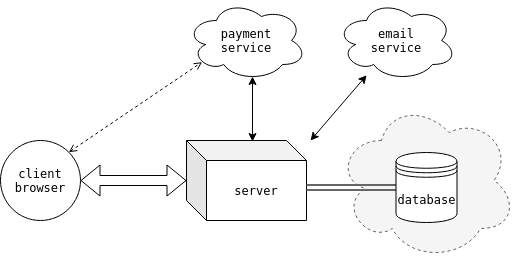
\includegraphics[width=\textwidth]{desing_general}
    	\caption{Modelo del sistema}
    	\label{fig:desing_general}
    \end{figure}
    
    Como muchas tendencias dentro del mundo de la computación, estos términos no están del todo delimitados, ofreciendo en ocasiones diferentes interpretaciones y/o solapamientos entre sí. Serverless hace mención a aquellas aplicaciones web que en su mayor parte, o por completo, incorporan servicios cloud de terceras partes para gestionar su propia lógica de negocio. La arquitectura de microservicios está muy relacionada con lo anterior, ya que esta concibe las aplicaciones como un agregado de servicios muy especializados ejecutados de forma independiente, puede que en máquinas remotas, que se comunican entre sí de manera ligera y eficiente. Por su parte, las SPA usan la elevada capacidad de cómputo de los clientes actuales para trasladar allí parte de la lógica que tradicionalmente implementa el servidor. En una SPA o bien todo el contenido HTML, JavaScript y CSS es cargado una sola vez, o bien se carga dinámicamente bajo demanda, normalmente como respuesta a las acciones del usuario, dando así una mayor sensación de fluidez.
    
    No obstante, a pesar de las muchas ventajas que presentan estas formas de enfocar las aplicaciones web, se ha optado por la arquitectura clásica (con pinceladas, como se verá, de aspectos serverless y SPA), y el motivo es doble:
    
    \begin{itemize}
    	\item[-] Antes del 2 va el 1. El punto de partida en el desarrollo de la presente aplicación web fue el de prácticamente nulos conocimientos sobre esta rama de la informática. En este escenario, antes de estudiar directamente las arquitecturas surgidas en los últimos años, se ha preferido estudiar la arquitectura clásica, en el convencimiento de que es el camino formativo correcto.
    	\item[-] Tecnología viva. En contra de lo que hace unos años algunas voces avanzaban, la arquitectura browser-server-database no está muerta y previsiblemente no lo va a estar. Esta es una tecnología madura, robusta y muy extendida. Aunque es muy cierto que su cuota de mercado ha descendido en pro de otras arquitecturas más recientes, muestra tener un suelo estable y un lugar propio dentro de las tecnologías web. En parte esto es así porque, como casi siempre, no es oro todo lo que reluce. Las arquitecturas modernas no son la perfección, mostrando tener algunos puntos débiles [bib ref].
    \end{itemize}
    
    En la figura \ref{fig:desing_general} se presenta un esquema de la arquitectura de la aplicación web. Como se aprecia, responde a la mencionada arquitectura clásica cliente-servidor-datos. No obstante, existen ciertos elementos que descansan en servicios cloud externos, dotando a la aplicación de cierto carácter serverless. Así, el servicio de pagos es ofrecido por Stripe (ver \ref{sec:stripe}). Como se aprecia en la figura \ref{fig:desing_general}, existe una vía de comunicación directa entre el cliente y Stripe. Esto es así para garantizar que la aplicación web no tiene nunca acceso a los datos confidenciales de pago del cliente (p.e., número de la tarjeta de crédito), sino que esta información es enviada directamente desde el cliente a Stripe. Por su parte, el servicio de correo es delegado en Gmail, a través de la capa de abstracción que Spring Framework ofrece de la API JavaMail. Y, por último, la base de datos. Este caso es especial porque dependiendo del entorno de ejecución se puede asimilar a un servicio cloud o no. En este sentido, cuando el entorno de ejecución es producción, la base datos es accedida como un servicio que AWS presta a Heroku.
        
    Por otro lado, centrando ahora la atención en la organización interior de la aplicación, el principio de diseño protagonista ha sido la \textbf{separación de responsabilidades} (\emph{separation of concerns}, SoC). Este principio es un viejo conocido en el mundo de la ingeniería, haciendo manejables problemas que de otra manera serían muy costosos, si no directamente intratables.
    
    
    \subsubsection[Inversión de Control]{Inversión de Control - Inyección de Dependencias} \label{sec:ioc}
    Un primer paso en la división de responsabilidades es la separación de la construcción y el uso. Piénsese por ejemplo en un aeropuerto. Los trabajos que se deben llevar a cabo, las herramientas necesarias, el personal técnico implicado, etc. son distintos en la fase de construcción que durante su posterior explotación. En este sentido, los sistemas software no son excepción. Las tareas a realizar cuando la aplicación arranca son diferentes de las que se llevan a cabo durante el normal funcionamiento posterior. Por tanto, la lógica de arranque, encargada de crear los objetos y de resolver y conectar sus dependencias, debe ser separada de la lógica que comienza tras el arranque.
    
    Un mecanismo efectivo para separar la construcción del uso es la \textbf{inyección de dependencias} (\emph{dependency injection}, DI), que, tal como explica Martin Fowler en su \href{https://martinfowler.com/articles/injection.html}{artículo seminal} en la materia [bib ref], es un tipo de \textbf{inversión de control} (\emph{inversion of control}, IoC) para la gestión de dependencias. Por inversión de control se entiende la técnica de traspasar las responsabilidades secundarias de un objeto a otros objetos especializados para el propósito. Así, en el contexto de gestión de dependencias, un objeto no debe asumir la responsabilidad de instanciar él mismo sus dependencias. En su lugar, debe ceder esta responsabilidad a otra entidad especializada, invirtiendo así el control. Debido a que la configuración inicial es una cuestión global, esta entidad especializada será la rutina \emph{main} o un contenedor especializado en este propósito. En el caso de la presente aplicación web se ha usado el contenedor de inyección de dependencias del mundo Java líder en la actualidad, Spring Framework (ver \ref{sec:spring}). Como se muestra en el listado \ref{list:ioc}, el contenedor es invocado en la primera y única instrucción de \emph{main}.
    \\
    
    \begin{lstlisting}[language=Java,caption=Inversión de control de dependencias,label=list:ioc]
    @SpringBootApplication
    public class FirstmarketApplication {
    
    	public static void main(String[] args) {
    		//el contenedor de IoC se encarga de crear los objetos y 
    		//de resolver sus interdependencias
    		SpringApplication.run(FirstmarketApplication.class, args);
    	}
    
    }
    \end{lstlisting}
    
    A modo de ejemplo, las figuras \ref{fig:di_bookRepository}, \ref{fig:di_bookServer} y \ref{fig:di_bookController} muestran, respectivamente, los diagramas de inyección de dependencias para las tres capas de abstracción relacionadas con los libros: \emph{bookRepository}, \emph{bookServer} y \emph{bookController}. La flecha verde, que parte siempre de \emph{firstmarketApplication}, indica que el objeto apuntado ha sido creado por el contenedor de IoC. Las flechas azules significan que el objeto apuntado (la dependencia) ha sido insertado por el contenedor de IoC en el objeto apuntador.

	\begin{figure}[htb!]
		\centering
		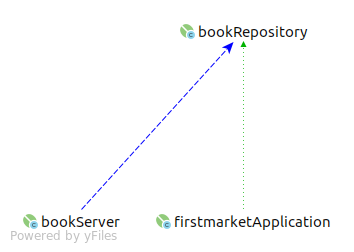
\includegraphics[width=0.6\textwidth]{di_bookRepository}
		\caption{Creación e inyección de dependencias en BookRepository}
		\label{fig:di_bookRepository}
	\end{figure}

	\begin{figure}[htb!]
		\centering
		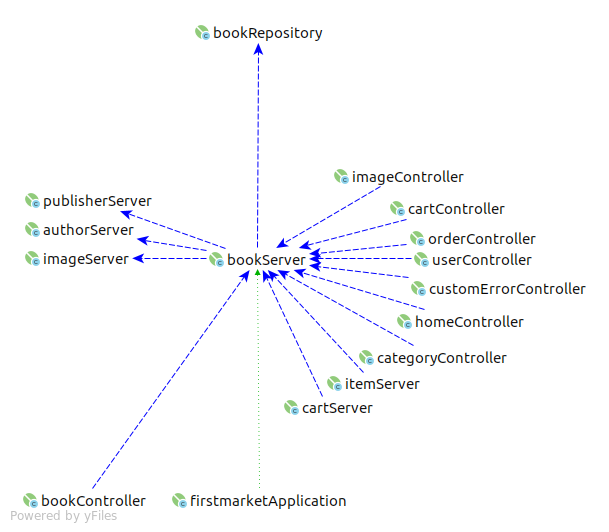
\includegraphics[width=\textwidth]{di_bookServer}
		\caption{Creación e inyección de dependencias en BookServer}
		\label{fig:di_bookServer}
	\end{figure}

	\begin{figure}[htb!]
		\centering
		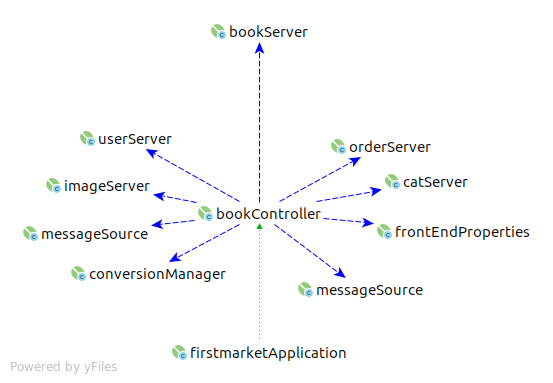
\includegraphics[width=\textwidth]{di_bookController}
		\caption{Creación e inyección de dependencias en BookContoller}
		\label{fig:di_bookController}
	\end{figure}
    
    \subsubsection{Capas funcionales} \label{sec:design_layer}
    Otro paso importante dado en la dirección de separar las responsabilidades es la división funcional del código en tres capas: web, negocio y persistencia. Estas capas están contenidas dentro del paquete \emph{core}, y están inspiradas en el patrón de diseño \emph{Fron Controller}, que es el que ordena, a su vez, la infraestructura web que proporciona Spring Framework (ver sección \ref{sec:spring}).
    
    \begin{figure}[htb!]
    	\centering
    	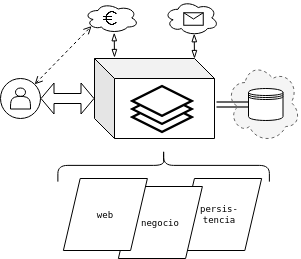
\includegraphics[width=0.75\textwidth,keepaspectratio]{desing_layer}
    	\caption{Modelo del sistema en capas funcionales}
    	\label{fig:desing_layer}
    \end{figure}
    
    La capa web se encarga de gestionar las peticiones HTTP encauzadas a través del \emph{DispatcherServler} y de resolver y generar el contenido HTML. A parte de toda la infraestructura que ofrece Spring Framework para esta tarea, se ha desarrollado una serie de \emph{controladores} (anotados con \emph{@Controller}), contenidos en el paquete \emph{core.controller} (ver figura \ref{fig:package_controller}), que sirven un conjunto de \emph{vistas}, contenidas en \emph{classpath: resources/templates}. Esta capa recibe el servicio de la capa de negocio.
    	
   	\begin{figure}[htb!]
   		\centering
   		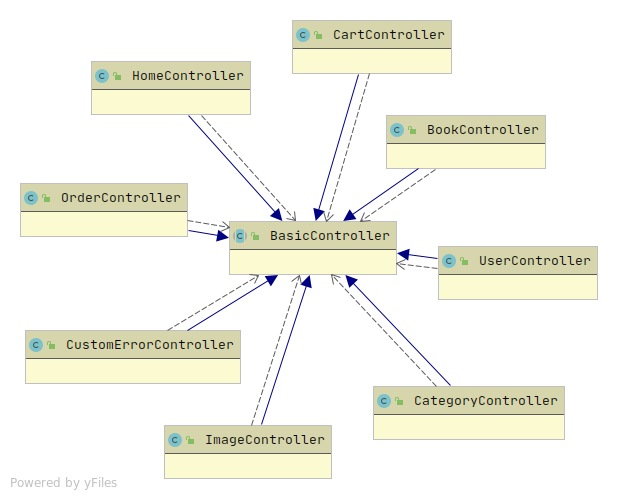
\includegraphics[width=0.7\textwidth,keepaspectratio]{package_controller}
   		\caption{Diagrama del paquete core.controller}
   		\label{fig:package_controller}
   	\end{figure}

   	\begin{figure}[htb!]
   		\centering
   		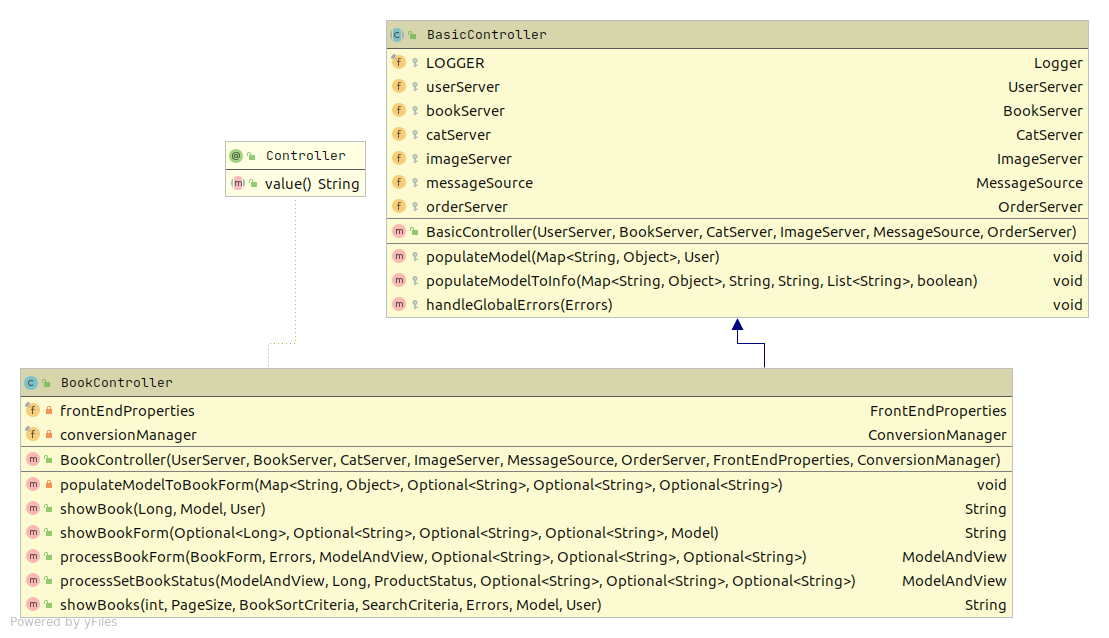
\includegraphics[width=\textwidth,keepaspectratio]{detail_bookController}
   		\caption{Detalle de la clase BookController}
   		\label{fig:detail_bookController}
   	\end{figure}
    	
   	En la capa de negocio reside la lógica (objetos anotados con \emph{@Service}) que modela el funcionamiento de una tienda de libros a través del código contenido en el paquete \emph{core.service} (ver figura \ref{fig:package_service}). Esta capa da servicio a la capa web y a sí misma, mientras que se apoya en el servicio que le ofrece la capa de persistencia.
    	
   	\begin{figure}[htb!]
		\centering
		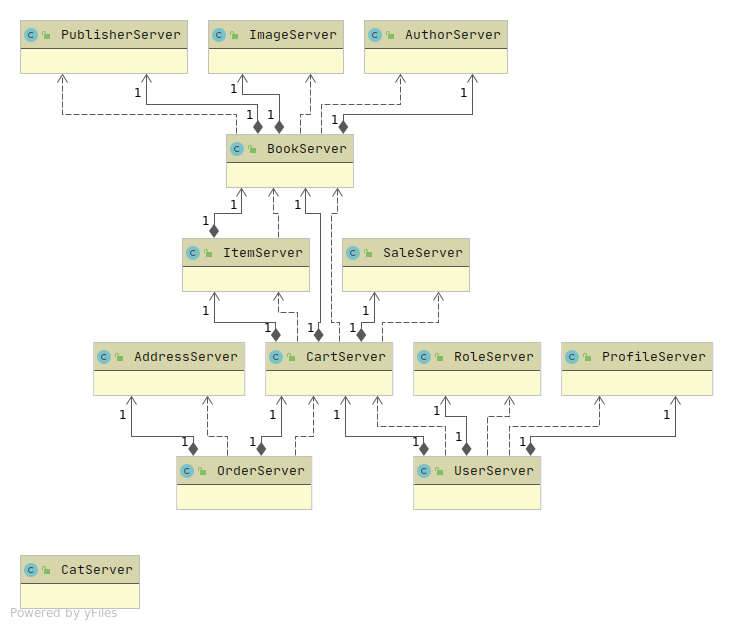
\includegraphics[width=\textwidth,keepaspectratio]{package_service}
		\caption{Diagrama del paquete core.service}
		\label{fig:package_service}
	\end{figure}

	\begin{figure}[htb!]
		\centering
		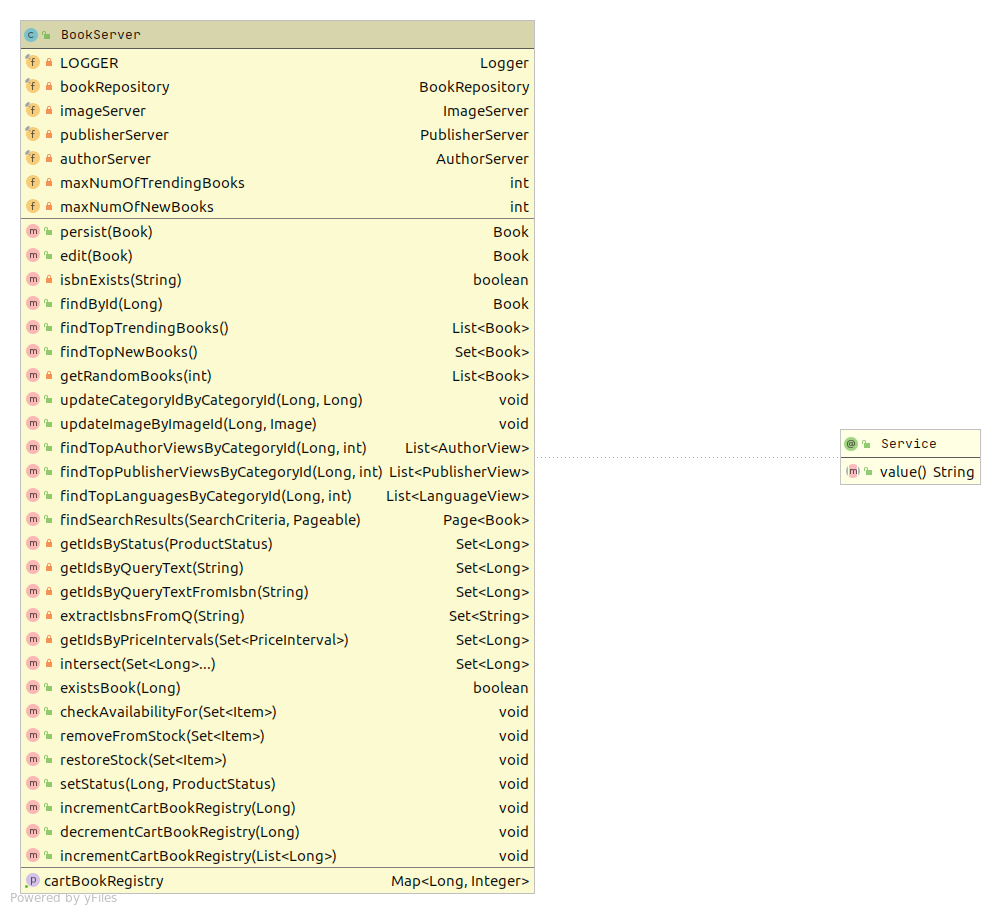
\includegraphics[width=\textwidth,keepaspectratio]{detail_bookServer}
		\caption{Detalle de la clase BookServer}
		\label{fig:detail_bookServer}
	\end{figure}

   	La capa de persistencia sigue el patrón de diseño \href{https://thorben-janssen.com/implementing-the-repository-pattern-with-jpa-and-hibernate/}{\emph{Repositorio}}. Así, toma el control de todos los aspectos relacionados con la solución concreta de almacenamiento y manipulación de los datos, desacoplando por completo esta funcionalidad de la lógica de negocio, a la cual sirve mediante un conjunto de interfaces (anotadas con \emph{@Repository}) definidas en \emph{core.data} (ver figura \ref{fig:package_data}).
    	
   	\begin{figure}[htb!]
   		\centering
   		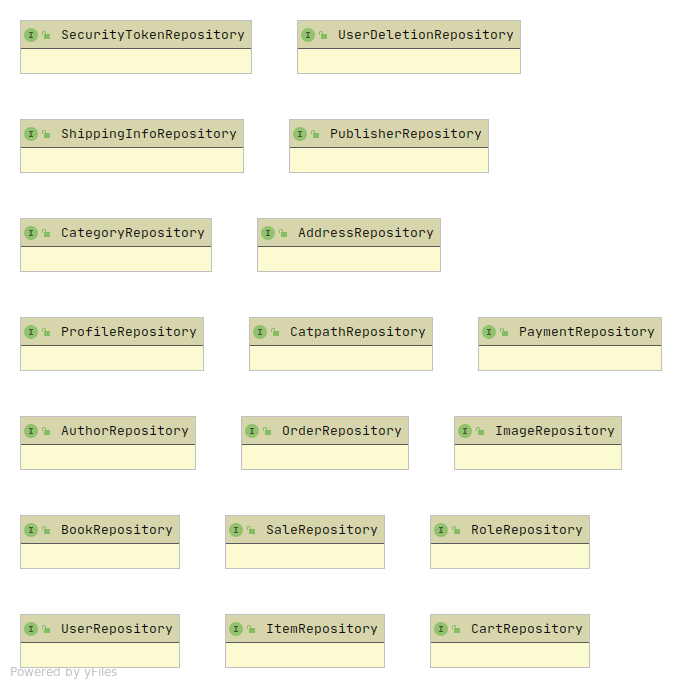
\includegraphics[width=\textwidth,keepaspectratio]{package_data}
   		\caption{Diagrama del paquete core.data}
   		\label{fig:package_data}
   	\end{figure}
   	
   	\begin{figure}[htb!]
   		\centering
   		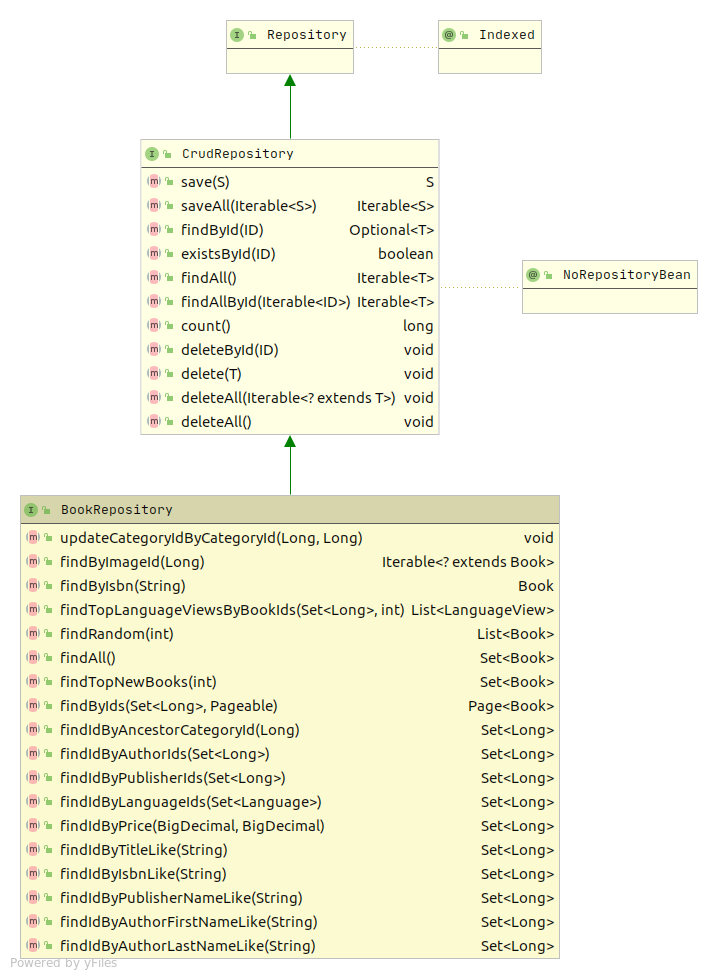
\includegraphics[width=\textwidth,keepaspectratio]{detail_bookRepository}
   		\caption{Detalle de la interfaz BookRepository}
   		\label{fig:detail_bookRepository}
   	\end{figure}
    	
    
    \subsection{Modelo de Datos}
    Para dar solución al problema presentado (la venta de libros online) se ha realizado un modelado de entidades del mundo real. Estas entidades se encuentran definidas en el paquete \emph{core.model}. En la figura \ref{fig:package_model} se muestra el diagrama de clases de este paquete. Este modelo encuentra una traducción directa en las entidades gestionadas en la base datos. En las figuras \ref{fig:er_simple_diagram} y \ref{fig:er_expanded_diagram} se ofrecen, respectivamente, los diagramas entidad relación sin y con las propiedades de los objetos visibles.
    
    \begin{figure}[htb!]
    	\centering
    	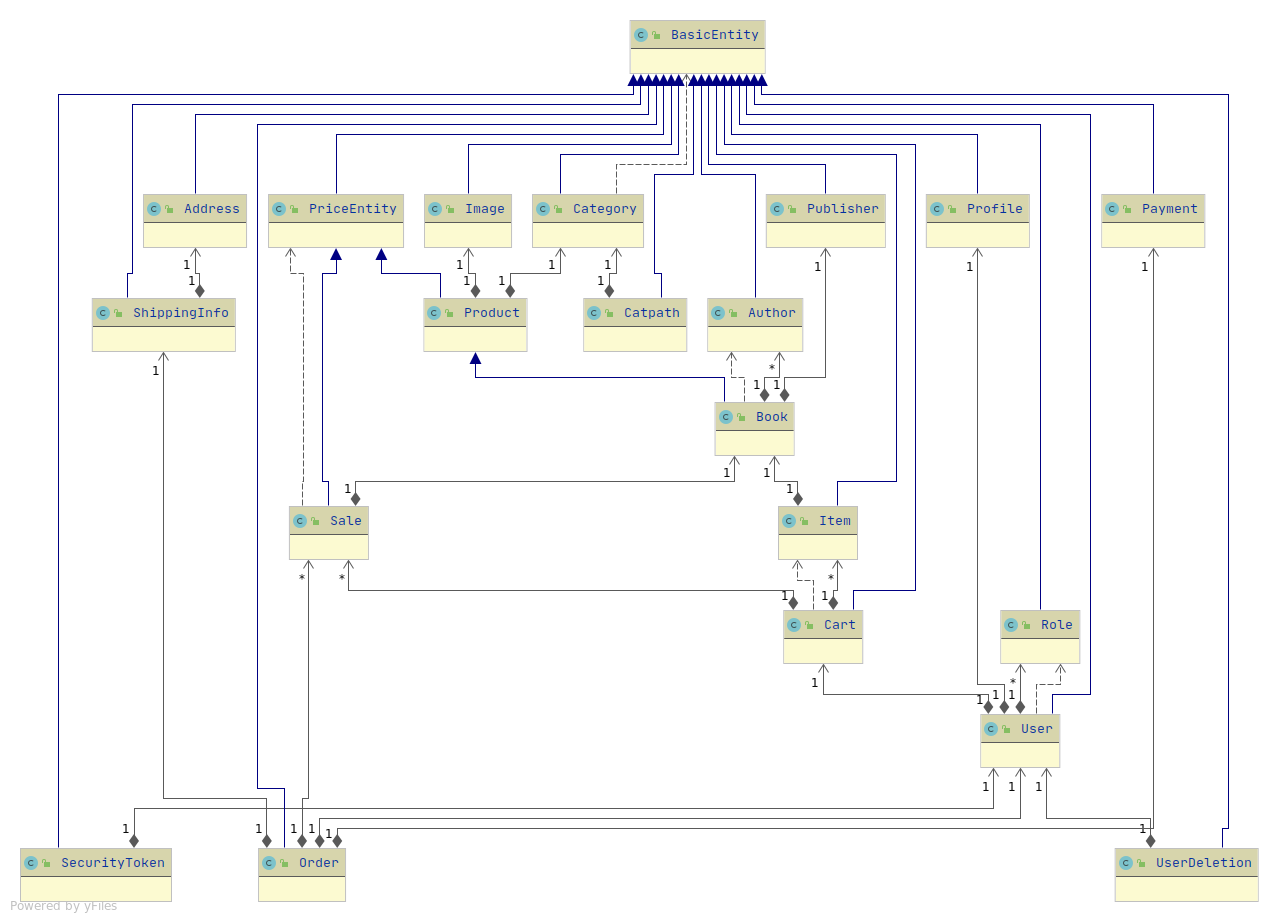
\includegraphics[height=\textwidth,angle=90,origin=c]{package_model}
    	\caption{Diagrama de clases del paquete core.model}
    	\label{fig:package_model}
    \end{figure}

	\begin{figure}[htb!]
		\centering
		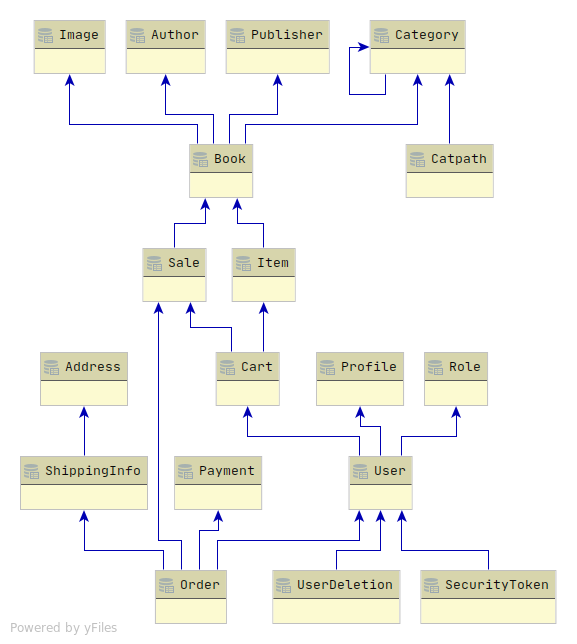
\includegraphics[width=\textwidth,keepaspectratio]{er_simple_diagram}
		\caption{Diagrama entidad-relación}
		\label{fig:er_simple_diagram}
	\end{figure}

	\begin{figure}[htb!]
		\centering
		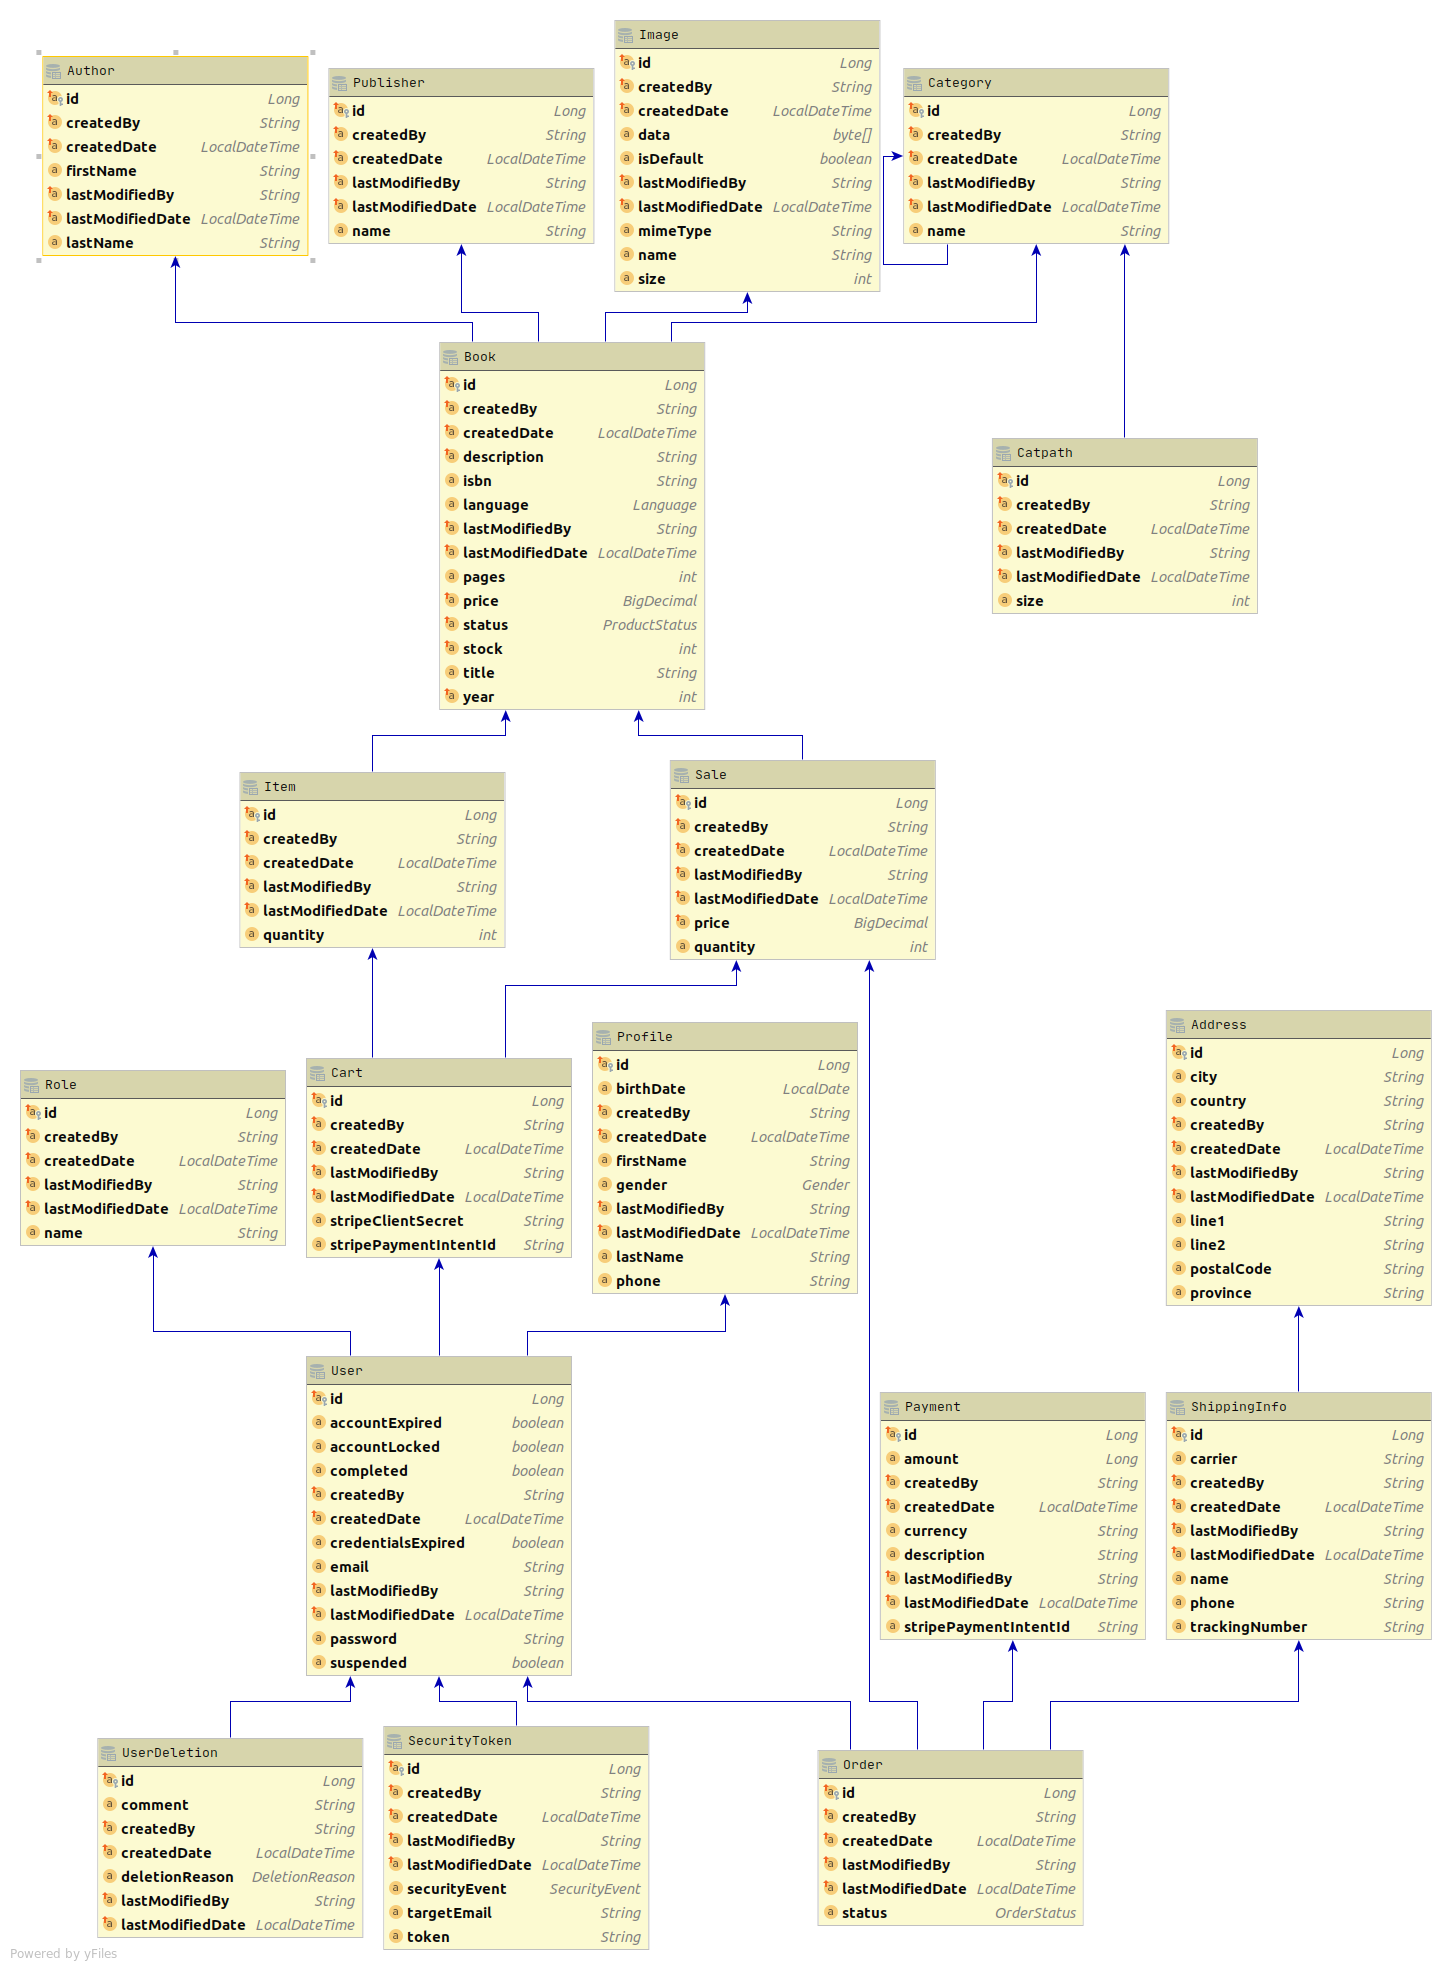
\includegraphics[width=\textwidth,keepaspectratio]{er_expanded_diagram}
		\caption{Diagrama entidad-relación expandido}
		\label{fig:er_expanded_diagram}
	\end{figure}

    \section{Implementación}
    La materialización del análisis y diseño detallado en las secciones anteriores lo conforma el conjunto software que se incluye en el CD distribuido con la presente memoria. No obstante, en este apartado se ha querido comentar ciertos aspectos relevantes, que por la dificultad presentada y/o por el papel clave dentro de la aplicación merecen mención especial.
    
    \subsection{Stack Tecnológico}
    En este apartado se ofrece un comentario sobre las principales decisiones tomadas acerca de las tecnologías empleadas en el desarrollo de la aplicación web.
    
    \subsubsection{Git}
    Como se comentó en la exposición de motivos, Git es una tecnología clave para el control de versiones, y desde el principio se puso el foco en ella. Aunque existen otras herramientas muy válidas, como Mercurial, la decisión fue seguir la tendencia global.
    
    Formalmente, Git es un sistema de control de versiones distribuido, permitiendo gestionar los cambios introducidos en un conjunto de ficheros, conocido como \emph{repositorio}, por un número arbitrario de personas. Sus principales características son:
    
    \begin{itemize}
    	\item[-] \textbf{Basado en instantáneas}. Otros sistemas de control de versiones tratan la información que almacenan como un conjunto de archivos más sus cambios a lo largo del tiempo, los incrementos. En cambio, Git piensa en sus datos más como una serie de instantáneas de un sistema de archivos en miniatura. Así, cada vez que se efectúa un \emph{commit} o se guarda el estado de un proyecto, Git toma una fotografía de cómo se están todos los archivos en ese momento y almacena una referencia a esa instantánea. Además, para ser eficiente, si los archivos no han cambiado no almacena el archivo nuevamente, sino un enlace al archivo idéntico anterior almacenado. En resumen, Git trata los datos que gestiona como una secuencia de capturas.
    	\item[-] \textbf{Trabajo en local}. Git es un sistema distribuido que permite que todos los implicados en un proyecto tengan en su máquina una copia completamente funcional del repositorio. Así, la mayoría de las operaciones necesitan sólo archivos y recursos locales para funcionar, siendo muy poco lo que no se puede hacer sin conexión a Internet. 
    	\item[-] \textbf{Integridad de la información}. Es casi imposible que algo varíe en los archivos gestionados por Git sin que el sistema lo detecte, dado que a todos estos archivos se les aplica la función \emph{hash} SHA-1, obteniendo como resultado una cadena de 40 caracteres hexadecimales. Esta cadena es luego usada en todo momento para referenciar el contenido usado para generarla.
    	\item[-] \textbf{Seguridad ante accidentes}. Con Git es muy difícil que, una vez realizado un \emph{commit}, se pierda el trabajo almacenado.
    \end{itemize}
    
    En el presente proyecto el uso de Git ha sido intensivo y fundamental. El repositorio del proyecto, alojado en GitHub, puede ser accedido \href{https://github.com/misrraimsp/firstmarket}{aquí}.
    
    \subsubsection{Java}
    Una de las primeras decisiones que se tuvo que tomar fue qué lenguaje de programación emplear para construir la aplicación web, ya que aunque en la especificación de la oferta del proyecto se establecía que este debiera ser PHP, a posteriori la libertad fue total. Esta no es una decisión trivial, ya que determina en gran medida el resto del stack tecnológico utilizado. Tras una exploración de las diferentes alternativas, y dado el background adquirido a lo largo del plan de estudios, la opción tomada fue Java. Es cierto que existen alternativas potentes en el mundo de la programación web, pero también lo es que Java ocupa una posición muy madura y asentada en la industria, con un entorno de recursos disponibles para el estudiante defícilmente superable, y con una perspectiva de futuro, como mínimo, estable. La decisión tomada primó profundidad antes que anchura, en el sentido de preferir aumentar y depurar las habilidades en Java antes de expandir a otros lenguajes. Por supuesto, esto es muy discutible, pero se creyó que era la opción correcta.
    
    Resaltar, además, que la versión utilizada ha sido Java 11, que en la actualidad es la más reciente que ofrece soporte a largo plazo (LTS, \emph{Long Term Support}).
    \\
    
    Java es un lenguaje que, como muchos otros, ha ido evolucionando con el tiempo, dando como resultado un conjunto de capacidades muy variado. En 2014, con la publicación de Java 8, el lenguaje experimentó una de las mayores expansiones, si no la mayor, de su historia. En ese momento se le introdujeron potentes capacidades de programación declarativa, como las \emph{Labmda Expressions} y la \emph{Stream API}, que, en cierto modo, han revolucionado la programación Java (véase, por ejemplo, el framework de desarrollo de aplicaciones web \href{http://sparkjava.com/}{Spark}, que sólo usa capacidades Java 8+)
    \\
    
    \begin{lstlisting}[language=Java,caption=Programación declarativa con Java,label=list:java_declarative]
    private Set<Long> getIdsByExcludedStatus(ProductStatus excludedStatus) {
    return bookRepository
    .findAll()
    .stream()
    .filter(book -> !book.getStatus().equals(excludedStatus))
    .map(Book::getId)
    .collect(Collectors.toSet())
    ;
    }
    \end{lstlisting}
    
    Como se ha comentado, una de las intenciones de usar la tecnología Java era precisamente profundizar en su conocimiento. Así, se ha aprovechado el desarrollo de la presente aplicación para estudiar estas capacidades declarativas, aplicándolas progresivamente. Como ejemplo, en el listado \ref{list:java_declarative} se muestra la implementación del método \emph{getIdsByExcludedStatus}, perteneciente a la clase \emph{BookServer}. Se puede apreciar la facilidad de lectura que el estilo declarativo proporciona, además de la potencia expresiva. 
    \\
    
    También es necesario comentar un par de librerías que merecen especial mención, por la relevancia que han tenido en el proyecto:
    
    \paragraph{Project Lombok}
    Aparte del nombre de una isla indonesia (como Java), Lombok es una librería Java destinada a aumentar la productividad. Se encarga de suprimir la necesidad de especificar cierto código repetitivo, como los constructores, los \emph{getters} y los \emph{setters}, o los \emph{equals} y los \emph{hashCode}. Así, como se muestra en el listado \ref{list:lombok_close}, a través de anotaciones se puede ahorrar una grandísima cantidad de código, que es generado por esta herramienta automáticamente antes de la compilación.
    \\
    
    \begin{lstlisting}[language=Java,caption=Clase \emph{Role} usando las anotaciones Lombok,label=list:lombok_close]
    package misrraimsp.uned.pfg.firstmarket.core.model;
    
    import lombok.Data;
    import lombok.EqualsAndHashCode;
    
    import javax.persistence.Entity;
    
    @Data
    @EqualsAndHashCode(callSuper = true)
    @Entity
    public class Role extends BasicEntity {
    
    	private String name;
    
    }
    \end{lstlisting}
    
    No obstante, en cualquier momento se puede efectuar un \emph{Delombok} y ver el código generado, como se muestra en el listado \ref{list:lombok_open}. Como se aprecia, la cantidad de código ahorrado es más que significativa.
    \\
    
    \begin{lstlisting}[language=Java,caption=Clase \emph{Role} tras efectuar un \emph{Delombok},label=list:lombok_open]
    package misrraimsp.uned.pfg.firstmarket.core.model;
    
    import javax.persistence.Entity;
    
    @Entity
    public class Role extends BasicEntity {
    
	    private String name;
	    
	    public Role() {
	    }
	    
	    public String getName() {
	    	return this.name;
	    }
	    
	    public void setName(String name) {
	    	this.name = name;
	    }
	    
	    public String toString() {
	    	return "Role(name=" + this.getName() + ")";
	    }
	    
	    public boolean equals(final Object o) {
		    if (o == this) return true;
		    if (!(o instanceof Role)) return false;
		    final Role other = (Role) o;
		    if (!other.canEqual((Object) this)) return false;
		    if (!super.equals(o)) return false;
		    final Object this$name = this.getName();
		    final Object other$name = other.getName();
		    if (this$name == null ? other$name != null : !this$name.equals(other$name)) return false;
		    return true;
	    }
	    
	    protected boolean canEqual(final Object other) {
	    	return other instanceof Role;
	    }
	    
	    public int hashCode() {
		    final int PRIME = 59;
		    int result = super.hashCode();
		    final Object $name = this.getName();
		    result = result * PRIME + ($name == null ? 43 : $name.hashCode());
		    return result;
	    }
    }
    \end{lstlisting}
    
    \paragraph{SLF4J - Logback}
    SLF4J (Simple Logging Facade for Java) es una API Java para tareas de registro que implementa el patrón de diseño \href{https://en.wikipedia.org/wiki/Facade_pattern}{\emph{facade}}, el cual permite desacoplar completamente el código de la aplicación de la tecnología específica de registro que subyaga bajo la fachada.
    
    Logback es la tecnología elegida que en el presente proyecto se conecta como backend de SLF4J. Se trata de una librería moderna, diseñada por el fundador de la famosa Log4j (Ceki Gülcü), y que pretende ser su sucesora.
    
    La configuración se encuentra en el fichero \emph{classpath: logback-spring.xml}, donde se detallan todos los aspectos relevantes, como el formato utilizado en los registros o la política de escritura y rotación de los ficheros de registro producidos.
    
    Esta es una de las funcionalidades añadidas al proyecto que, aún siendo muy humilde, ha tenido enorme impacto en la facilidad de desarrollo y mantenimiento. Es clave que desde fases tempranas se tenga un sistema de registro, el cual poder utilizar, por ejemplo, en las múltiples tareas de depuración que se deben llevar a cabo casi constantemente.
    \\
    
    Por último, un apunte acerca del entorno de desarrollo utilizado. Durante las primeras semanas se usó el mismo que en toda la carrera: Eclipse. Sin embargo, en el transcurso de una formación en Spring tomada en fases iniciales del proyecto, se entró en contacto con \textbf{IntelliJ IDEA}. Desde entonces ese fue el IDE empleado, destacándose su capacidad de aumentar la productividad y su facilidad de uso.
    
    \subsubsection{Apache Maven}
    En el mundo del desarrollo software una fase de especial importancia es aquella encargada de transformar todos los archivos de código fuente del proyecto en un paquete susceptible de ser distribuido, instalado y ejecutado en cualquier máquina. A esto se le conoce como el proceso de construcción del proyecto, y representa una tarea no trivial desde el momento en que el proyecto en sí adquiere cierta complejidad.
    
    Antiguamente, este proceso tenía que ser diseñado e implementado \emph{ad hoc}, de una manera específica para cada proyecto. Sin embargo, en la actualidad este proceso se encuentra altamente optimizado. En el caso del mundo Java las principales herramientas empleadas al efecto son Apache Maven y Gradle.
    
    En el presente proyecto se ha optado por utilizar Apache Maven. La justificación reside en que el punto de partida fue el total desconocimiento de este tipo de tecnologías, y al representar Gradle, aparentemente, una suerte de superconjunto o mejora sobre Apache Maven, se juzgó conveniente tomar a este último como puerta de entrada o primer escalón, teniendo en cuenta, además, que Apache Maven aún posee una profunda implantación en la industria y la documentación y recursos de todo tipo para su estudio es ingente.
    
    Apache Maven supuso una revolución en la forma de construir software en el mundo Java. Pero esta herramienta va más allá, siendo concebida como una utilidad de gestión y de comprensión de los proyectos software. Tal como se explica en su \href{https://maven.apache.org/what-is-maven.html}{web oficial}, sus principales objetivos son:
    
    \begin{itemize}
    	\item[-] Facilitar la construcción software.
    	\item[-] Homogeneizar el proceso de construcción software.
    	\item[-] Ofrecer un lenguaje común a la hora de obtener información sobre un proyecto, es decir, establecer una manera homogénea de \emph{definir} a un proyecto software.
    	\item[-] Incentivar buenas prácticas de desarrollo software.
    \end{itemize}
    
    Las características que han permitido a Apache Maven alcanzar estos objetivos descansan en gran medida en:
    
    \begin{itemize}
    	\item[-] \textbf{Convención sobre configuración}. Como también se comentará en la sección \ref{sec:spring}, este principio de diseño persigue que el desarrollador sólo deba especificar los aspectos no convencionales, confiando para el resto en la configuración por defecto ofrecida por Apache Maven. Como dichos valores por defecto normalmente son reflejo de buenas prácticas, más o menos consensuados por agentes expertos en la materia, automáticamente se está consiguiendo alinear el proyecto a dichas buenas prácticas, al tiempo de estarse facilitando el propio trabajo de construcción software. La adopción de Apache Maven de este paradigma se traduce en, entre otros muchas cosas, establecer una distribución de carpetas y ficheros estándar para el proyecto, o seguir determinadas convenciones a la hora de compilar el código fuente o ensamblar los paquetes.
    	\item[-] \textbf{Interfaz común}. Muy ligado con el aspecto anterior está el hecho de que Apache Maven ofrece un marco de trabajo o interfaz común para la construcción de proyectos software. Como ya se comentó, antes de la existencia de este tipo de herramientas el software se construía de una manera singular en cada proyecto. Con Apache Maven, sin embargo, se establece una manera estándar o canónica de hacerlo. Así, cuando un desarrollador aprecia que un determinado proyecto está gestionado con Apache Maven puede asumir mucha información sobre él.
    	\item[-] \textbf{Reutilización a través de \emph{plugins}}. Apache Maven está diseñado de forma que se maximiza la flexibilidad y la reutilización de la lógica de construcción. El núcleo de la herramienta se encarga de muy pocas tareas, actuando más como un orquestador que lee la información centralizada acerca del proyecto en un fichero XML y delega el grueso del trabajo en plugins. Es decir, son los plugins los que realizan las diferentes labores de construcción, como compilar, instalar o empaquetar. Apache Maven ofrece una serie de plugins por defecto, pero también la posibilidad de construir nuevos e implementar la lógica de construcción que se desee. De hecho, en el presente proyecto se ha añadido el plugin que ofrece Spring Boot.
    	\item[-] \textbf{Modelo conceptual de proyecto}. Dicho lo anterior, la gran característica que aporta Apache Maven es la abstracción de toda la información necesaria referente a un proyecto en un fichero, el \textbf{Project Object Model} (en el presente proyecto ver el fichero \emph{pom.xml}). En él se especifica, entre otras cosas, las dependencias con otros proyectos, de forma que es Apache Maven quien se encarga de gestionarlas, esto es, resolverlas, descargarlas de un repositorio central, colocarlas en las carpetas apropiadas, enlazarlas durante la construcción, etc. En el listado \ref{list:maven_dependency} se muestra, como ejemplo, la declaración de una dependencia con la librería \href{https://www.passay.org/}{Passay}, utilizada en la aplicación web para generar nuevas contraseñas aleatorias. 
    \end{itemize}
    
    \begin{lstlisting}[caption=Declaración de dependencia en Apache Maven, label=list:maven_dependency]
    <dependency>
    <groupId>org.passay</groupId>
    <artifactId>passay</artifactId>
    <version>1.5.0</version>
    </dependency>
    \end{lstlisting}
    
    El desarrollo del presente proyecto ha servido para tomar un primer contacto serio con Apache Maven, resultando de vital importancia para la construcción y para la gestión de dependencias.
    
    \subsubsection{Spring} \label{sec:spring}
    Sin duda, Spring ha sido una de las tecnologías que más impacto ha tenido en el presente proyecto. En esta sección se pretende dar una idea lo más general y amplia posible de sus características.
    
    Lo primero a aclarar es qué se entiende por \emph{Spring}, ya que su significado puede variar dependiendo del contexto. Puede que se refiera en concreto al proyecto \emph{Spring Framework}, donde empezó todo allá por el año 2003, o al ecosistema completo formado por todos los \href{https://spring.io/projects}{proyectos Spring}, esto es, por Spring Framework más todos los otros proyectos Spring que se desarrollaron posteriormente utilizando como núcleo al primero.
    
    Los proyectos Spring usados en el desarrollo de la aplicación web han sido \emph{Spring Framework}, \emph{Spring Boot}, \emph{Spring Data JPA} y \emph{Spring Security}. En la presente sección se dará una descripción de las principales características de cada uno de ellos que han tenido relación con el desarrollo del presente proyecto, salvo aquellas referentes a Spring Security, tratadas por separado en la sección \ref{sec:springsec} en el marco de la seguridad de la aplicación web.
    
    \paragraph{Spring Framework} 
    En este apartado se esbozará las principales características de esta parte fundamental dentro del ecosistema Spring, tomando para ello como principal fuente su propia \href{https://docs.spring.io/spring/docs/current/spring-framework-reference/}{documentación}.
    
    Tal como establecen sus autores, los principios de diseño que han guiado su desarrollo a lo largo del tiempo han sido:
    
    \begin{itemize}
    	\item[-] Estar orientado a permitir que se tomen las decisiones de diseño lo más tarde posible. Por ejemplo, permite cambiar la tecnología de persistencia sin alterar el código de la aplicación (esto fue constatado en el desarrollo de la aplicación web, al pasar de forma transparente, en una etapa bastante avanzada del proyecto, de MariaDB a PostgreSQL).
    	\item[-] Ser capaz de acomodar diferentes perspectivas de desarrollo. Spring es extensamente configurable, no imponiendo ningún estilo o manera de resolver los problemas.
    	\item[-] Ser altamente retrocompatible.
    	\item[-] Tomar muchas precauciones a la hora de diseñar las APIs, de forma que sean intuitivas y perduren a través de las diferentes versiones.
    	\item[-] Seguir los más altos estándares de calidad del código.
    \end{itemize}
    
    De todas las funcionalidades integradas dentro del proyecto Spring Framework, la más importante es el contenedor de Inversión de Control (inversion of control, IoC). Este concepto, tratado en la sección \ref{sec:ioc}, hace referencia a la capacidad de gestionar el ciclo de vida de los \emph{beans}, que es como en el ecosistema Spring se conoce a los objetos gestionados por el contenedor.
    
    La interfaz \emph{org.springframework.context.ApplicationContext}, que representa el contenedor de IoC de Spring, es la responsable de instanciar, configurar y ensamblar los \emph{beans}.
    
    Por su parte, el contenedor conoce qué objetos instanciar y cómo configurarlos y ensamblarlos entre sí a través de la lectura de metadatos de configuración especificados por el desarrollador.
    
    La figura \ref{fig:container_magic}, tomada de la documentación oficial, muestra un diagrama de alto nivel de cómo funciona lo explicado. Esto es, el código desarrollado en forma de POJOs (Plain Old Java Object) es gestionado en el contenedor de IoC según se haya especificado en los metadatos de configuración, produciendo como resultado una aplicación completamente funcional.
    
    \begin{figure}[hbt!]
    	\centering
    	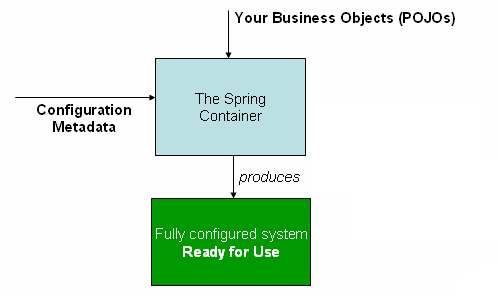
\includegraphics[width=0.8\textwidth,keepaspectratio]{container_magic}
    	\caption{Flujo de información en el contenedor de IoC}
    	\label{fig:container_magic}
    \end{figure}
    
    Existen diversas formas de especificar los metadatos de configuración. La manera original fue a través de un fichero XML, pero en la actualidad también se puede realizar con anotaciones insertadas en el código de la aplicación (añadido en la versión 2.5), o con código Java dedicado de configuración (añadido en la versión 3.0). El contenedor de IoC está completamente desacoplado de estos mecanismos de especificación de los metadatos de configuración.
    
    Existe la cuestión de qué tipo de configuración es mejor. La respuesta no es clara, ya que cada opción posee su dosis de ventajas e inconvenientes. Las anotaciones son la manera más concisa y quizás mas simple para un principiante, pero mezclan código de negocio con configuración del framework, algo que mina el principio de separación de responsabilidades. Además poseen el inconveniente de descentralizar la configuración, impactando negativamente en su mantenibilidad. La configuración con código Java permite un control centralizado, pero se pierde en facilidad y brevedad. Por su parte, los ficheros XML son inmejorables a la hora separar responsabilidades, pudiéndose alterar la configuración sin tocar una línea de código y, por tanto, sin tener que recompilar. El inconveniente de este sistema es el elevado tamaño y complejidad que muchas veces estos ficheros alcanzan, siendo además su curva de aprendizaje más pronunciada.
    
    En el desarrollo de la presente aplicación web se ha utilizado la configuración a través de anotaciones y de código Java dedicado. Además, se ha utilizado Spring Boot, lo que, como se verá, implica que una gran parte (la mayoría) de la configuración necesaria ha sido establecida por defecto.
    \\
    
    Además del contenedor de IoC, la aplicación web desarrollada hace uso de otras capacidades ofrecidas por Spring Framework:
    
    \begin{itemize}
    	\item[-] Publicación y escucha de eventos.
    	\item[-] Gestión de transacciones.
    	\item[-] Planificación de tareas.
    	\item[-] Validación.
    	\item[-] El framework de desarrollo web \emph{Spring Web MVC} (comúnmente conocido como simplemente Spring MVC).
    \end{itemize}
    
    Spring MVC, como muchos otros frameworks de desarrollo web, está implementado alineado con el patrón de diseño \emph{Front Controller}, donde un Servlet central, el llamado \emph{DispatcherServlet}, recibe las peticiones HTTP y delega su procesamiento a los componentes apropiados, en el caso de la presente aplicación los objetos anotados con \emph{@Controller}. Cada uno de estos objetos es responsable de llevar a cabo las acciones necesarias para cada \emph{endpoint} expuesto, apoyándose para ello en la capa de negocio, es decir, en los objetos anotados con \emph{@Service}. Como ya se explicó en la sección \ref{sec:design_layer}, estos objetos \emph{@Service} se apoyan, a su vez, en otros objetos de su clase y en objetos anotados con \emph{@Repository}, que actúan como puerta de entrada a los datos. Cumplida la lógica de negocio, el objeto \emph{@Controller} implicado devuelve el nombre de la vista a proporcionar como respuesta, así como los datos con los que poblarla. El motor de plantillas genera en este punto el contenido HTML, que es devuelto por el \emph{DispatcherServlet} al usuario.
    
    En resumen, Spring MVC ofrece la infraestructura \emph{Front Controller}, esto es, los objetos necesarios para resolver el mapeo de las peticiones HTTP a los métodos apropiados de los objetos \emph{@Controller}, los objetos encargados de resolver las vistas, los encargados del enlace de datos, etc, permitiendo al desarrollador centrarse en especificar la lógica de negocio.
    
    \paragraph{Spring Boot}
    Este proyecto ha sido el gran avance de los últimos años dentro del universo Spring. De hecho, ha cambiado por completo el paradigma, permitiendo el desarrollo de aplicaciones totalmente funcionales en un espacio de tiempo dramáticamente inferior al necesario con anterioridad a su aparición. Tal como viene recogido en la \href{https://docs.spring.io/spring-boot/docs/current-SNAPSHOT/reference/html/}{documentación} oficial, sus principales objetivos son:
    
    \begin{itemize}
    	\item[-] Ofrecer una vía de entrada al uso de las tecnologías Spring radicalmente más rápida y sencilla.
    	\item[-] Proporcionar una configuración por defecto sensata, y al mismo tiempo de ágil modificación si los requisitos así lo necesitan.
    	\item[-] Ofrecer todo un abanico de funcionalidades transversales a la mayoría de aplicaciones, como los servidores embebidos.
    	\item[-] Supresión de la necesidad de configuración a través de ficheros XML.
    \end{itemize}
    
    Así, Spring Boot no es una alternativa a otros proyectos Spring. Su objetivo no es proporcionar nuevas soluciones para problemas ya resueltos, sino ofrecer una manera de mejorar el aprovechamiento del ecosistema entero, fomentando una experiencia de desarrollo que simplifique el uso de los módulos ya disponibles. Esto hace que Spring Boot sea una opción ideal para toda clase de desarrolladores, tanto los que ya están familiarizados con el ecosistema Spring como aquellos recién llegados, al permitirles adoptar las tecnologías de Spring de una manera simplificada. En este sentido, Spring Boot ha supuesto un vector de expansión de las tecnologías Spring, disminuyendo su barrera de entrada y maximizando el aprovechamiento de sus variadas funcionalidades.
    
    En gran medida, lo expuesto se consigue gracias a que Spring Boot ejercita el paradigma de diseño conocido como Convención sobre Configuración (\emph{Convention over Configuration, CoC}), o también como Código por Convención (\emph{Coding by Convention}). Este principio de diseño trata de disminuir el número de decisiones que el desarrollador debe tomar y aliviar así la complejidad de tener que configurar todas y cada una de las áreas que conforman una aplicación, todo ello sin necesariamente merma alguna en la flexibilidad. Así, el desarrollador sólo está llamado a especificar los aspectos no convencionales de la configuración de la aplicación, obteniendo como resultado inmediato un aumento en la productividad considerable.
    
    Conviene destacar también que Spring Boot permite ejecutar aplicaciones web sin necesidad de hacerlo en un contenedor de servlets externo o un servidor de aplicaciones, ya que el propio Spring Boot incluye un Tomcat embebido, el cual se despliega automáticamente en tiempo de ejecución.
    
    \paragraph{Spring Data JPA - Hibernate ORM}
    El proyecto Spring Data JPA, parte de la amplia familia Spring Data, es una capa de abstracción extra sobre la implementación de la especificación JPA que se utilice, que en el caso del presente proyecto ha sido Hibernate ORM.
    
    Por persistencia se hace referencia a la funcionalidad que permite que determinados objetos creados por la aplicación puedan sobrevivir más allá de la frontera de la misma. En términos Java, se trata de que el estado de ciertos objetos pueda perdurar fuera del entorno de la JVM, de modo que dicho estado esté disponible en cualquier momento posterior.
    
    \begin{figure}[hbt!]
    	\centering
    	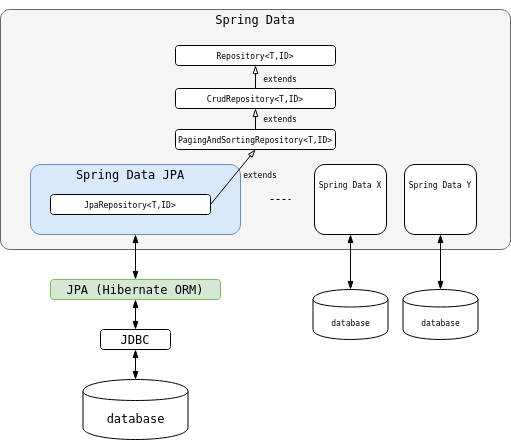
\includegraphics[width=\textwidth,keepaspectratio]{data_access}
    	\caption{Esquema de la infraestructura de acceso a datos}
    	\label{fig:data_access}
    \end{figure}
    
    JPA es una especificación que define una API de mapeo objeto-relacional y gestión de objetos persistentes. Además, hace innecesario el tratamiento explícito de las conexiones/recursos usuales al trabajar directamente con JDBC. Actualmente se encuentra en su versión 2.2, siendo su implementación de referencia EclipseLink. No obstante, Spring usa por defecto Hibernate ORM como proveedor de JPA, y en el presente proyecto no se ha modificado dicha configuración preestablecida.
    
    El mapeo objeto-relacional es la funcionalidad que permite la traducción entre los objetos de la aplicación (llamados entidades en este contexto) y las tablas de la base datos. Esto implica gestionar, entre otras cosas, las relaciones que existen entre las entidades. Esta es una tarea no trivial que los proyectos con necesidades de persistencia relacional (en contraposición con los modelos no relacionales, no tratados en el presente proyecto) deben afrontar. En este sentido, Hibernate ORM (Object/Relational Mapping) es un framework que permite la simplificación y en parte automatización de esta tarea. Como ejemplo, y sin entrar en detalles, las relaciones entre las entidades son especificadas a través de las anotaciones \emph{@OneToOne}, \emph{@OneToMany}, \emph{@ManyToOne} y \emph{@ManyToMany}.
    
    Resaltar que además del mapeo objeto-relacional, la abstracción JPA ofrece (de la mano de Hibernate ORM, en este caso) la gestión del ciclo de vida de las entidades y el lenguaje de consultas relacionales orientado a objeto JPQL. En el listado \ref{list:jpql} se muestra un ejemplo de consulta con este lenguaje extraído del presente proyecto.
    
    \begin{lstlisting}[caption=Ejemplo de consulta especificada en JPQL,label=list:jpql]
    @Query("SELECT b.id FROM Book b WHERE b.publisher.id IN :publisherIds")
    Set<Long> findIdByPublisherIds(@Param("publisherIds") Set<Long> publisherIds);
    \end{lstlisting}
    
    En este punto, vistas las capacidades de abstracción que ofrece JPA a través de sus implementaciones, cabe preguntarse porqué añadir otra capa de abstracción encima con Spring Data JPA. La respuesta es que esta tecnología añade aún más facilidades de desarrollo y mantenimiento, en concreto:
    
    \begin{itemize}
    	\item[-] Permite la integración de JPA con el ecosistema Spring de una forma natural.
    	\item[-] Permite la adopción del patrón de diseño \emph{Repositorio} (ver sección \ref{sec:design_layer}) sin necesidad de añadir código extra, ya que Spring Data JPA, como subconjunto de Spring Data, proporciona una serie de interfaces al efecto, tal como se esquematiza en la figura \ref{fig:data_access}. Así, construir una interfaz repositorio para cualquier entidad de la aplicación es tan fácil como extender alguna de las proporcionadas. En el presente proyecto todos los repositorios extienden a \emph{CrudRepository\textless{}T,ID\textgreater{}}.
    	\item[-] Además de ofrecer las interfaces, también lo hace con sus implementaciones. Es decir, el desarrollador puede olvidarse de crear código que implemente las interfaces de acceso a datos, Spring Data JPA lo realiza automáticamente.
    	\item[-] Posibilidad de inferir las consultas de acceso a datos a partir del nombre del método en la interfaz. Esta funcionalidad ha sido usada extensamente en el desarrollo del presente proyecto. En el listado \ref{list:query_inference} se muestra un método de la interfaz \emph{SecurityTokenRepository}, a partir del cual Spring Data JPA construye la consulta necesaria para obtener los \emph{SecurityToken} que cumplan estar asociados a un usuario determinado, con un \emph{SecurityEvent} dado y creados después de un punto temporal dado.
    \end{itemize}
    
    \begin{lstlisting}[caption=Ejemplo de método a partir del cual Spring Data JPA infiere la consulta apropiada,label=list:query_inference]
    Set<SecurityToken> findByTargetUserAndSecurityEventAndCreatedDateAfter(User targetUser, SecurityEvent securityEvent, LocalDateTime dateTime);
    \end{lstlisting}
    
    En resumen, Spring Data JPA añade una capa de abstracción sobre JPA, lo que significa que hace uso de todas las funcionalidades que esta especificación proporciona, y además suministra sus propias facilidades, como la implementación sin código del patrón \emph{Repositorio} o la creación de consultas a la base datos a partir del nombre de los métodos.
    
    \subsubsection{Thymeleaf} \label{sec:thymeleaf}
    Thymeleaf es un motor de plantillas para aplicaciones Java, tanto web como de escritorio, que permite crear dinámicamente documentos HTML5 (y otros, como XML o XHTML). Como principales características de esta tecnología cabe resaltar:
    
    \begin{itemize}
    	\item[-] Thymeleaf ejercita el concepto llamado \emph{natural templating}, esto es, las propias plantillas son documentos HTML5 válidos, de forma que prácticamente cualquier navegador las puede renderizar, mostrando su contenido por defecto. Esto es muy útil en la fase de desarrollo de la aplicación, ya que no hay necesidad de contar con un contenedor web para visualizar el resultado de la plantilla (como ocurre con la tecnología JSP), facilitando el trabajo paralelo sobre una misma vista en las labores frontend y backend.
    	\item[-] Es altamente extendible. Cualquiera puede crear su propio conjunto de atributos o etiquetas, con los nombres que se desee, definir sintaxis para expresiones y su lógica de evaluación, etc. Esto es, es posible crear lo que se denominan \emph{dialectos} de Thymeleaf, actuando así esta tecnología como un framework de plantillas. Por defecto se usa el conocido como dialecto \emph{Standard}.
    	\item[-] Thymeleaf se integra con muchísima facilidad con la tecnología Spring. De hecho, desde Spring se recomienda preferentemente su uso. Así, se dispone de un dialecto propio: el \emph{SpringStandard}, el cual permite el uso de Spring Expression Language. La integración con Spring Security es muy sencilla, permitiendo acoplar lógica de autenticación y/o autorización en las plantillas de una manera muy poco intrusiva.
    \end{itemize}
    
    En el presente proyecto, los documentos incorporados en \emph{classpath: resources/templates} son las plantillas HTML que el motor toma, junto con los datos de negocio que Spring MVC le suministra, para producir el contenido HTML5 que se sirve al cliente.
    
    \subsubsection{Bootstrap}
    En el ámbito del diseño frontend de la presente aplicación, la herramienta que más ha destacado a sido Bootstrap, versión 4. Se trata de un framework de HTML, CSS y JavaScript, que prima el desarrollo \emph{responsive}. Esto quiere decir que la aplicación web adapta su presentación al tamaño de la pantalla disponible, esto es, que \emph{responde} automáticamente a los cambios de tamaño de pantalla, de forma que en cada caso optimiza la presentación.
    
    Gracias a Bootstrap, con relativamente poco esfuerzo se puede ofrecer una experiencia de usuario muy correcta. Un gran número de elementos HTML como formularios, botones, encabezados, etc. son proporcionados por este framework, con estilo CSS ya preconfigurado, además de otros elementos como \emph{spinners}, \emph{modals}, \emph{cards} etc., lo que aumenta enormemente la productividad.  Además, aparte de los objetos, Bootstrap permite controlar el layout de las vistas de una manera muy sencilla y potente, basada en los Flexbox de CSS.
    
    Cuando el framework no es capaz de ofrecer una funcionalidad siempre se pueden usar directamente hojas de estilo CSS3, como ha sido el caso en el presente proyecto en varias ocasiones (\emph{classpath: resources/static/css/fmstyle.css}). Además, se han utilizado otros componentes que merecen especial mención:
    
    \begin{itemize}
    	\item[-] \href{https://fontawesome.com/}{FontAwesome}. Todos los iconos mostrados en la aplicación web han sido obtenidos de FontAwesome.
    	\item[-] \href{https://lokesh-coder.github.io/pretty-checkbox/}{Pretty Checkbox}. Con el objetivo de dar un mejor aspecto a los \emph{check boxes} utilizados, respecto del ofrecido por Bootstrap, se decidió usar esta librería CSS.
    	\item[-] \href{https://fonts.google.com/}{Google Fonts}. A efectos de dar un cariz más personalizado a la aplicación web se usó este servicio de Google. La fuente usada en la aplicación web ha sido \href{https://fonts.google.com/specimen/Noto+Serif+JP}{Noto Serif JP}.
    \end{itemize}
    
    \subsection[Pagos con Stripe]{Gestión de Pagos con Stripe} \label{sec:stripe}
    Los comercios, ya sean presenciales u \emph{online}, son en esencia lugares de intercambio. Normalmente, lo que una de las partes ofrece a la otra es dinero, a través de un pago. Por tanto, cabe esperar que, en cualquiera de estos establecimientos, el procedimiento por el cual se materializa el pago tome un lugar especial dentro de la lógica de negocio.
    
    Los comercios en Internet tienen, además, la responsabilidad de ofrecer altos estándares de seguridad a sus clientes, especialmente en lo concerniente con el pago. De hecho, una de las principales barreras que aparta a potenciales usuarios del comercio \emph{online} es la percepción de inseguridad que el proceso de pago telemático lleva asociado. En este sentido, el comercio a través de Internet depende de una manera radical en la confianza de los usuarios, siendo así este uno de los principales capitales a cultivar y fortalecer.
    
    La percepción de inseguridad no es en absoluto infundada. El notable desarrollo de la sociedad de la información a lo largo de las últimas décadas lleva inevitablemente asociado el incremento de las modalidades y de la capacidad de fraude digital. No obstante, en una pugna continua, la tecnología anti-fraude trata de mantenerse en todo momento actualizada para ejercer de contrapeso.
    
    Así, como se ha comentado, el pago es una tarea de vital importancia, transversal a todas las plataformas de comercio, con unos estrictos requisitos de seguridad a fin de generar la confianza que demanda el mercado. Es en este contexto donde juegan un papel esencial los proveedores de servicios de pago \emph{online}.
    
    Actualmente en el mercado existen múltiples alternativas de servicios de este tipo, como \href{https://www.paypal.com/}{PayPal} o \href{https://securionpay.com/}{SecurionPay}, pero el elegido para el desarrollo del presente proyecto ha sido \href{https://stripe.com/}{Stripe}. Amén de su consolidada posición en el mercado como uno de los servicios líderes en el sector, la principal característica diferenciadora ha sido la \href{https://stripe.com/docs}{cuidada colección} de documentación, guías, ejemplos, etc. que mantienen para facilitar la integración con su infraestructura. En el resto de esta sección se comentará los detalles de dicha integración con Stripe, mientras que en la sección \ref{sec:striperadar} se hará lo propio con la funcionalidad anti-fraude que esta plataforma de pagos \emph{online} ofrece.
    \\
    
    Fundamentalmente, la aplicación web desarrollada se integra con la infraestructura de Stripe haciendo uso de dos puntos de enlace, uno en backend y otro en frontend:
    
    \begin{itemize}
    	\item[-] Una extensa interfaz de programación backend, \href{https://stripe.com/docs/api}{Stripe API}, para varios lenguajes (entre ellos Java), plena de funcionalidades que cubren multitud de casos de uso relacionados con la gestión de transacciones monetarias y sus aspectos asociados.
    	
    	La integración de la presente aplicación web se ha basado en el objeto \href{https://stripe.com/docs/api/payment_intents}{PaymentIntent}. Un PaymentIntent mantiene la información relacionada con un pago puntual. Entre dicha información, una pieza clave es el \emph{client\_secret}, que es el código identificativo de la transacción que permite al cliente, usándolo como parámetro en la invocación de funciones en \emph{Stripe.js}, finalizar el pago. Además, el PaymentIntent mantiene la información sobre la situación del pago que gestiona al recorrer una serie de \href{https://stripe.com/docs/payments/intents#intent-statuses}{estados} desde su creación (su ciclo de vida). Como se verá, FirstMarket conoce de estos estados al escuchar las notificaciones que Stripe le envía al \emph{webhook} configurado.
    	
    	\item[-] Una librería frontend, \href{https://stripe.com/docs/js}{\emph{Stripe.js}}, que permite, entre otras cosas, gestionar la comunicación entre el cliente y Stripe, y la inserción de elementos gráficos configurables en las vistas que la aplicación web sirve al cliente. Estos \href{https://stripe.com/docs/js/elements_object}{elementos} son empleados para recabar la información sensible de los formularios de pago (por ejemplo, el número de la tarjeta de débito).
    	
    	La presente aplicación web coordina todo el proceso de pago en el lado del cliente mediante el script desarrollado \emph{checkout.js}. En él, como se muestra en el listado \ref{list:js_checkout_card}, se ha usado el elemento \emph{card} ofrecido en \emph{Stripe.js}. En la figura \ref{fig:checkout_form} se muestra el resultado obtenido, siendo el citado elemento \emph{card} la entrada del formulario donde se solicita la información de la tarjeta bancaria.
    \end{itemize}
    
    \begin{lstlisting}[language=Javascript,caption=Extracto de checkout.js donde se crea y enlaza el elemento \emph{card},label=list:js_checkout_card]
    //...
    
    let stripe = Stripe(stripePublicKey);
    let elements = stripe.elements();
    let cardElement = elements.create('card');
    cardElement.mount('#card-element');
    
    //...
    \end{lstlisting}
    
    \begin{figure}[hbt!]
    	\centering
    	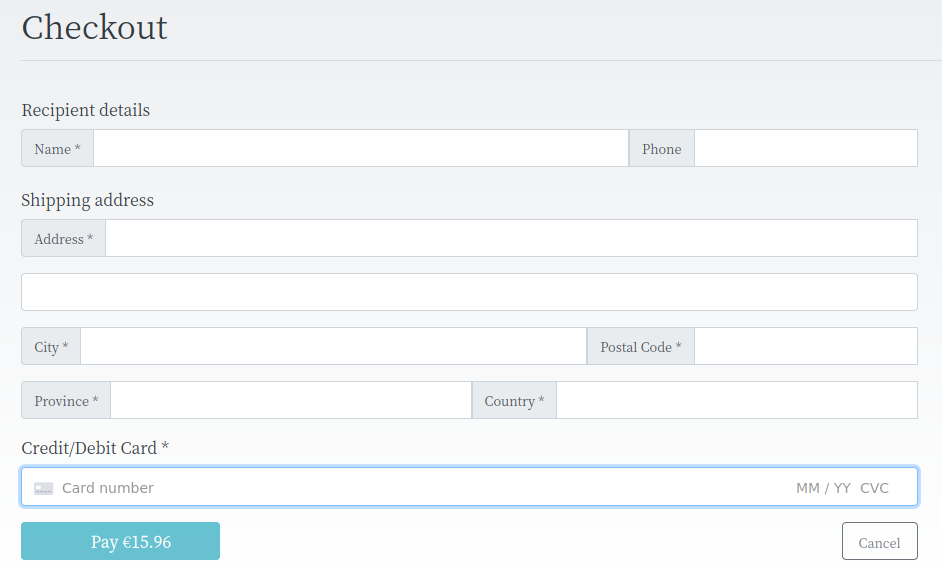
\includegraphics[width=\textwidth,keepaspectratio]{checkout_form}
    	\caption{Formulario de checkout}
    	\label{fig:checkout_form}
    \end{figure}
    
    \begin{figure}[hbt!]
    	\centering
    	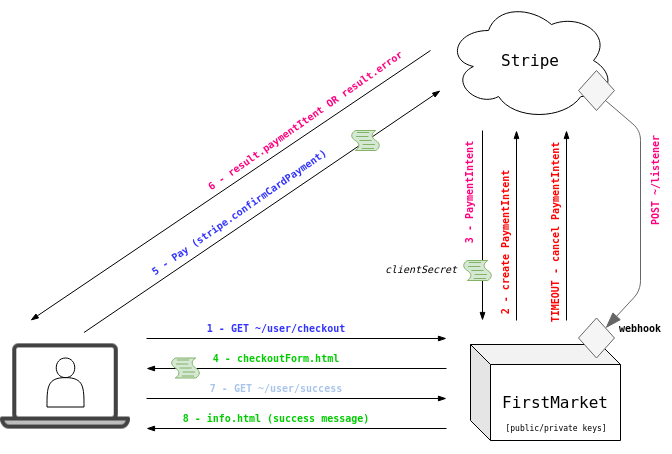
\includegraphics[width=\textwidth,keepaspectratio]{stripe}
    	\caption{Flujo de información durante un pago}
    	\label{fig:stripe}
    \end{figure}
    
    Una vez se ha comentado todo lo anterior, se está en disposición de esbozar el flujo de información que tiene lugar durante el proceso de pago, tomando como apoyo el esquema presentado en la figura \ref{fig:stripe}:
    
    \begin{itemize}
    	\item[1.] El cliente, estando en la vista de su cesta, decide proceder a finalizar la compra y hace click en el botón de ckeckout. Esto se traduce en una petición a FirstMarket al \emph{endpoint} GET \nolinkurl{~/user/checkout}. 
    	\item[2.] Tal como se explica en \ref{sec:concurrencia}, el sistema comprueba la disponibilidad de los libros pedidos y, si es el caso, compromete la cesta. En el proceso de comprometer la cesta contacta con Stripe para crear el PaymentIntent, especificando en este punto, entre otras cosas, la cantidad exacta a cobrar.
    	\item[3.] Stripe devuelve al sistema el PaymentIntent recién creado, el cual contiene el \emph{client\_secret}.
    	\item[4.] El sistema sirve la vista \emph{checkoutForm.html} al cliente, la cual lleva inserta el \emph{client\_secret}. Resaltar en este punto la importancia del encriptado que protocolos de transporte seguro proporcionan, ya que este código sólo debe ser conocido, fuera de Stripe y de Firstmarket, por el cliente. Así, como se explica en la sección \ref{sec:https}, la aplicación web desarrollada emplea HTTPS.
    	\item[5.] Tras completar correctamente el formulario de checkout (presentado en la figura \ref{fig:checkout_form}), el cliente presiona el botón de pagar. Esto desencadena que desde \emph{checkout.js} se invoque la función \emph{confirmCardPayment} (perteneciente a la librería \emph{Stripe.js}), tomando como parámetro, entre otros valores, el \emph{client\_secret}.
    	\item[6.] Stripe procesa el pago y responde al cliente enviándole el objeto \emph{result} (más adelante se explicará que en este punto, y en otros, Stripe notifica a FirstMarket a través del \emph{webhook}). Dependiendo del éxito o no del pago, este objeto contendrá en su interior, respectivamente, el PaymentIntent o un objeto \emph{error}. En ambos casos, \emph{checkout.js} toma las medidas oportunas. En caso de éxito, se realiza lo explicado en el siguiente punto. En caso contrario se notifica por pantalla al cliente para que tome las medidas oportunas.
    	\item[7.] \emph{checkout.js} realiza en background una petición a FirstMarket al \emph{endpoint} GET \nolinkurl{~/user/success}.
    	\item[8.] El sistema sirve la vista \emph{info.html} al cliente, la cual le comunica que el pedido se ha realizado con éxito y que pronto recibirá confirmación por email.
    \end{itemize}
    
    Notar en la figura \ref{fig:stripe} que, tal como se explicó en la sección \ref{sec:concurrencia}, cuando se produce el \emph{timeout} y el pago no se ha efectuado se activa la vía de descomprometer la cesta y, por tanto, cancelar el PaymentIntent.
    
    Por otro lado, podría pensarse que FirstMarket conoce de la finalización con éxito del pago a través de la solicitud que en el punto 7 anterior el cliente le realiza. Sin embargo, esa solicitud sólo es usada en backend como disparador para servir el mensaje estándar de finalización de una compra. Es decir, el sistema no realiza ninguna acción de lógica de negocio (no crea ningún pedido, de modifica ninguna cesta, etc.) al recibir la petición del punto 7. Sólo se limita a servir una vista con un mensaje. De hecho, cualquier cliente con sesión abierta en FirstMarket puede escribir en su navegador la dirección \nolinkurl{~/user/success} y el sistema le devolverá el mensaje de compra finalizada (por supuesto, sin haber realizado ninguna compra en realidad).
    
    Esto es así porque para conocer del estado de un pago FirstMarket no debe depender del cliente, sino de Stripe directamente. Y esta comunicación directa se realiza por medio del \emph{webhook} configurado en Stripe. Esto es, Stripe permite configurar el envío de notificaciones POST ante los eventos que se desee, existiendo multitud de \href{https://stripe.com/docs/api/events/types}{eventos disponibles}. FirstMarket escucha notificaciones POST provenientes de Stripe (se comprueba que es Stripe quien notifica al comparar la dirección IP de origen con las \href{https://stripe.com/docs/ips}{oficiales} de Stripe, además de por existir un código de verificación en las notificaciones) en el \emph{endpoint} \nolinkurl{~/listener}. En concreto, se ha configurado la notificación de los eventos relacionados con el ciclo de vida de los PaymentIntent:
    
    \begin{itemize}
    	\item[-] \emph{payment\_intent.succeeded}. El pago ha concluido con éxito. Es al recibir esta notificación cuando el sistema realiza las acciones necesarias de lógica de negocio para, por ejemplo, crear el nuevo pedido.
    	\item[-] \emph{payment\_intent.canceled}. El PaymentIntent ha sido cancelado. Se procede, si fuese necesario, a descomprometer la cesta.
    	\item[-] \emph{payment\_intent.payment\_failed}. Ocurre cuando el pago ha fallado. No se realiza ninguna acción aparte de su registro.
    	\item[-] \emph{payment\_intent.created}. El PaymentIntent ha sido creado. No se realiza ninguna acción aparte de su registro.
    	\item[-] \emph{payment\_intent.processing}. Ocurre cuando el PaymentIntent ha comenzado su procesamiento. No se realiza ninguna acción aparte de su registro.
    	\item[-] \emph{payment\_intent.amount\_capturable\_updated}. Se da cuando el PaymentIntent posee fondos aún por capturar. No se realiza ninguna acción aparte de su registro.
    \end{itemize}
    
    La principal consecuencia de la arquitectura explicada es que \textbf{FirstMarket nunca tiene contacto con la información sensible del cliente}. Esta se envía directamente a Stripe desde el cliente. Las implicaciones en términos de seguridad de este aspecto son profundas, mejorándose la exposición al riesgo de los clientes al tiempo que se alivian los requisitos y el coste de la aplicación web. De hecho, todo agente involucrado en el procesamiento, transmisión o almacenamiento de datos bancarios sensibles debe cumplir con los estándares del \href{https://www.pcisecuritystandards.org/pci_security/}{\emph{Payment Card Industry Security Standards Council}}. En este sentido, Stripe ha sido certificado como \emph{PCI Level 1 Service Provider}, el nivel de certificación más estricto disponible en la industria de pagos. Por su parte, Firstmarket se alinea con los estándares PCI al no tener relación, como se ha dicho, con la información sensible de los clientes, y al garantizar la utilización de TLS en sus comunicaciones.
    \\
    
    Como último apunte, Stripe no es gratis. Su modelo de negocio se basa en cobrar una comisión por cada transferencia que procesa. Para identificar a cada comercio ofrece un par de llaves, una pública y otra privada. Además, para facilitar las labores de desarrollo software, proporciona dos juegos de estas llaves: unas para \emph{test} y otras \emph{live}. Como su nombre indica, las primeras pueden ser usadas durante las labores de testeo de la integración, pudiendo simularse transacciones usando los datos de \href{https://stripe.com/docs/payments/accept-a-payment#web-test-integration}{tarjetas bancarias ficticias} ofrecidas por Stripe. El juego de llaves \emph{live}, por su parte, permite realizar pagos reales. Sin embargo, dada la política de Stripe para el control de blanqueo de capitales, para activar este juego de llaves se debe presentar la documentación oficial de la constitución de la persona jurídica que recibe los pagos. Es por ello que en el presente proyecto sólo se ha empleado el juego de llaves \emph{test}, aceptando únicamente transacciones simuladas. En la figura \ref{fig:stripe_dashboard} se muestra el \emph{dashboard} de Stripe, desde donde es posible controlar todo lo referente a la integración con esta plataforma. Se puede apreciar el requerimiento para proveer la información legal necesaria para desbloquear las llaves \emph{live}.
    
    \begin{figure}[hbt!]
    	\centering
    	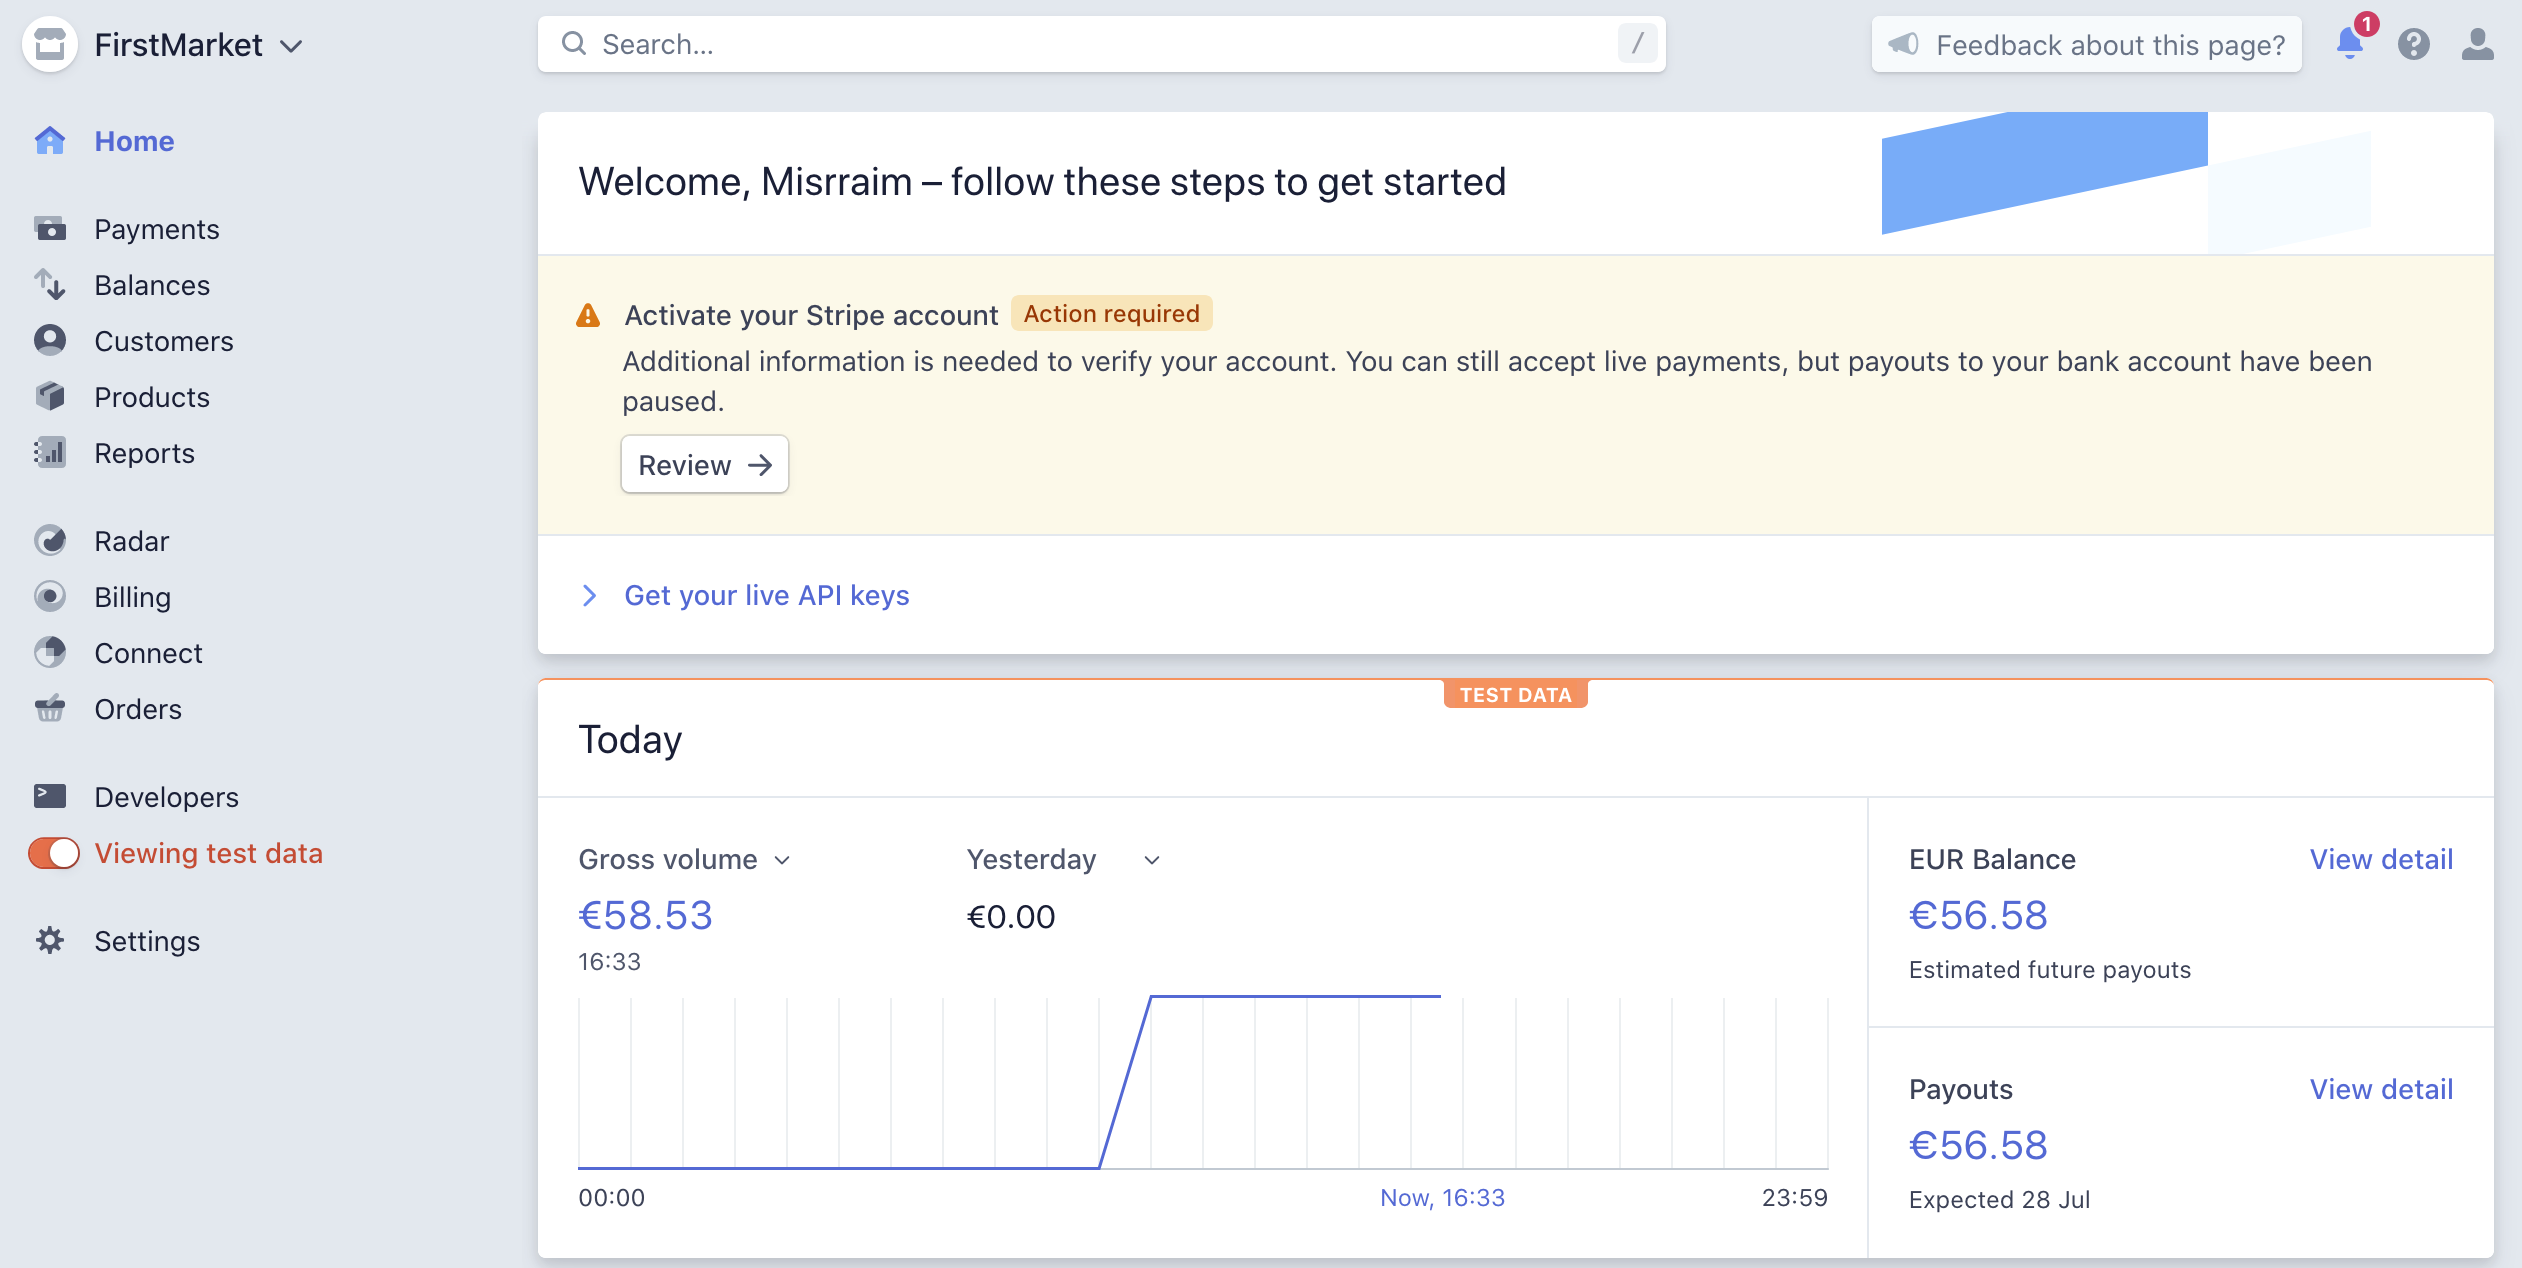
\includegraphics[width=\textwidth,keepaspectratio]{stripe_dashboard}
    	\caption{Stripe Dashboard}
    	\label{fig:stripe_dashboard}
    \end{figure}
    
    \subsection{Control de Concurrencia} \label{sec:concurrencia}
    Uno de los aspectos más críticos para el correcto funcionamiento de una tienda online es el control del stock de productos y del proceso de realización de una compra. Muchos usuarios, quizás simultáneamente, pueden añadir productos a sus cestas y proceder a su compra. La aplicación debe garantizar que estas acciones se realicen de forma a conservar en todo momento la consistencia de los datos.
    
    \begin{figure}[hbt!]
    	\centering
    	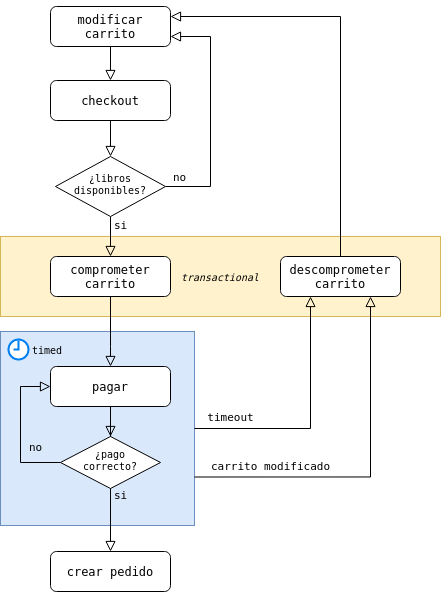
\includegraphics[width=0.7\textwidth,keepaspectratio]{cart_concurrent}
    	\caption{Diagrama del proceso de finalización de una compra}
    	\label{fig:cart_concurrent}
    \end{figure}
    
    Como se puede apreciar en la figura \ref{fig:cart_concurrent}, cuando un usuario decide proceder con el pedido de los libros contenidos en su cesta, lo primero que hace el sistema es comprobar que esos libros están disponibles. Pueden no estarlo por dos motivos, a saber, que estén agotados en ese momento o que el administrador de la aplicación web los haya deshabilitado (además, en este último caso el sistema automáticamente retira de la cesta dichos libros al detectar dicha situación). Si alguno de estos escenarios ocurriese la aplicación informaría al usuario en la propia vista de la cesta, sin avanzar a la vista de checkout, tal como se muestra en la figura \ref{fig:cart_alert}.
    
    \begin{figure}[hbt!]
    	\centering
    	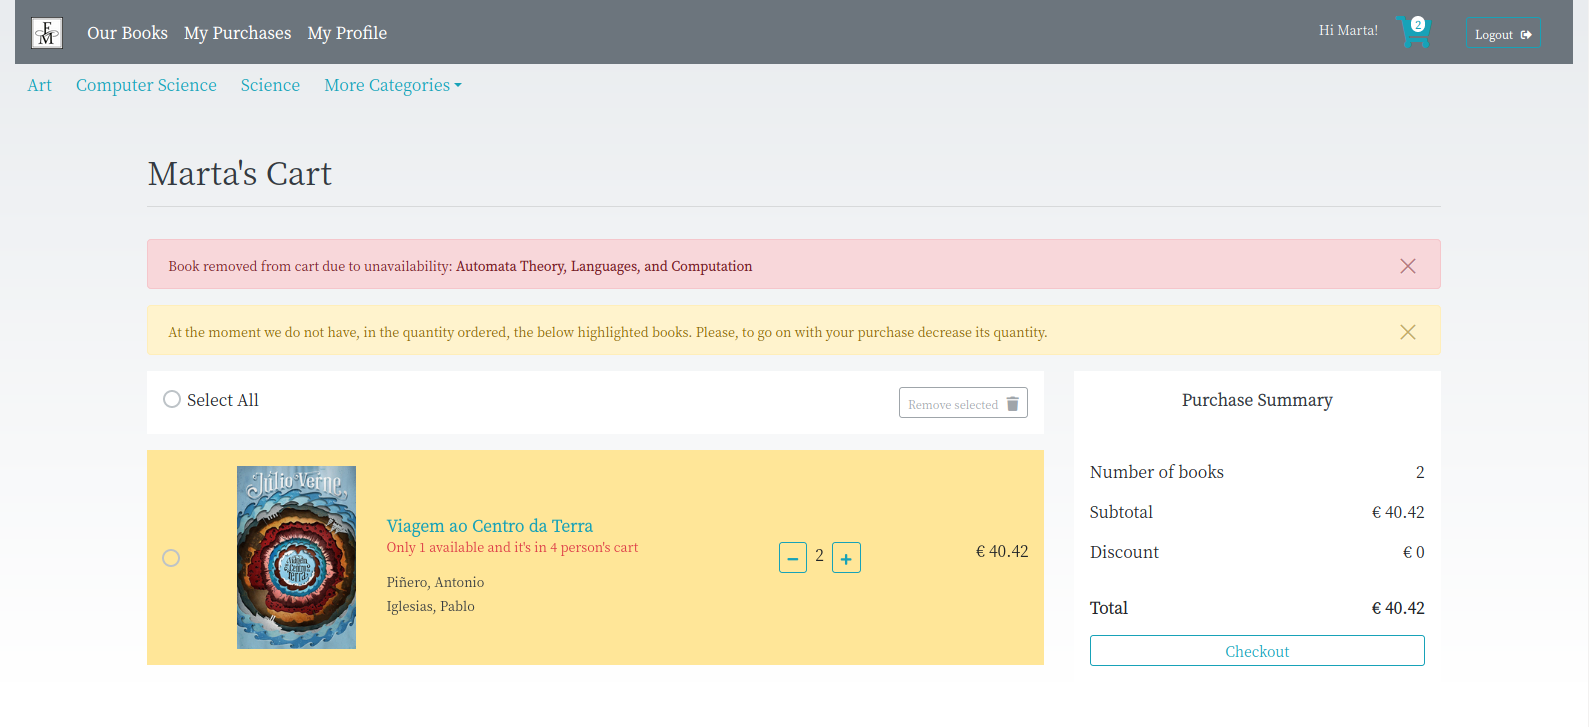
\includegraphics[width=\textwidth]{cart_alert}
    	\caption{Aviso por pantalla de no disponibilidad de libros}
    	\label{fig:cart_alert}
    \end{figure}
    
    Tras comprobar que los libros están disponibles el sistema \textbf{compromete} la cesta. Este es el paso fundamental donde se garantiza la consistencia. El sistema se compromete con el usuario a que si este finaliza la compra (dentro de un tiempo establecido) se le entregarán los libros seleccionados y al precio actual. Internamente, lo más destacado que el sistema realiza se recoge en:
    
    \begin{itemize}
    	\item[-] Se actualiza el stock, sustrayendo los libros en las cantidades correspondientes.
    	\item[-] Se crea en la base de datos una entidad \emph{sale} por cada item de la cesta, para así capturar el estado (principalmente el precio) de los libros en ese momento.
    	\item[-] Se contacta con Stripe para crear un nuevo \emph{Payment Intent}.
    	\item[-] Se activa el contador de tiempo disponible para finalizar la compra.
    \end{itemize}
    
    Todas estas acciones que realiza el sistema para comprometer la cesta las lleva a cabo de forma transaccional, apoyándose en la API de Spring Data JPA (ver \ref{sec:spring}). Las transacciones software se describen en términos de las características ACID, del acrónimo en inglés de Atomicity, Consistency, Isolation, y Durability:
    
    \begin{itemize}
    	\item[-] Atomicity. Cada paso en la secuencia de acciones realizadas dentro de los límites de una transacción deben completarse con éxito o todo el trabajo debe
    	retroceder. La finalización parcial no es posible, o sucede todo o no sucede nada.
    	\item[-] Consistency. Los recursos de un sistema deben estar en un estado coherente, no corrupto, tanto en el inicio como en la finalización de una transacción.
    	\item[-] Isolation. El resultado de una transacción no debe ser visible para otras transacciones hasta que la primera se confirme con éxito.
    	\item[-] Durability. El resultado de una transacción comprometida debe hacerse permanente, independientemente a cualquier fallo del sistema.
    \end{itemize}
    
    Una vez comprometida la cesta, que otro usuario modifique el stock (ya sea un cliente al comprar un libro o el administrador al variar el stock), o que el administrador varíe el precio de algún libro de los recién comprometidos, o que incluso deshabilite alguno de estos libros, sería transparente para el usuario que acaba de comprometer su cesta. Mientras dure el tiempo disponible para finalizar la compra, la cesta comprometida es un contrato inmodificable. En este punto pueden suceder dos cosas: 
    
    \begin{enumerate}
    	\item El usuario completa el formulario de checkout y paga correctamente dentro del plazo, en cuyo caso se tramitaría el nuevo pedido.
    	\item El tiempo disponible para finalizar el pago se agota sin haber sido realizado, o el usuario, en la vista de la cesta, modifica las cantidades de los libros. Ante ambos eventos el sistema procede a \textbf{descomprometer} la cesta, abortándose de facto la compra.
    \end{enumerate}
    
    El procedimiento de descomprometer la cesta es el inverso al de comprometerla, y también se realiza transaccionalmente. Así, lo más destacado que el sistema lleva a cabo internamente en este proceso se resume en:
    
    \begin{itemize}
    	\item[-] Se actualiza el stock, aumentando los libros en las cantidades correspondientes.
    	\item[-] Se eliminan las entidades \emph{sale} correspondientes de la base de datos.
    	\item[-] Se contacta con Stripe para cancelar el \emph{Payment Intent}.
    \end{itemize}

    \subsection[Datos Jerárquicos]{Persistencia y Visualización de Datos Jerárquicos} \label{sec:hierarchy}
    Desde muy pronto se reparó en la necesidad de gestionar en la base de datos información con relaciones de jerarquía, ya que las categorías de los libros están organizadas de esta manera. Además, si se implementase la funcionalidad de que los usuarios pudiesen añadir comentarios a los libros, con capacidad de respuestas anidadas, también se estaría en el escenario de estructuras jerárquicas.
    
    Tal como se explica con detalle en [bib ref], existen diversas formas de dar solución a esta necesidad, cada una de ellas con sus puntos fuertes y sus debilidades. La idoneidad de una solución frente a otra viene en gran medida determinada por la cantidad de información jerárquica a gestionar y por la frecuencia o importancia relativa de las operaciones de lectura, creación, actualización y eliminación.
    
    Si los datos jerárquicos son siempre de pequeño tamaño y las operaciones son principalmente de lectura, una solución sería cargarlos en memoria principal y gestionarlos desde allí con alguna estructura de datos apropiada. Este podría argumentarse que es el caso de la información de las categorías de los libros, ya que en principio estas no superarían a lo sumo algunas decenas de centenas, y la actividad principal realizada sería la lectura. La frecuencia con que el administrador de la tienda crea, modifica o elimina una categoría es despreciable respecto de la frecuencia con que las categorías son leídas por los usuarios en general.
    
    Por otro lado, si se implementase la funcionalidad de los comentarios anidados, el escenario es claramente diferente. La cantidad de información es potencialmente mucho mayor, con lo que trabajar directamente en memoria principal no es una opción. Además, las operaciones de creación, modificación y eliminación cobran mayor protagonismo.
    
    La solución más común en este caso se conoce como listas de adyacencia, y no es otra cosa que añadir a cada entidad una referencia (clave extranjera) al id de su predecesor jerárquico. El problema de esta solución es que escala muy mal a medida que aumenta la profundidad del árbol. Imagínese que se tiene un hilo de comentarios arbitrariamente profundo, el cual precisaría de consultas recurrentes por cada nivel si se pretendiera extraer todo el hilo (algo habitual en estos sistemas de comentarios), ya que a priori se desconoce la profundidad. Sin embargo, existen métodos para extraer todo el hilo de comentarios con una sola consulta (en general, extraer cualquier subárbol), como se verá a continuación.
    
    La funcionalidad de que los libros estén clasificados por categorías es imprescindible para la aplicación, y en consecuencia ha sido implementada. No es el caso de los comentarios. No obstante, en un intento de hacer la aplicación fácilmente ampliable en este sentido, y dado que se trata de un proyecto académico, se optó por una solución que fuese eficiente y versátil: la denominada \textbf{Closure Table}.
    
    La idea principal es mantener la información de las relaciones entre las entidades en una tabla diferente. Es decir, por una parte se encuentra la tabla \emph{category} y por otra la tabla \emph{catpath}. En la primera se almacena la información relativa a las categorías (su id, nombre, etc), mientras que en la segunda se almacena la información de los caminos en el árbol de categorías. De todos los caminos, incluso de una categoría consigo misma. Así, por cada fila en la tabla \emph{catpath} se tiene el identificador del ancestro (clave extranjera de la tabla \emph{category}), el identificador del descendiente (también clave extranjera de la tabla \emph{category}) y el tamaño del camino. Para una relación de una categoría consigo misma el tamaño del camino es 0, para una relación directa el tamaño es 1, abuelo-nieto es 2 y así sucesivamente.
    
    \begin{figure}[htb!]
    	\centering
    	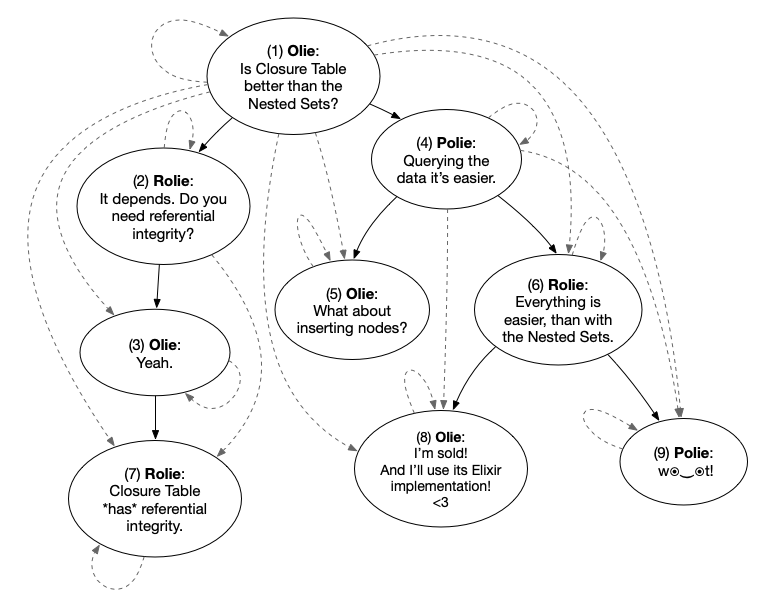
\includegraphics[width=0.7\textwidth]{closure_table}
    	\caption{Diagrama de conexiones registradas en una closure table}
    	\label{fig:closure_table}
    \end{figure}
    
    Esta solución es la más versátil y rápida de todas las mostradas en [bib ref], permitiendo incluso a un nodo pertenecer a varios árboles. Sin embargo, estos beneficios los consigue a costa de espacio. Este consumo puede ser importante si la estructura almacena jerarquías muy profundas.
    \\
    
    No obstante todo lo discutido con anterioridad, la solución real implementada para el trato específico de las categorías es triple (ver listado \ref{list:sql_cat}): Closure table, lista de adyacencia y trabajo en memoria principal con una estructura de datos en árbol. Esto es así por una cuestión de eficiencia y por desarrollar experiencia en el uso de estas soluciones.
    \\
    
    \begin{lstlisting}[caption=Tablas que gestionan las categorías,label=list:sql_cat]
    create table category (
    	id bigint not null, 
    	created_by varchar(255), 
    	created_date timestamp, 
    	last_modified_by varchar(255), 
    	last_modified_date timestamp, 
    	name varchar(255), 
    	parent_id bigint, 
    	primary key (id)
    );
    	
    create table catpath (
    	id bigint not null, 
    	created_by varchar(255), 
    	created_date timestamp, 
    	last_modified_by varchar(255), 
    	last_modified_date timestamp, 
    	size integer not null, 
    	ancestor_id bigint, 
    	descendant_id bigint, 
    	primary key (id)
    );
    
    alter table category 
    	add constraint fk_parentIdOnCategory foreign key (parent_id) references category(id)
    ;
    
    alter table catpath 
    	add constraint fk_ancestorIdOnCatpath foreign key (ancestor_id) references category(id)
    ;
    
    alter table catpath 
    	add constraint fk_descendantIdOnCatpath foreign key (descendant_id) references category(id)
    ;
    \end{lstlisting}
    
    Aparejado con el problema descrito en los párrafos anteriores se encuentra el de presentar al usuario dicha información jerárquica. Muy al principio del desarrollo de este proyecto se utilizó la tecnología de plantillas Java Server Pages para general el contenido HTML, la cual permite insertar en las vistas código Java de servidor. Así, se desarrolló una vista que contenía una función recursiva que permitía generar código HTML que mostrase la estructura anidada de las categorías. Pero esta aproximación de mezclar HTML y código Java de servidor es considerada una mala práctica y está en desuso.
    
    Posteriormente se adoptó el uso de Thymeleaf como motor de plantillas (ver \ref{sec:thymeleaf}), que no contempla esta posibilidad de insertar código de servidor en las vistas (al menos de la manera tan natural como lo permite JSP). Thymeleaf permite generar contenido lineal (una lista, por ejemplo) haciendo uso de la directiva \emph{th:each}, que hace las veces de bucle \emph{for}, pero para generar contenido anidado no dispone de ninguna funcionalidad nativa.
    
    Por todo lo anterior, para resolver este problema se optó por desarrollar código JavaScript (\emph{categoriesBuilder.js}) que se encargase, en el cliente, de construir y conectar, entre sí y al lugar apropiado en \emph{categories.html} (ver línea 15 del listado \ref{list:html_categories}), los componentes DOM necesarios para mostrar la estructura anidada de las categorías.
    \\
    
    \begin{lstlisting}[caption=Contenido principal de la vista categories.html,label=list:html_categories]
    <div class="container-fluid fm-content">
	    ...
	    <!-- main content -->
	    <div class="row">
		    <div class="col-sm-1"></div>
		    <div class="col-sm-10" id="root-hook">
			    <!-- new category -->
			    <div class="my-2 d-flex">
				    <a class="btn btn-outline-secondary align-center px-4 ml-auto" th:href="@{/admin/categoryForm}">
				    	<i class="fas fa-folder-plus fa-lg mr-4"></i>New Category
				    </a>
			    </div>
			    <hr/>
			    <!--
			    js dynamic generated content here
			    -->
		    </div>
		    <div class="col-sm-1"></div>
	    </div>
	    ...
    </div>
    \end{lstlisting}
    
    Como resultado, el administrador de la aplicación web puede visualizar la estructura jerárquica de las categorías a través de desplegables anidados, como se muestra en la figura \ref{fig:nested_categories}.
    
    \begin{figure}[htb!]
    	\centering
    	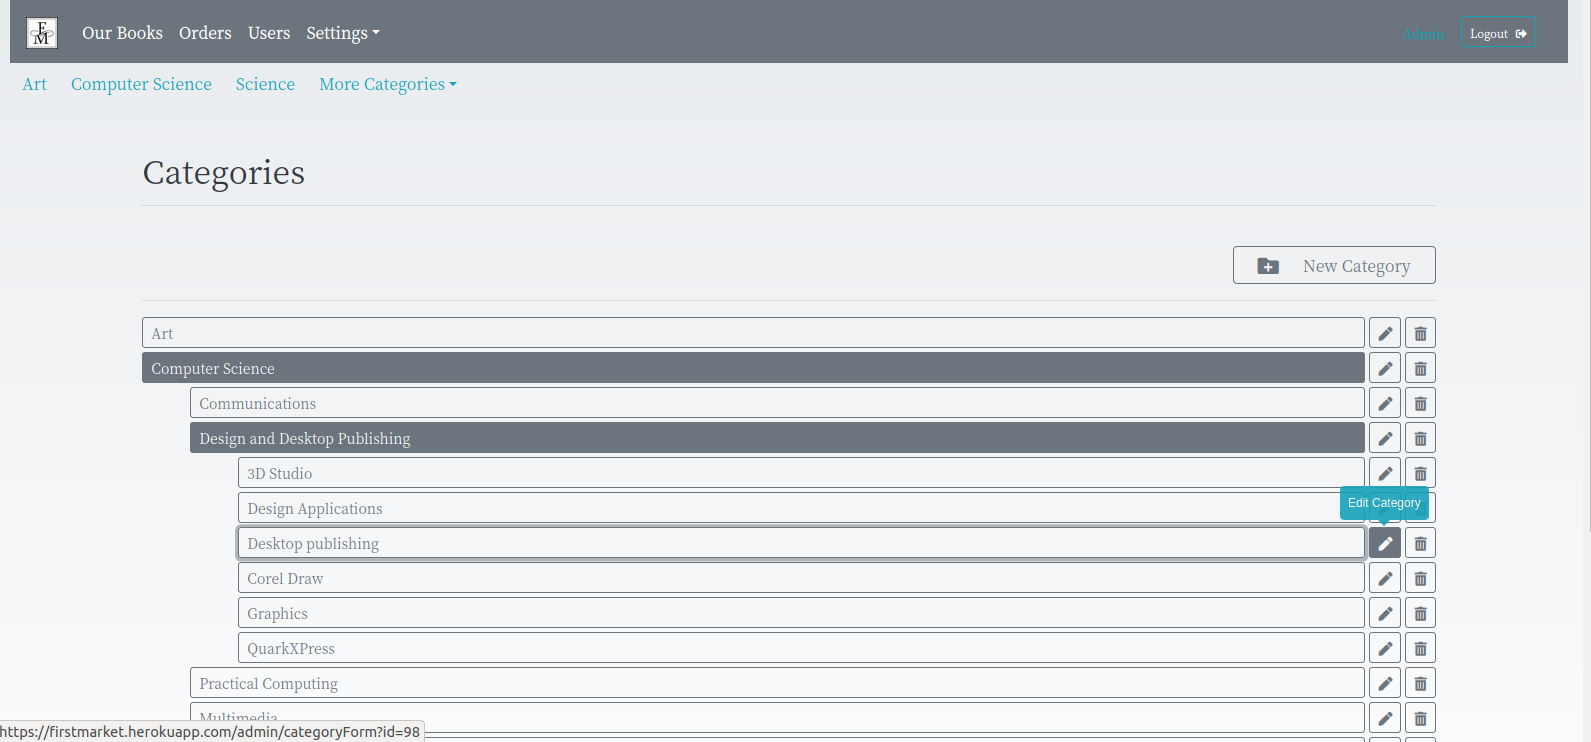
\includegraphics[width=\textwidth]{nested_categories}
    	\caption{Visualización de la estructura anidada de las categorías}
    	\label{fig:nested_categories}
    \end{figure}
    
    \subsection{Experiencia de Usuario Mejorada}
    Uno de los requisitos básicos de la aplicación web desarrollada es el de permitir a los usuarios gestionar su compra mediante el uso de una cesta virtual, que sirva de almacenamiento para la compra en curso. Esta funcionalidad permite a los usuarios:
    
    \begin{itemize}
    	\item[-] Añadir libros a la cesta. Esto se puede realizar desde cualquier vista que muestre información de un libro, a saber, la página de inicio, la página de resultados de búsqueda y la página de detalles de un libro.
    	\item[-] Modificar la cantidad de un libro en la cesta, o eliminar un libro de la cesta. Estas acciones se pueden realizar desde la vista de la cesta de un usuario.
    \end{itemize}
    
    Para la gestión de estas acciones, la arquitectura clásica de petición de un recurso por parte del cliente y respuesta con contenido HTML por parte del servidor (con su consecuente refresco de la página) se juzgó inapropiada. Un usuario que esté visualizando la página de su cesta y aumente en una unidad un libro tendría que esperar, para ver el resultado de dicho aumento, a que el servidor responda con el nuevo contenido HTML y que el navegador lo renderice, todo ello para únicamente cambiar unos pocos números respecto de la página previa. Situaciones similares ocurren en el caso de disminuir la cantidad de un libro, o eliminarlo de la cesta por completo. Peor aún es el caso del usuario que decide añadir un libro a su cesta, ya que el contenido HTML por el que debiera esperar sería igual (salvo el icono del número de elementos en la cesta) al de la página desde donde se solicita tal acción.
    
    En este contexto, y como pretexto perfecto para su estudio, se decidió desarrollar estas acciones con tecnología Ajax, de forma que no tenga lugar el refresco de la página en la que el usuario se encuentre. Así, el script \emph{ajaxCart.js} se encarga, entre otras cosas, de actualizar el DOM de la vista de la cesta del usuario, \emph{cart.html}, de manera consistente con las acciones que este realice, mientras que el script \emph{ajaxAddBook.js} gestiona el DOM de las citadas vistas desde las cuales es posible añadir libros a la cesta. Ambos scripts establecen en background la comunicación con el servidor, de forma transparente al usuario, haciendo uso del objeto \emph{XMLHttpRequest}, tal como muestra el extracto de \emph{ajaxCart.js} mostrado en el listado \ref{list:js_ajax}.
    \\
    
    \begin{lstlisting}[language=JavaScript,caption=Comunicación Ajax con el servidor,label=list:js_ajax]
    xmlHttpRequest = new XMLHttpRequest();
    xmlHttpRequest.open("GET", url, true);
    xmlHttpRequest.setRequestHeader('isAjaxCartRequested', '1');
    xmlHttpRequest.send();
    xmlHttpRequest.onreadystatechange = function() {
    	if (this.readyState === 4 && this.status === 200) {
    		onHttpOk(action, id, this.responseText);
    	}
    	if (this.readyState === 4 && this.status === 401) {
    		onHttpUnauthorized();
    	}
    };
    \end{lstlisting}
    
    \subsection[Libros Referenciados ]{Registro de Libros Referenciados en Cestas}
    En este apartado se describe una funcionalidad añadida que, si bien no estaba presente en los requisitos de la aplicación, se ha mostrado muy útil y de relativa facilidad de implementación. La inspiración provino, como se aprecia en la figura \ref{fig:etsy}, del portal de comercio electrónico \href{https://www.etsy.com}{Etsy}, al querer imitar su capacidad de informar de la situación en la que, para un producto determinado, queden igual o menos unidades en stock de las que están siendo referenciadas en cestas de los usuarios. Esto es, que un libro esté en la cesta de \emph{x} usuarios diferentes, que de ese mismo libro queden en stock \emph{y} unidades, y que \emph{x} sea igual o mayor que \emph{y}.
    
    \begin{figure}[htb!]
    	\centering
    	
\includegraphics[width=0.5\textwidth]{etsy}
    	\caption{Aviso de producto escaso y demandado en Etsy.com}
    	\label{fig:etsy}
    \end{figure}
    
    Con este objetivo en mente, se pensó en tres alternativas para implementarlo. Por un lado, la solución trivial sería realizar una consulta a la base de datos para conocer de esta situación cada vez que se necesite mostrar al usuario información de un libro. En este sentido, sería necesario explorar las cestas de todos los usuarios, para cada libro del cual se requiera información. No es desacertado estimar que la frecuencia con se requiere información de libros en una tienda de libros sea alta. Además, el número de usuarios puede ser todo lo grande que se pueda. Por ello, esta solución sería bastante pobre en tiempo de respuesta.
    
    La segunda alternativa, con objeto a disminuir el tiempo de respuesta, sería aumentar la información de cada libro que se almacena en la base de datos, creando un nuevo campo en el que se contabilizase el número de referencias que a dicho libro le son realizadas en las cestas de los usuarios. Esta solución sería muy rápida, pero a costa de un uso redundante de los recursos de almacenamiento, puesto que la información necesaria \emph{ya} estaba en la base de datos.
    
    Finalmente, la tercera vía, que es la implementada, trata de aunar rapidez y no redundancia en la base de datos. Esto se consigue manteniendo la información necesaria en una estructura de datos llave-valor en memoria principal, sólo para los libros referenciados. La llave sería el \emph{id} de un libro, y el valor el número de referencias en cestas que posea. Los tiempos necesarios para consultar esta estructura de datos, así como para actualizarla, son muy bajos. Además, la base de datos se mantiene no redundante. Es cierto que existe un grado de redundancia, pero esta es ajena a la base de datos, y se limita a los libros que estén referenciados (en contraste con la segunda solución, en la que \emph{todos} los libros en la base de datos ampliaban su información).
    
    Esta estructura de datos es mantenida eficientemente por la clase \emph{BookServer}, como se aprecia en el listado \ref{list:java_cartbooks}, de manera que cada vez que algún usuario añade o elimina un libro de su cesta queda reflejado en el registro.
    \\
    
    \begin{lstlisting}[language=Java,caption=Gestión del registro de libros referenciados en cestas,label=list:java_cartbooks]
    @Service
    public class BookServer {
    
    	private final Map<Long,Integer> cartBookRegistry = new HashMap<>();
    	
    	...
    	
	    public void incrementCartBookRegistry(Long cartBookId) {
		    cartBookRegistry.merge(cartBookId, 1, (oldValue, defaultValue) -> ++oldValue);
	    }
	    
	    public void decrementCartBookRegistry(Long cartBookId) {
		    cartBookRegistry.computeIfPresent(cartBookId, (key, value) -> (value > 1L) ? --value : null);
	    }
	    
	    public void incrementCartBookRegistry(List<Long> cartBookIds) {
	    	cartBookIds.forEach(this::incrementCartBookRegistry);
	    }
	    
	    public Map<Long,Integer> getCartBookRegistry() {
	    	return cartBookRegistry;
	    }
    }
    \end{lstlisting}
    
    Así, este registro es utilizado para avisar a los usuarios cuando un libro presenta escasez y alta demanda, como se muestra en la figura \ref{fig:fm_cartBookRegistry_alert}. Pero también es usado como \textbf{medida de la popularidad} de los libros, empleándose este uso en la página de inicio de la aplicación. Es cierto que el parámetro \emph{popularidad} se puede definir de muchas maneras, y que sería conveniente que en él se reflejase el volumen de ventas en una ventana temporal local, pero como una primera aproximación de bajo coste al concepto funciona perfectamente.
    
    \begin{figure}[htb!]
    	\centering
    	
\includegraphics[width=\textwidth]{fm_cartBookRegistry_alert}
    	\caption{Aviso de producto escaso y demandado en FirstMarket}
    	\label{fig:fm_cartBookRegistry_alert}
    \end{figure}
    
    \section{Despliegue}
    En esta sección se abordan aspectos relevantes en relación con el despliegue de la aplicación web desarrollada. 
    
    \subsection{Heroku} \label{sec:heroku}
    Desde el surgimiento de las tecnologías web hasta nuestros días, las herramientas a disposición de los desarrolladores para abrir al público una aplicación web se han incrementado considerablemente. Desde tener cada uno que adquirir, configurar y mantener el hardware necesario, a los modernos servicios de \emph{cloud-computing}.
    
    La presente aplicación web ha sido desplegada en Heroku, una infraestructura de \emph{cloud-computing} que sigue el modelo \emph{platform as a service}.
    
    Aparte de las ventajas que de por sí ofrece el modelo de computación en la nube, Heroku destaca por proporcionar una experiencia de desarrollo excepcional. Así, los desarrolladores sólo tienen que enfocarse en las tareas propias de programación, reduciéndose las labores de despliegue a unas pocas configuraciones y a efectuar un \emph{git push}. Literalmente, tras una mínima configuración (en el común de los casos sólo necesaria la primera vez), desplegar la aplicación en Heroku se realiza enviando el repositorio Git a la plataforma (existen otras formas, como integrar GitHub o IntelliJ IDEA con Heroku). Es decir, a Heroku se le envía el código fuente del proyecto, tras lo cual automáticamente lo construye, configura el hardware necesario, y lo despliega.
    
    Las aplicaciones desplegadas en Heroku son ejecutadas en contenedores Linux, denominados en la jerga Heroku como \href{https://devcenter.heroku.com/articles/dynos}{\emph{dynos}}. Cada uno de estos contenedores puede tener una configuración \emph{Web} (los únicos que admiten tráfico HTTP), \emph{Worker} o \emph{One-off}. Además, Heroku ofrece varios tipos de \emph{dynos}, cada uno adaptado a diferentes necesidades, desde pequeños proyectos hasta servicios en producción de gran tráfico. Así, como se muestra en la figura \ref{fig:dyno_types}, tomada de la documentación oficial, cada tipo de dyno posee diferentes características, como la memoria disponible o la exclusividad de los recursos que utiliza.
    
    \begin{figure}[hbt!]
       	\centering
       	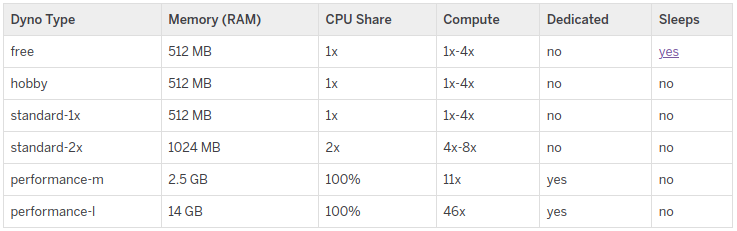
\includegraphics[width=0.9\textwidth,keepaspectratio]{dyno_types}
       	\caption{Diferentes tipos de \emph{dynos} en Heroku}
       	\label{fig:dyno_types}
    \end{figure}
    
    FirstMarket ha sido desplegada en Heroku usando un \emph{dyno} del tipo \emph{hobby} con configuración \emph{web}. En la figura \ref{fig:heroku} se muestra el panel central desde donde se gestiona el despliegue.
    
    \begin{figure}[hbt!]
       	\centering
       	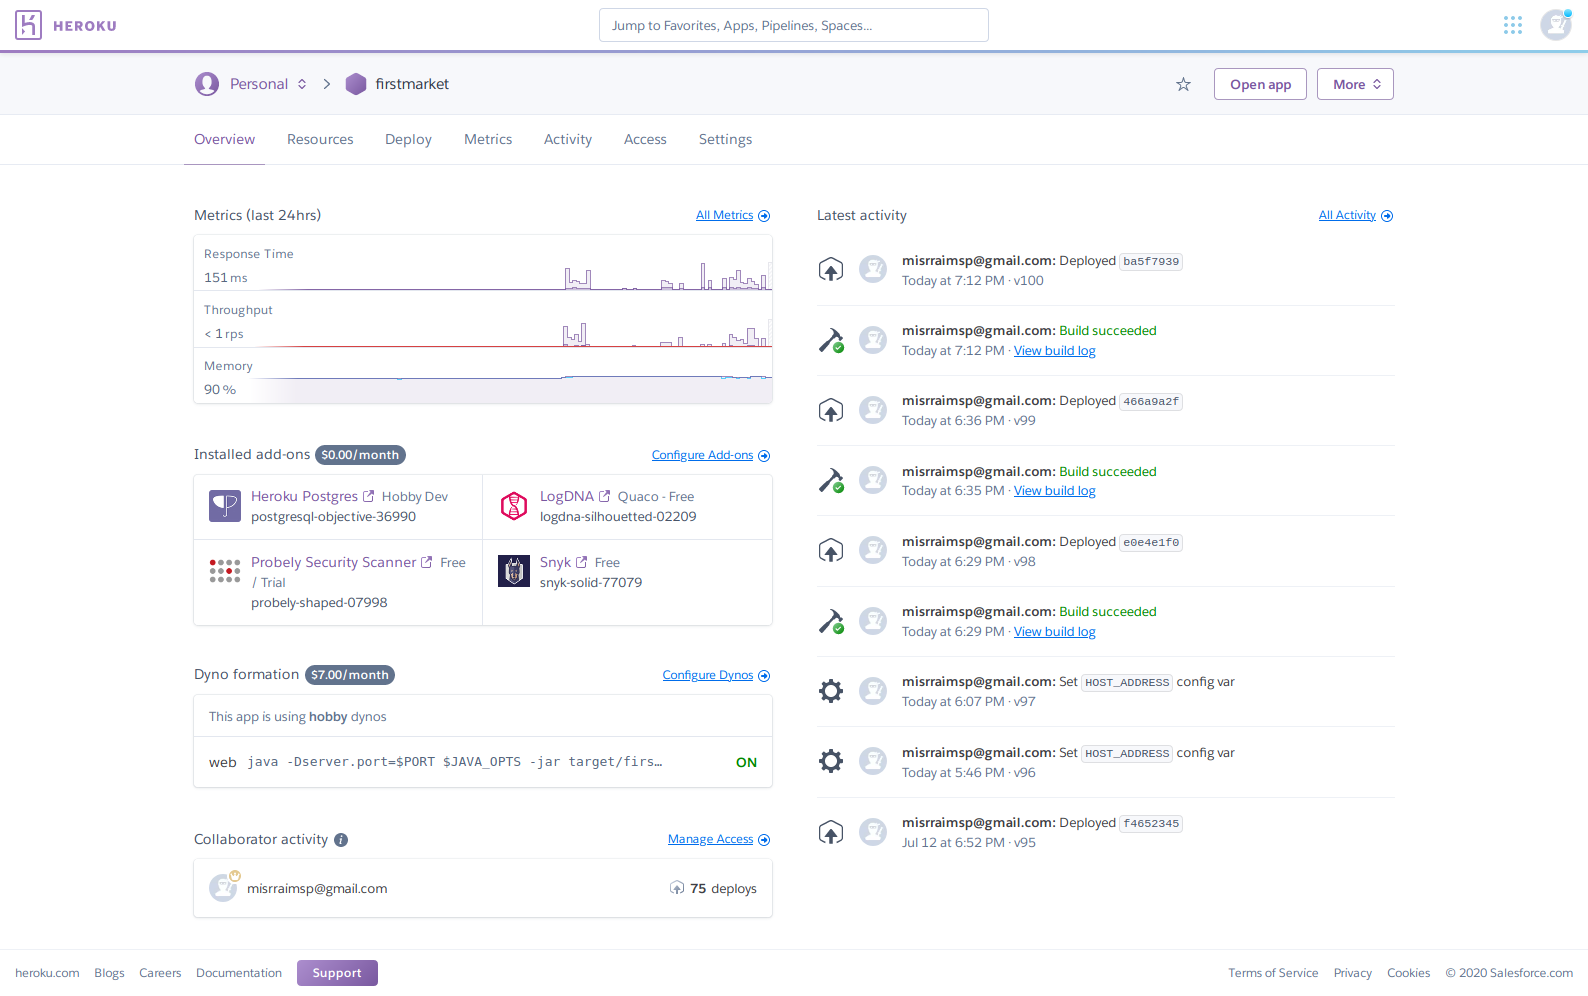
\includegraphics[width=\textwidth,keepaspectratio]{heroku}
       	\caption{Panel de control del despliegue de FirstMarket en Heroku}
       	\label{fig:heroku}
    \end{figure}

    \subsection{Heroku Add-ons} \label{sec:addons}
    Un aspecto interesante de Heroku es su oferta de \emph{Add-ons}, accesible en su \href{https://elements.heroku.com/addons}{marketplace}. Se trata de módulos que se pueden añadir a la aplicación web, algunos gratuitos y otros de pago. La aplicación web desarrollada hace uso de los siguientes:
    
    \begin{itemize}
       	\item[-] \href{https://elements.heroku.com/addons/heroku-postgresql}{Heroku Postgres}. Este es el servicio de base de datos utilizado para la capa de persistencia de la aplicación web cuando está desplegada en Heroku. El plan contratado es el gratuito, estando restringido a que el total de filas en la base de datos no supere las 10000, y con un máximo de 20 conexiones disponibles. En la figura \ref{fig:herokupostgres} se muestra el panel central de este servicio. Destacar la posibilidad de crear \emph{Dataclips}, que son consultas almacenadas sobre la base de datos. Como se aprecia, el número de filas se encuentra por debajo del límite.
       	
       	\begin{figure}[hbt!]
       		\centering
       		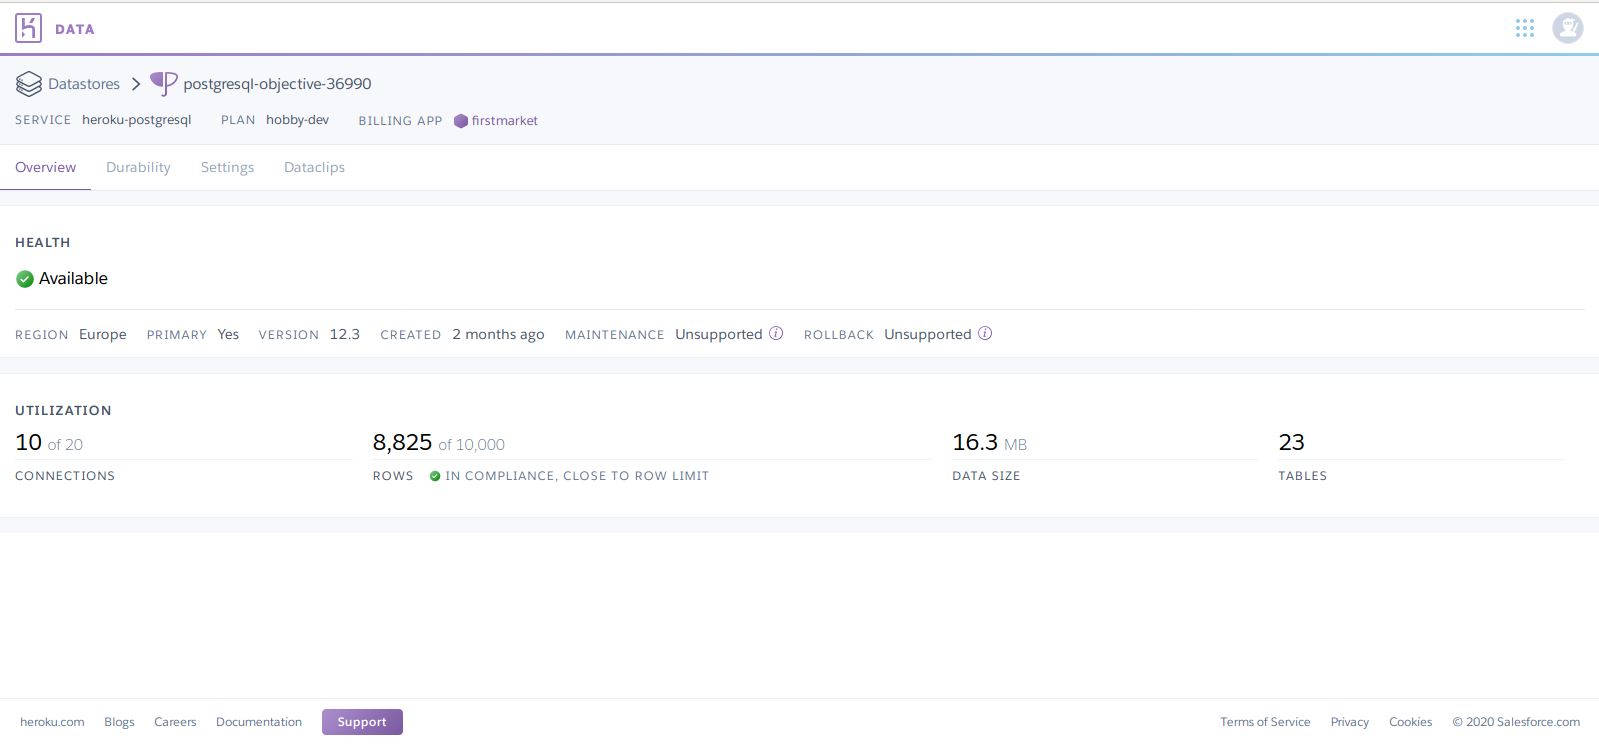
\includegraphics[width=\textwidth,keepaspectratio]{herokupostgres}
       		\caption{Panel de control de Heroku Postgres}
       		\label{fig:herokupostgres}
       	\end{figure}
       	
       	\item[-] \href{https://elements.heroku.com/addons/logdna}{LogDNA}. Este servicio permite acceder a los registros emitidos, tanto por la Heroku como por la aplicación web, de una manera sencilla a través del navegador. Tiene multitud de opciones de configuración, siendo la interfaz gráfica la mostrada en la figura \ref{fig:logdna}.
       	
       	\begin{figure}[hbt!]
       		\centering
       		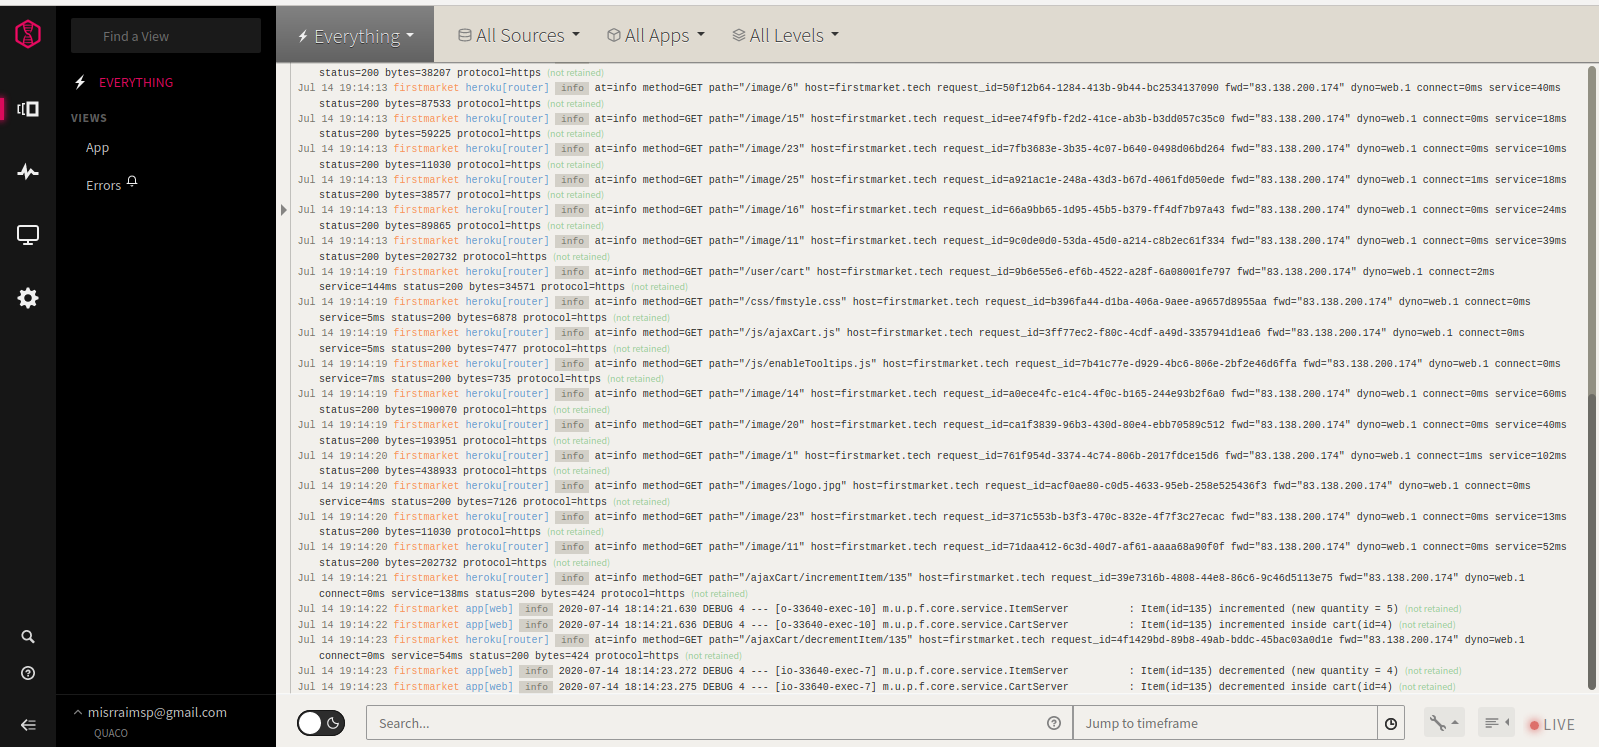
\includegraphics[width=\textwidth,keepaspectratio]{logdna}
       		\caption{Registros con LogDNA}
       		\label{fig:logdna}
       	\end{figure}
       	
       	\item[-] \href{https://elements.heroku.com/addons/probely}{Probely}. Este es un servicio de detección de vulnerabilidades de seguridad. En su versión pro, a la cual se ha tenido acceso gratuito durante dos semanas, permite realizar multitud de pruebas a la aplicación web, generando un informe de forma automática con los problemas encontrados y sus posibles soluciones. Se evaluó la aplicación web desarrollada con dos test diferentes: un análisis en profundidad estándar de Probely y un análisis OWASP top 10. Los resultados son comentados en la sección \ref{sec:vulnerabilities}.
       	\item[-] \href{https://elements.heroku.com/addons/snyk}{Snyk}. Este add-on revisa las dependencias del proyecto en busca de vulnerabilidades de seguridad conocidas. En su versión gratuita permite realizar hasta 200 test al mes, pero no emite informes es formato pdf. Los resultados son comentados en la sección \ref{sec:vulnerabilities}.
    \end{itemize}

	\subsection{firstmarket.tech}
	Por defecto, Heroku muestra sus aplicaciones web en el dominio \emph{nombre\_aplicacion.herokuapp.com}, aunque permite de forma sencilla y sin coste adicional \href{https://devcenter.heroku.com/articles/custom-domains}{añadir otros dominios}. Así, para la apertura al público de FirstMarket se ha comprado el dominio \textbf{\emph{firstmarket.tech}}, a través del registrador de dominios \href{https://www.namecheap.com/}{namecheap}.
	
	Una vez adquirido el dominio, se debe configurar sus registros DNS para que apunten a Heroku, que es donde se está ejecutando la aplicación. La figura \ref{fig:dns} muestra dichos registros DNS configurados en el panel de control que ofrece namecheap.
	
	\begin{figure}[hbt!]
		\centering
		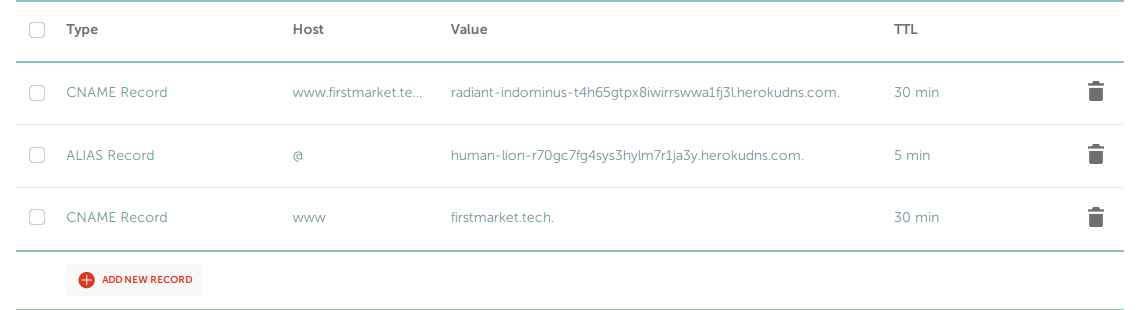
\includegraphics[width=\textwidth,keepaspectratio]{dns}
		\caption{Configuración de los registros DNS de firstmarket.tech en namecheap}
		\label{fig:dns}
	\end{figure}

	\section{Seguridad}
	La palabra seguridad es empleada en multitud de situaciones dentro del mundo de las tecnologías de la información, normalmente con significados dispares. No obstante, generalizando lo suficiente, viene a referirse a la protección que se debe proporcionar a determinados recursos, por su valor y/o sensibilidad, frente a posibles usos malintencionados.
	
	Esta sección está dedicada a las cuestiones de seguridad, en sentido amplio, relacionadas con \href{https://firstmarket.tech}{FirstMarket}.
	\subsection{HTTPS} \label{sec:https}
	Como se ha comentado, una de los principales retos que afronta el comercio electrónico es la generación de confianza. Los usuarios demandan seguridad a la hora de realizar sus compras por la red. En este sentido, el desarrollo de protocolos seguros de comunicación ha jugado un papel protagonista en el rápido incremento que el comercio \emph{online} ha vivido en las últimas décadas.
	
	HTTPS, la extensión segura de HTTP, es el protocolo de comunicación segura por excelencia en la actualidad. Los datos enviados con HTTPS son protegidos mediante el protocolo Transport Layer Security (TLS), el cual brinda tres tipos de protección:
	
		\begin{itemize}
			\item[-] Privacidad. Los datos son encriptados antes de moverse por la red, de forma que nadie ajeno a la conversación pueda comprender su semántica.
			\item[-] Integridad. De una manera similar a como Git detecta los cambios en los documentos que gestiona, TLS calcula determinados parámetros criptográficos que hacen extremadamente difícil que los datos sean alterados en su camino por la red, ya sea accidental o intencionadamente, sin que el protocolo lo detecte.
			\item[-] Autenticidad. Aún teniendo garantizado que nadie podrá entender los datos enviados, y que nadie los podrá alterar sin notarse, persiste la duda de si se está comunicando con el interlocutor pretendido. Esto es, cuando alguien accede a www.firstmarket.tech debe tener la certeza de que efectivamente está intercambiando información con FirstMarket (hipotética persona jurídica). Para esta labor TLS hace uso de los certificados digitales, que un tercer agente \emph{de confianza} emite garantizando que la web de FirstMarket es www.firstmarket.tech. Este agente es el conocido en la industria como \emph{Certificate Authority} (CA). Pero, ¿quién establece la autoridad de este CA, es decir, quién asegura que es \emph{de confianza}? Otro CA, de mayor autoridad, y así sucesivamente. Esto crea una cadena de confianza, finita, englobada dentro de la \emph{Public Key Infrastructure} (PKI), la tecnología fundamental de Internet para construir la confianza acerca de la autenticidad de los agentes en la red.
		\end{itemize}
	
	La aplicación web desarrollada puede usar HTTPS, ya que por defecto este es el protocolo que Heroku proporciona para la comunicación de sus aplicaciones ejecutadas con \emph{dynos} de pago (como es el caso). En concreto, por defecto y sin coste añadido, Heroku gestiona los certificados digitales de las aplicaciones automáticamente con su servicio \href{https://devcenter.heroku.com/articles/automated-certificate-management}{\emph{Automated Certificate Management}} (ACM). Por su parte, ACM utiliza \href{https://letsencrypt.org/}{\emph{Let’s Encrypt}}, un CA abierto, gratuito y automatizado que ofrece para el bien común el \href{https://www.abetterinternet.org/}{\emph{Internet Security Research Group}}.
	
	Para finalizar, resaltar que www.firstmarket.tech impone el uso de HTTPS, es decir, los intentos de comunicarse con la aplicación web por medio de HTTP son redirigidos al uso de la versión segura. Esto se ha implementado con Spring Security, como se muestra en el listado \ref{list:https}, donde se detalla el fragmento del método \emph{configure} que especifica este comportamiento.
	\\
	
	\begin{lstlisting}[caption=Configuración de Spring Security para imponer el uso de HTTPS,label=list:https]
	@Override
	protected void configure(HttpSecurity httpSecurity) throws Exception {
		httpSecurity
			//...
			.and()
			.requiresChannel()
			.antMatchers("/**")
			.requiresSecure()
			//...
		;
	}
	\end{lstlisting}
	
	\subsection{Spring Security} \label{sec:springsec}
	Un enfoque comúnmente empleado, en el ámbito de la seguridad de la información, se basa en considerar los sistemas complejos como un conjunto de capas de abstracción, aplicándose los mecanismos de seguridad apropiados para cada una de ellas.
	
	Si se piensa en la aplicación de comercio electrónico que se ha desarrollado, esta puede modelarse en esencia como un proceso que se ejecuta en el contexto de un sistema operativo, en el seno a su vez de una máquina, la cual se comunica con otras haciendo uso de la infraestructura de Internet. Este modelo simple ya es capaz de hacer contraste entre la aplicación, el sistema operativo, la máquina y la red. Cada una de estas capas implementa sus propias medidas destinadas a proteger la información que maneja.
	
	A nivel de aplicación, los conceptos de autenticación y autorización (o acceso) son nucleares en su ámbito de seguridad. Autenticación hace referencia a la capacidad de la aplicación para identificar al usuario. Es decir, desde el punto de vista de la aplicación, responde a la pregunta ¿quién me está usando? Autorización, por su parte, refleja la capacidad de la aplicación de permitir, o denegar, el acceso a un recurso o funcionalidad de la aplicación a un determinado usuario. Como puede notarse, para que la aplicación pueda \emph{autorizar} a un usuario, debe primero \emph{autenticar} a dicho usuario.
	
	Spring Security es la piedra angular de la seguridad a nivel de aplicación del portal de comercio electrónico desarrollado, integrando las funcionalidades de autenticación y autorización encima de las características propias de Spring Framework. Además, como se verá, también ofrece mecanismos de protección frente a multitud de vulnerabilidades comunes a nivel de aplicación.
	
	\subsubsection{FilterChain}
	Como se comenta en la sección \ref{sec:spring}, las aplicaciones web con Spring basadas en el stack servlet, como es el caso, siguen el patrón \emph{front controller}, en el que el servlet \href{https://docs.spring.io/spring/docs/current/spring-framework-reference/web.html#mvc-servlet}{\emph{DispatcherServlet}} ejerce de punto de entrada y distribuidor de las peticiones HTTP hacia los \emph{@Controller}/\emph{@RestController} adecuados.
	
	El \emph{DispatcherServlet} no integra lógica de autenticación/autorización, por lo que, en ausencia de alternativas, esta debería ser implementada en las clases \emph{@Controller}/\emph{@RestController} en las que delega las peticiones HTTP. Esto, por supuesto, destrozaría el principio de separación de responsabilidades. 
	
	Afortunadamente, sí que existe alternativa, los Java \href{https://www.oracle.com/java/technologies/filters.html}{Filters}. Estos componentes interceptan el tráfico entrante y/o saliente de los servlets, permitiendo inyectar la lógica que se desee. Así, la autenticación/autorización puede ser implementada en estos \emph{filters}, de forma que las labores de seguridad sean llevadas a cabo antes de que las peticiones HTTP alcancen el \emph{DispatcherServlet}.
	
	Además, los \emph{filters} poseen la capacidad de concatenarse entre sí, creando un \emph{filter chain} o cadena de filtros, como se muestra en la figura \ref{fig:filterchain}, tomada de la documentación oficial de Spring Security. Esto permite, otra vez, separar responsabilidades, e insertar en cada filtro la lógica de una funcionalidad concreta.
	
	\begin{figure}[hbt!]
		\centering
		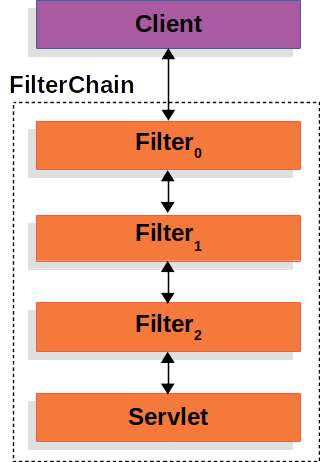
\includegraphics[width=0.4\textwidth,keepaspectratio]{filterchain}
		\caption{Encadenamiento de filtros}
		\label{fig:filterchain}
	\end{figure}
	
	Por ejemplo, una petición HTTP podría primero alcanzar un filtro destinado a recabar las credenciales de autenticación del usuario (por ejemplo un formulario de \emph{login}). Después, con dichas credenciales, atravesar el filtro que las comprueba, y autenticar así o no al usuario. Seguidamente podría estar el filtro que decide si el usuario recién autenticado posee el permiso necesario para acceder al recurso o funcionalidad pedida. Por último, en caso necesario, la petición HTTP llegaría al \emph{DispatcherServlet}.
	
	En el listado \ref{list:filter_chain} se aprecia el mensaje de registro emitido durante el arranque de la aplicación en el que se detalla la cadena de filtros que Spring Security proporciona. Pues bien, en esencia, \textbf{Spring Security \emph{es} esta concatenación de filtros} antes del \emph{DispatcherServlet}. 
	\\
	
	\begin{lstlisting}[caption=Cadena de filtros creada por Spring Security, label=list:filter_chain]
	2020-07-18 17:20:19.718  DefaultSecurityFilterChain: 
	Creating filter chain: any request, 
	[
	ChannelProcessingFilter, 
	WebAsyncManagerIntegrationFilter, 
	SecurityContextPersistenceFilter, 
	HeaderWriterFilter, 
	CsrfFilter, 
	LogoutFilter, 
	UsernamePasswordAuthenticationFilter, 
	RequestCacheAwareFilter, 
	SecurityContextHolderAwareRequestFilter, 
	AnonymousAuthenticationFilter, 
	SessionManagementFilter, 
	ExceptionTranslationFilter, 
	FilterSecurityInterceptor
	]
	\end{lstlisting}
	
	\subsubsection{Configuración}
	En estos filtros Spring Security implementa la autenticación/autorización y la protección frente a determinados tipos de ataques. Lo que resta es configurarlos para satisfacer las necesidades propias de cada aplicación. Esta configuración se lleva a cabo extendiendo la clase de Spring Security \emph{WebSecurityConfigurerAdapter} y sobreescribiendo su método \emph{configure(HttpSecurity)} (expuesto en el listado \ref{list:springsec_config}), tarea que en la aplicación web desarrollada realiza la clase \emph{SecurityConfig}.
	\\
	
	\begin{lstlisting}[caption=Configuración de Spring Security en FirstMarket, label=list:springsec_config]
	@Override
	protected void configure(HttpSecurity httpSecurity) throws Exception {
		httpSecurity
			// authenticate through login form
			.formLogin()
			.loginPage("/login")
			// handler for brute-force authentication prevention
			.failureHandler(customAuthenticationFailureHandler())
			
			// set logout page
			.and()
			.logout()
			.logoutSuccessUrl("/home")
			
			// authorization
			.and()
			.authorizeRequests()
			// protect role_admin resources
			.antMatchers("/admin/**")
			.access("hasRole('ROLE_ADMIN')")
			// protect role_user resources
			.antMatchers("/user/**")
			.access("hasRole('ROLE_USER')")
			// publicly open
			.antMatchers("/", "/home", "/login", "/newUser")
			.access("permitAll")
			
			// force HTTPS always
			.and()
			.requiresChannel()
			.antMatchers("/**")
			.requiresSecure()
			
			// enable csrf protection
			.and()
			.csrf()
			.ignoringAntMatchers("/listener") // open for stripe
			
			// always create new session
			.and()
			.sessionManagement()
			.sessionCreationPolicy(SessionCreationPolicy.ALWAYS)
			
			.and()
			.headers(headers -> headers
				// HTTP Strict Transport Security
				.httpStrictTransportSecurity(hsts -> hsts
					.includeSubDomains(true)
					.preload(true)
					.maxAgeInSeconds(31536000)
				)
				// Content Security Policy
				.contentSecurityPolicy(csp -> csp
					.policyDirectives("default-src 'self' https://*.stripe.com" +
						"; " +
						"script-src 'self' 'unsafe-inline' " +
						"https://*.stripe.com " +
						"https://*.fontawesome.com " +
						"https://maxcdn.bootstrapcdn.com " +
						"https://cdnjs.cloudflare.com " +
						"https://ajax.googleapis.com" +
						";" +
						"style-src 'self' 'unsafe-inline' " +
						"https://cdn.jsdelivr.net " +
						"https://maxcdn.bootstrapcdn.com " +
						"https://fonts.googleapis.com " +
						"https://*.fontawesome.com" +
						"; " +
						"font-src 'self' " +
						"https://fonts.gstatic.com " +
						"https://*.fontawesome.com" +
						"; " +
						"img-src 'self' data:"
					)
				)
				// Referrer Policy
				.referrerPolicy(referrer -> referrer
					.policy(ReferrerPolicyHeaderWriter.ReferrerPolicy.STRICT_ORIGIN)
				)
			)
		;
	}
	\end{lstlisting}
	
	\subsubsection{Autenticación}
	Spring Security ofrece toda una gama de métodos de autenticación. El usado en FirstMarket, especificado en las líneas 5 y 6 del listado \ref{list:springsec_config}, ha sido a través de un formulario, contenido en la vista \emph{login.html}, en el que el usuario introduce su dirección de correo electrónico y su contraseña.
	
	Es importante resaltar que, con el fin de garantizar la seguridad de la información de los usuarios, la aplicación web desarrollada almacena las constraseñas en la base de datos encriptadas.  En concreto, se usa el agoritmo \href{https://en.wikipedia.org/wiki/Bcrypt}{Bcrypt}. De esta forma, para saber si la contraseña es correcta, la aplicación web encripta la contraseña enviada en el formulario y la compara con la que tiene almacenada.
	
	Además, Spring Security permite especificar la lógica tras un \emph{logout}, que en el caso de la presente aplicación es simplemente una redirección a la páquina de inicio, como se muestra en las líneas 12 y 13 del listado \ref{list:springsec_config}.

	\subsubsection{Autorización}
	Como se puede apreciar en el listado \ref{list:springsec_config}, líneas de la 15 a la 26, FirstMarket implementa tres tipos de recursos: 
	
	\begin{itemize}
		\item[-] Los que sólo pueden ser accedidos por los usuarios con rol \emph{ROLE\_ADMIN}, ubicados en \emph{\nolinkurl{~/admin/**}}.
		\item[-] Los que sólo pueden ser accedidos por los usuarios con rol \emph{ROLE\_USER}, ubicados en \emph{\nolinkurl{~/user/**}}.
		\item[-] El resto, que puede ser accedido por cualquiera.
	\end{itemize}

	Notar que los dos primeros tipos requieren necesariamente autenticación previa.
	
	\subsubsection{Cross-Site Request Forgery}
	\href{https://en.wikipedia.org/wiki/Cross-site_request_forgery}{\emph{Cross-Site Request Forgery}} representa un tipo de ataque que toma ventaja de la confianza que un determinado sitio web tiene en un cliente, por ejemplo porque previamente se ha autenticado. Así, el cliente envía (sin saberlo) una petición (maliciosa) al sitio web y este la acepta dada la confianza que deposita en el primero. Es el caso inverso a los ataques \href{https://owasp.org/www-community/attacks/xss/}{\emph{Cross-Site Scripting}}, donde se saca partido de la confianza que el cliente tiene en el sitio web, ejecutando el código (malicioso) que este le envía (sin saberlo).
	
	Imagínese que un usuario se encuentra, autenticado, en la aplicación web de su banco, en la vista que le permite transferir fondos de su cuenta a otra. Esta vista, por ejemplo, mostraría un formulario como el mostrado en el listado \ref{list:csrf_form}. Al completarlo y presionar \emph{Transfer} se enviaría al servidor del banco la petición HTTP mostrada en el listado \ref{list:csrf_http}.
	\\
	
	\begin{lstlisting}[caption=Formulario inseguro para la transferencia de fondos,label=list:csrf_form]
	<form method="post" action="/transfer">
		<input type="text" name="amount"/>
		<input type="text" name="account"/>
		<input type="submit" value="Transfer"/>
	</form>
	\end{lstlisting}
	
	\begin{lstlisting}[caption=Petición HTTP insegura para la transferencia de fondos,label=list:csrf_http]
	POST /transfer HTTP/1.1
	Host: bank.example.com
	Cookie: JSESSIONID=randomid
	Content-Type: application/x-www-form-urlencoded
	
	amount=100.00&account=9876
	\end{lstlisting}
	
	Hasta aquí todo normal, pero imagínese que, antes de realizar \emph{logout} en la aplicación del banco, se visita otro sitio web, el cual sirve al cliente el formulario mostrado en el listado \ref{list:csrf_form_evil}. Si en esta situación el usuario presiona \emph{Win Money!} se enviará al servidor una petición HTTP exactamente igual que la mostrada en el listado \ref{list:csrf_http}, salvo el número de cuenta a donde se envía el dinero. Es decir, el usuario habrá sido estafado.
	\\
	
	\begin{lstlisting}[caption=Formulario para la transferencia ilegítima de fondos,label=list:csrf_form_evil]
	<form method="post" action="https://bank.example.com/transfer">
		<input type="hidden" name="amount" value="100.00"/>
		<input type="hidden" name="account" value="evilAccountNum"/>
		<input type="submit" value="Win Money!"/>
	</form>
	\end{lstlisting}
	
	El banco no tiene posibilidad de distinguir si alguna de las dos peticiones es ilegítima, ya que en ambas cree que las está haciendo el usuario autorizado para ello. ¿Por qué? porque el medio que utiliza para identificar al usuario, la \emph{cookie} de la línea 3 del listado \ref{list:csrf_http}, es exactamente igual en ambas peticiones, ya que el navegador por defecto adjunta las cookies en todas las peticiones.
	
	La manera más extendida de solucionar este problema, que Spring Security implementa por defecto, es adjuntar una pieza de información extra (\emph{token}) que sólo conozca el usuario legítimo. Obviamente, este \emph{token} no puede ser colocado en una \emph{cookie}, porque se estaría en la misma situación vulnerable anteriormente descrita. En este sentido, existen diversas alternativas de lugares donde colocar el \emph{token}, siendo en un campo oculto (llamado \emph{\_csrf}) la utilizada por defecto en Spring Security. Así, el formulario que el banco enviaría ahora al usuario sería como el mostrado en el listado \ref{list:csrf_form_token}, mientras que la petición HTTP sería la mostrada en el listado \ref{list:csrf_http_token}.
	\\
	
	\begin{lstlisting}[caption=Formulario seguro para la transferencia de fondos,label=list:csrf_form_token]
	<form method="post" action="/transfer">
		<input type="hidden" name="_csrf" value="4bfd1575-3ad1-4d21-96c7-4ef2d9f86721"/>
		<input type="text" name="amount"/>
		<input type="hidden" name="account"/>
		<input type="submit" value="Transfer"/>
	</form>
	\end{lstlisting}
	
	\begin{lstlisting}[caption=Petición HTTP segura para la transferencia de fondos,label=list:csrf_http_token]
	 POST /transfer HTTP/1.1
	Host: bank.example.com
	Cookie: JSESSIONID=randomid
	Content-Type: application/x-www-form-urlencoded
	
	amount=100.00&account=9876&_csrf=4bfd1575-3ad1-4d21-96c7- 4ef2d9f86721
	\end{lstlisting}
	
	De esta forma, el agente malintencionado ya no podrá tener acceso a la información necesaria para suplantar la identidad del usuario legítimo, teniendo ahora el banco un mecanismo para distinguirlos.
	
	Como se ha dicho, esta funcionalidad se implementa por defecto con Spring Security. Sin embargo, como se aprecia en las líneas 34 a 37 del listado \ref{list:springsec_config}, se ha modificado ligeramente el comportamiento por defecto para permitir que desde Stripe se realicen peticiones POST sin necesidad de contar con el token \emph{\_csrf}.
	
	\subsubsection[Encabezados HTTP]{Encabezados de Seguridad en las Respuestas HTTP}
	Los principales navegadores web implementan diversos controles de seguridad que entran en acción cuando desde el servidor se les especifica la configuración deseada. Los \href{https://owasp.org/www-project-secure-headers/}{encabezados de seguridad} insertados en las respuestas HTTP cumplen este papel. Esto es, son directrices que los servidores proporcionan a los clientes web, con el objetivo de establecer la configuración de la política de seguridad que se desea que el navegador implemente.
	
	\paragraph{Cache Control}
	Por defecto, Spring Security instruye al navegador, por medio de las cabeceras de respuesta mostradas en el listado \ref{list:cache_control}, para que no guarde en su caché ninguna información, debido al riesgo que esto representa para el usuario. Piénsese, por ejemplo, en una situación en la que un usuario, tras autenticarse, consulta información confidencial, que el navegador almacena en caché. Después, tras cerrar su sesión, otro usuario podría tener acceso a dicha información privada sin más que consultar las páginas guardadas en el historial de navegación.
	\\
	
	\begin{lstlisting}[caption=Cabeceras para impedir el almacenamiento en caché, label=list:cache_control]
	Cache-Control: no-cache, no-store, max-age=0, must-revalidate 
	Pragma: no-cache
	Expires: 0
	\end{lstlisting}
	
	No obstante, para el contenido estático (principalmente hojas de estilo y código JavaScript), sí se ha permitido al navegador almacenarlo en su caché, con el fin de mejorar el tiempo de carga de las páginas y ganar en experiencia de usuario, sin merma de seguridad.

	\paragraph{Content Type Options}
	Normalmente, cuando el campo \emph{content type} (tipo de contenido) no es especificado, los navegadores tratan de deducirlo para mejorar la experiencia de usuario. Por ejemplo, si el navegador encuentra un archivo JavaScript sin el tipo de contenido especificado, intentará deducir su naturaleza a partir del propio contenido y, en caso de que finalmente lo juzgue como código JS, lo ejecutará. A este procedimiento de inferencia del tipo de contenido se le conoce como \href{https://en.wikipedia.org/wiki/Content_sniffing}{\emph{content sniffing}}
	
	Este sistema de inferencia del tipo de contenido presenta el problema de ser un vector para ataques XSS (\href{https://owasp.org/www-community/attacks/xss/}{\emph{cross-site scripting}}). En efecto, existen archivos contruidos de tal manera que pueden ser interpretados de varias formas al mismo tiempo. Por ejemplo, una aplicación web puede permitir a los usuarios enviar un documento PostScript válido para posteriormente visualizarlo. Un usuario malintencionado podría crear un documento PostScript que también sea un archivo JavaScript válido y ejecutar un ataque XSS con él.
	
	Por estas razones, la configuración que por defecto ofrece Spring Security es instruir al navegador para que no realice \emph{content sniffing}, a través de la cabecera mostrada en el listado \ref{list:content_sniffing}. Notar que, como contraparte, ahora en todo momento se debe indicar el tipo de contenido en lo que se envíe al navegador para que funcione correctamente.
	\\
	
	\begin{lstlisting}[caption=Cabecera para impedir el \emph{content sniffing}, label=list:content_sniffing]
	X-Content-Type-Options: nosniff
	\end{lstlisting}
	
	\paragraph{HTTP Strict Transport Security}
	Cuando un usuario teclea la dirección web del sitio que pretende visitar, normalmente no especifica que la comunicación se haga a través de HTTPS. Es decir, se suele escribir sólo \emph{firstmarket.tech} en lugar de \emph{https://firstmarket.tech}. Esto representa un riesgo, ya que las comunicaciones HTTP son vulnerables a ataques \href{https://en.wikipedia.org/wiki/Man-in-the-middle_attack}{\emph{man in the middle}}. Es más, aunque la comunicación HTTP sea redirigida a usar la versión segura (como es el caso en la aplicación web desarollada), la vulnerabilidad comentada persistiría entre la comunicación inicial con HTTP y la redirección.
	
	Para gestionar esta situación se creó el \href{https://tools.ietf.org/html/rfc6797}{HTTP Strict Transport Security (HSTS)}, un mecanismo para que los sitios web puedan declararse como \emph{HTST host}, esto es, como accesibles únicamente mediante conexiones seguras.
	
	Una manera de alcanzar este estatus es ingresar en la lista de dominios web \emph{preloaded} gestionada en \href{https://hstspreload.org/}{hstspreload.org}. En la figura \ref{fig:preload_list_submission_success} se muestra el mensaje tras el envío del formulario de inscripción.
	
	\begin{figure}[hbt!]
		\centering
		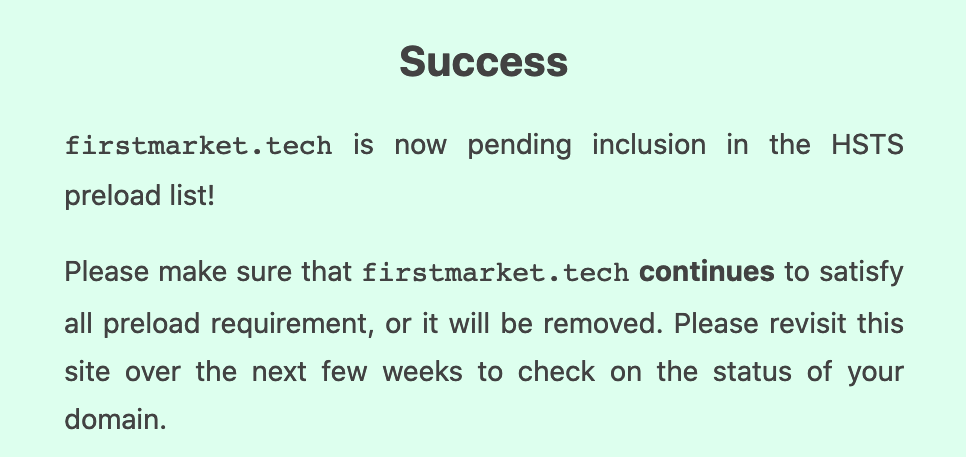
\includegraphics[width=0.7\textwidth,keepaspectratio]{preload_list_submission_success}
		\caption{Candidatura para la inclusión en la lista de dominios web \emph{preloaded}}
		\label{fig:preload_list_submission_success}
	\end{figure}
	
	Otra forma es incluyendo el encabezado \emph{Strict-Transport-Security} en las respuestas HTTP. En las líneas de la 46 a la 51 del listado \ref{list:springsec_config} se muestra la configuración realizada en Spring Security para incluir la cabecera mostrada en el listado \ref{list:hsts} en las respuestas HTTP.
	\\
	
	\begin{lstlisting}[caption=Cabecera de declaración \emph{HSTS host}, label=list:hsts]
	 Strict-Transport-Security: max-age=31536000 ; includeSubDomains ; preload
	\end{lstlisting}
	
	\paragraph{X-Frame-Options}
	Con el objetivo de prevenir los ataques conocidos como \href{https://en.wikipedia.org/wiki/Clickjacking}{\emph{clickjacking}}, Spring Security inhabilita el renderizado de vistas que contengan etiquetas HTML5 \emph{iframe}. Esto se consigue enviando a los navegadores el encabezado que se muestra en el listado \ref{list:iframe}.
	\\
	
	\begin{lstlisting}[caption=Cabecera que inhibe el uso de las etiquetas \emph{iframe}, label=list:iframe]
	 X-Frame-Options: DENY
	\end{lstlisting}
	
	\paragraph{X-XSS-Protection}
	Muchos navegadores implementan filtros anti-\href{https://owasp.org/www-community/attacks/xss/}{XSS}. Aún no representando una solución infalible al problema, ayudan mucho a su mitigación. Normalmente estos filtros están habilitados por defecto, siendo posible configurar qué hacer en caso de un positivo (por ejemplo, intentar enmendar el contenido detectado).
	
	Spring Security, por defecto, a través del encabezado que se muestra en el listado \ref{list:filtro_xss}, activa explícitamente el filtro del navegador y lo configura para que ante un positivo bloquee el contenido.
	\\
	
	\begin{lstlisting}[caption=Cabecera que activa y configura el filtro anti-XSS del navegador, label=list:filtro_xss]
	X-XSS-Protection: 1; mode=block
	\end{lstlisting}
	
	\paragraph{Content Security Policy}
	La \href{https://developer.mozilla.org/en-US/docs/Web/HTTP/CSP}{\emph{Content Security Policy}} (CSP) es un mecanismo de protección frente a vulnerabilidades de inyección de contenido, como por ejemplo el comentado \href{https://owasp.org/www-community/attacks/xss/}{\emph{cross-site scripting}}. A través de esta funcionalidad se puede declarar y, en última instancia, informar al navegador acerca de cuáles son las fuentes autorizadas desde las cuales descargar los recursos que las vistas de la aplicación web necesita.
	
	Esta política de permisos, no trivial, depende de las necesidades de cada sitio web, y es por ello que Spring Security no la configura por defecto. Así, en el listado \ref{list:springsec_config}, entre las líneas 52 y 75, se declara la CSP de la aplicación web desarollada. Como se aprecia, se establecen los dominios desde los cuales obtener 4 tipos de recursos: los \emph{scripts}, las hojas de estilo, las fuentes y las imágenes. También se establece que todo el contenido fuera de lo explicitado sólo pueda ser obtenido desde \emph{firstmarket.tech} y desde \emph{*.stripe.com}.
	
	\paragraph{Referrer  Policy}
	Uno de los muchos encabezados que se incluyen en una petición HTTP es el \href{https://developer.mozilla.org/en-US/docs/Web/HTTP/Headers/Referer}{\emph{Referer}}, que contiene la dirección de la página web anterior desde la cual se realizó la navegación a la página actual. Por otro lado, el encabezado \href{https://developer.mozilla.org/en-US/docs/Web/HTTP/Headers/Referrer-Policy}{\emph{Referrer-Policy}} controla qué restricciones aplicar a la información suministrada en el encabezado \emph{Referer}.
	
	Es importante establecer un criterio apropiado ya que, por ejemplo, si no se especifica política alguna que restrinja la información contenida en el encabezado \emph{Referer}, este podría contener el token de seguridad que FirstMarket adjunta en el link que envía a los usuarios para verificar la dirección de correo electrónico. En general, la información sensible que puedan contener las URL quedaría expuesta en el encabezado \emph{Referer}.
	
	Spring Security permite de una manera sencilla configurar la política deseada, que en el caso de FirstMarket ha sido \textbf{\emph{strict-origin}}, como se aprecia en las líneas 76 y 79 del listado \ref{list:springsec_config}. Esta política establece que sólo se envía información en el encabezado \emph{Referer} si el destinatario usa HTTPS. Esta es la parte \emph{strict} de \emph{strict-origin}. La parte \emph{origin} significa que sólo se envía el origen de la dirección. Por ejemplo, de \emph{www.firstmarket.tech/login?error=true} sólo sería enviado \emph{www.firstmarket.tech}.
	
	\subsection{Autenticación por Fuerza Bruta}
	\subsection{Validación de Entradas}
	Por validación se entiende las comprobaciones que la aplicación web hace sobre los datos que le son proporcionados externamente. El caso más común es cuando un usuario envía un formulario cumplimentado a la aplicación web, y esta, antes de procesar la información, comprueba que se cumplen ciertas reglas. Por ejemplo, puede requerirse que el campo de email sea efectivamente una dirección de correo válida, o que la fecha de nacimiento sea una fecha pasada válida (nadie puede nacer el 30 de febrero, por ejemplo). Esto se hace para garantizar la consistencia de los datos en la base de datos y, quizás más importante, para evitar ataques de inyección de contenido.
	
	Esta comprobación se puede hacer tanto en cliente como en servidor. Desde el punto de vista de la seguridad, realizar la comprobación en servidor es \textbf{obligatorio}, ya que las comprobaciones en cliente son muy fácilmente circunvaladas. Por otro lado, desde el punto de vista de la experiencia de usuario es muy recomendable implementarla también en cliente, ya que permite al usuario tener un \emph{feedback} mucho más rápido que si debiese esperar a que el servidor responda. En definitiva, la mejor práctica es implementar la validación tanto en \emph{backend} como en \emph{frontend}, y así se ha implementado en la aplicación web desarrollada. Resaltar, además, que los componentes de validación en \emph{backend} están en el paquete \emph{util.validation}.
	
	Mucha es la información que FirstMarket debe validar, pero a grandes rasgos se puede dividir en numérica y textual. El primer grupo presenta poca dificultad, se trata de comprobar rangos de valores principalmente. Para el segundo grupo las expresiones regulares son el arma perfecta. En el archivo de configuración \emph{application.yml} se detallan las expresiones regulares y los rangos numéricos utilizados. A modo de ejemplo, la propiedad definida en este archivo de configuración que especifica la expresión regular contra la que validar las contraseñas se muestra en el listado \ref{list:regex_pw}.
	\\
	
	\begin{lstlisting}[caption=Expresión regular para las contraseñas,label=list:regex_pw]
	fm:
		validation:
			regex:
				password: ^(?=.*\d)(?=.*[a-z])(?=.*[A-Z]).{8,16}$
	\end{lstlisting}
	
	Así, esta expresión regular es utilizada por la aplicación web para comprobar, tanto en \emph{frontend} como en \emph{backend}, que cuando un usuario proporciona una nueva contraseña esta tenga una longitud de entre 8 y 16 caractéres e incluya al menos una minúscula, una mayúscula y un dígito.
	
	Existe un campo que destaca por su manera de ser validado. Se trata del ISBN (International Standard Book Number) de los libros. Este campo necesita validación en dos vertientes. La primera se realiza utilizando las ya mencionadas expresiones regulares, pero, para validar si se trata de un ISBN válido, aún hay que calcular el dígito de control y comprobar que coincida con el último dígito del código. Los ISBN tuvieron 10 dígitos hasta diciembre de 2006, pero desde entonces tienen siempre 13 (ambas versiones con diferentes algoritmos de cálculo del dígito de control). Así pues, la validación implementada en FirstMarket da soporte a ambos formatos de ISBN.
	
	\subsection{Stripe Radar} \label{sec:striperadar}
	\subsection{Análisis de Vulnerabilidades} \label{sec:vulnerabilities}
	Como se comentó en la sección \ref{sec:addons}, la seguridad de la aplicación web ha sido testada con la ayuda de \href{https://probely.com/}{Probely} y \href{https://snyk.io/}{Snyk}. La primera herramienta detectó 5 vulnerabilidades, mientras que la segunda 13. Del total, 14 responden a vulnerabilidades conocidas en librerías utilizadas por la aplicación web, por lo que su resolución se basa en actualizar las versiones de dichas dependencias. A continuación se pasa a comentar los problemas encontrados, haciendo especial énfasis en las 4 vulnerabilidades propias de la aplicación web desarrollada: 
	
	\begin{itemize}
		\item[-] \textbf{\emph{Reflected cross-site scripting}}. Esta vulnerabilidad, considerada de \textbf{alto riesgo}, fue encontrada durante el test OWASP top 10 realizado con Probely.
		
		Este riesgo se encuentra bastante extendido por Internet y ocurre cuando el servidor de la aplicación toma un input del cliente y lo devuelve nuevamente sin validar o codificar adecuadamente para ser mostrado por pantalla. El adjetivo \emph{reflected} proviene del código malicioso que se envía al servidor y se refleja en el navegador de la víctima en el código fuente de la página.
		
		En el caso concreto de la presente aplicación, esta vulnerabilidad se encontró en la vista de las categorías, \emph{categories.html}. En esta vista, como se explica en la sección \ref{sec:hierarchy}, el código HTML necesario para mostrar la estructura de categorías anidadas se genera dinámicamente con \emph{categoriesBuilder.js}. Para que este \emph{script} pueda realizar su función, el servidor incrusta dentro de \emph{categories.html} la información de las categorías en formato JSON.
		\\
		
		\begin{lstlisting}[caption=Extracto de categories.html con la vulnerabilidad encontrada,label=list:rcss_template]
		...
		<!-- categories dynamically generated -->
		<i id="catHolder" th:attr="jsonStringCategories=${jsonStringCategories}"></i>
		<!-- insecure: reflected XSS
		<script th:utext="'let jsonStringCats = \'' + ${jsonStringCategories} + '\';'"></script>
		-->
		<script th:src="@{/js/categoriesBuilder.js}"></script>
		...
		\end{lstlisting}
		
		Como se aprecia en la línea 5 del listado \ref{list:rcss_template}, la manera vulnerable de hacer disponible la información de categorías a \emph{categoriesBuilder.js} es haciendo uso de la directiva de Thymeleaf \textbf{\emph{th:utext}} en la declaración de la variable JavaScript \emph{jsonStringCats}, donde la \emph{u} significa \emph{unscaped}. Esta manera de renderizar la información del servidor es el origen del problema, ya que los caracteres especiales que puedan contener los nombres de las categorías no son apropiadamente codificados.
		
		Una manera segura, que resuelve el problema, es la implementada en la línea 3 del mismo listado \ref{list:rcss_template}, donde se utiliza la directiva de Thymeleaf \emph{th:attr} para incrustar la estructura JSON como un atributo HTML. Esta directiva sí codifica adecuadamente los caracteres especiales, mitigando el riesgo de insertar código malicioso en el nombre de las categorías y que sea servido y expuesto a los clientes.
		
		\begin{figure}[hbt!]
			\centering
			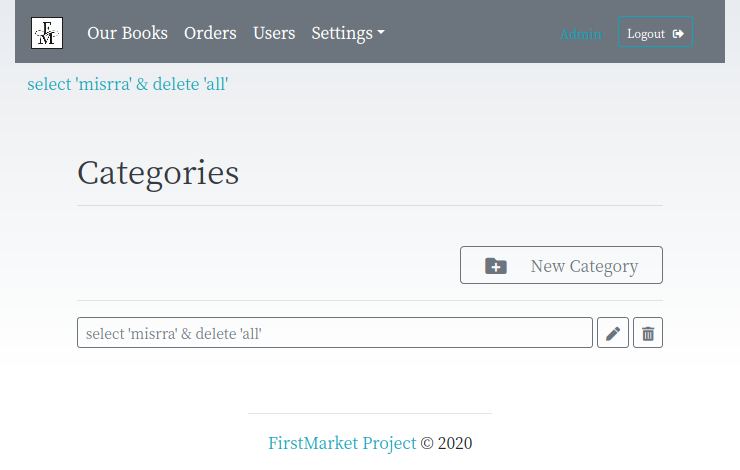
\includegraphics[width=\textwidth,keepaspectratio]{cat_rcss}
			\caption{Categoría con caracteres especiales en su nombre}
			\label{fig:cat_rcss}
		\end{figure}
		
		En la figura \ref{fig:cat_rcss} se muestra un nombre de categoría con caracteres especiales, exponiéndose en el listado \ref{list:rcss_html} un extracto de su código fuente, generado con ambos métodos: el seguro en la línea 3 y el inseguro, sin codificar los caracteres, en la línea 5.
		\\
		
		\begin{lstlisting}[caption=Extracto del HTML generado a partir del template categories.html,label=list:rcss_html]
		...
		<!-- categories dynamically generated -->
		<i id="catHolder" jsonStringCategories="{ &quot;name&quot;:&quot;firstmarket&quot;, &quot;id&quot;:6, &quot;children&quot;:[{ &quot;name&quot;:&quot;select &#39;misrra&#39; &amp; delete &#39;all&#39;&quot;, &quot;id&quot;:68, &quot;children&quot;:[]}]}"></i>
		<!-- insecure: reflected XSS 
		<script>let jsonStringCats = '{ "name":"firstmarket", "id":6, "children":[{ "name":"select 'misrra' & delete 'all'", "id":68, "children":[]}]}';</script>
		-->
		<script src="/js/categoriesBuilder.js"></script>
		...
		\end{lstlisting}
		
		\item[-] \textbf{\emph{Potential DoS on TLS Client Renegotiation}}. Esta vulnerabilidad (\href{https://nvd.nist.gov/vuln/detail/CVE-2011-1473}{CVE-2011-1473}) está basada en la asimetría de trabajo que tiene lugar cuando el cliente inicia una renegociación de los parámetros criptográficos de una conexión TLS con el servidor, soportando este la mayor carga de trabajo. Así, un cliente malicioso podría iniciar una conexión TLS y seguidamente requerir el procedimiento de renegociación repetidas veces, en busca de colmar los recursos del servidor.
		
		La renegociación para acordar nuevos parámetros de cifrado se desarrolla dentro de una única conexión TCP. Esto es clave, ya que otros ataques DoS relacionados con TLS se basan en inundar al servidor con nuevas conexiones TCP, contra lo cual muchos cortafuegos implementan algún tipo de control del ritmo de peticiones de nuevas conexiones TCP. Pero esta vulnerabilidad explota que la renegociación tiene lugar dentro de una única conexión TCP, evitando así este tipo de controles.
		
		Para controlar esta amenaza en la aplicación web desarrollada sería necesario implementar una restricción sobre el ratio de peticiones de renegociación iniciadas por el cliente, o simplemente deshabilitar esta capacidad. Se ha optado por la segunda opción, dada la sencillez de su implementación y el bajo o nulo impacto en la experiencia de usuario. Así, para deshabilitar esta opción, Java 8 introdujo una nueva variable de la JVM, de forma que únicamente es necesario invocar la aplicación con la opción detallada en el listado \ref{list:tls_renegotiation}.
		\\
		
		\begin{lstlisting}[caption=Deshabilitado del inicio por parte del cliente de la renegociación TLS,label=list:tls_renegotiation]
		-Djdk.tls.rejectClientInitiatedRenegotiation=true
		\end{lstlisting}
		
		\item[-] \textbf{\emph{Outdated TLS protocol version 1.0 supported}}. Como se explica en la sección \ref{sec:https}, Heroku ofrece conexiones seguras con TLS, por defecto, a través de su funcionalidad \href{https://devcenter.heroku.com/articles/automated-certificate-management}{\emph{Automated Certificate Management}}. La vulnerabilidad descrita en este apartado se produce por el hecho de que ACM no fuerza el uso de TLS v1.2+, es decir, no deshabilita el uso de versiones obsoletas de TLS.
		
		Tal como se explica en su \href{https://devcenter.heroku.com/articles/understanding-ssl-on-heroku#when-to-use-the-ssl-endpoint}{documentación}, para deshabilitar el soporte a las versiones inseguras, TLS v1.0 y TLS v1.1, sería necesario sustituir ACM por \href{https://devcenter.heroku.com/articles/ssl-endpoint}{SSL Endpoint}, el cual es un servicio con un coste de 20 dólares mensuales.
		
		Teniendo en cuenta el coste indicado, y la reciente (8 Jul 2020) notificación recibida desde Heroku, mostrada a seguir, se ha optado por continuar usando ACM:
		
		\begin{displayquote}
			Dear Heroku Customer,
			\\
			
			At Salesforce, our top priority is providing you with a trusted Heroku platform, and today we begin our migration off of older, less secure TLS versions with a plan to completely block TLS v1.0/v1.1 next year after July 31, 2021. [...]
			\\
			
			Heroku currently supports TLS v1.0/v1.1, as well as the latest, more secure TLS v1.2+ protocol on all apps. [...]
			\\
			
			Today, Heroku begins implementing these recommendations to transition all apps to TLS v1.2+, so that we can End of Life TLS v1.0/v1.1 next year. [...]
			\\
			
			Beginning on June 1, 2021, we will begin migration all apps to the new cipher suites and block TLS v1.0/v1.1 completing this migration by July 31, 2021. 
			\\
			
			After July 31, 2021, clients that access Heroku apps using TLS v1.0/v1.0 will be blocked. [...]
			\\
			
			Sincerely, Heroku.
		\end{displayquote}
		
		\item[-] \textbf{\emph{Referrer policy not defined}}. La vulnerabilidad comentada en este punto se debe a que no se había especificado qué política de \emph{Referer} emplear, con el consecuente riesgo de enviar información sensible en dicho encabezado. Como se explica en la sección \ref{sec:springsec}, el riesgo queda mitigado al especificar la política \emph{strict-origin} con Spring Security.
		
		\item[-] \textbf{\emph{Vulnerabilidades en librerías de terceros}}. Las restantes 14 vulnerabilidades se han solucionado por medio de actualizaciones. Por la propia naturaleza de la herramienta, todas los problemas detectados por Snyk entran dentro de este epígrafe, mostrándose en la figura \ref{fig:snyk} dos de las vulnerabilidades más graves que ha detectado. Las actualizaciones realizadas han sido las siguientes:
		
		\begin{itemize}
			\item[1.] org.springframework.boot:spring-boot $\rightarrow$ 2.3.1.RELEASE
			\item[2.] org.springframework:spring-web $\rightarrow$ 5.2.4.RELEASE
			\item[3.] org.springframework:spring-webmvc $\rightarrow$ 5.2.4.RELEASE
			\item[4.] org.hibernate:hibernate-core $\rightarrow$ 5.4.18.Final
			\item[5.] org.springframework.security:spring-security-core $\rightarrow$ 5.3.2.RELEASE
			\item[6.] org.apache.tomcat.embed:tomcat-embed-core $\rightarrow$ 9.0.37
			\item[7.] org.webjars:jquery $\rightarrow$ 3.5.1
		\end{itemize}
		
		\begin{figure}[hbt!]
			\centering
			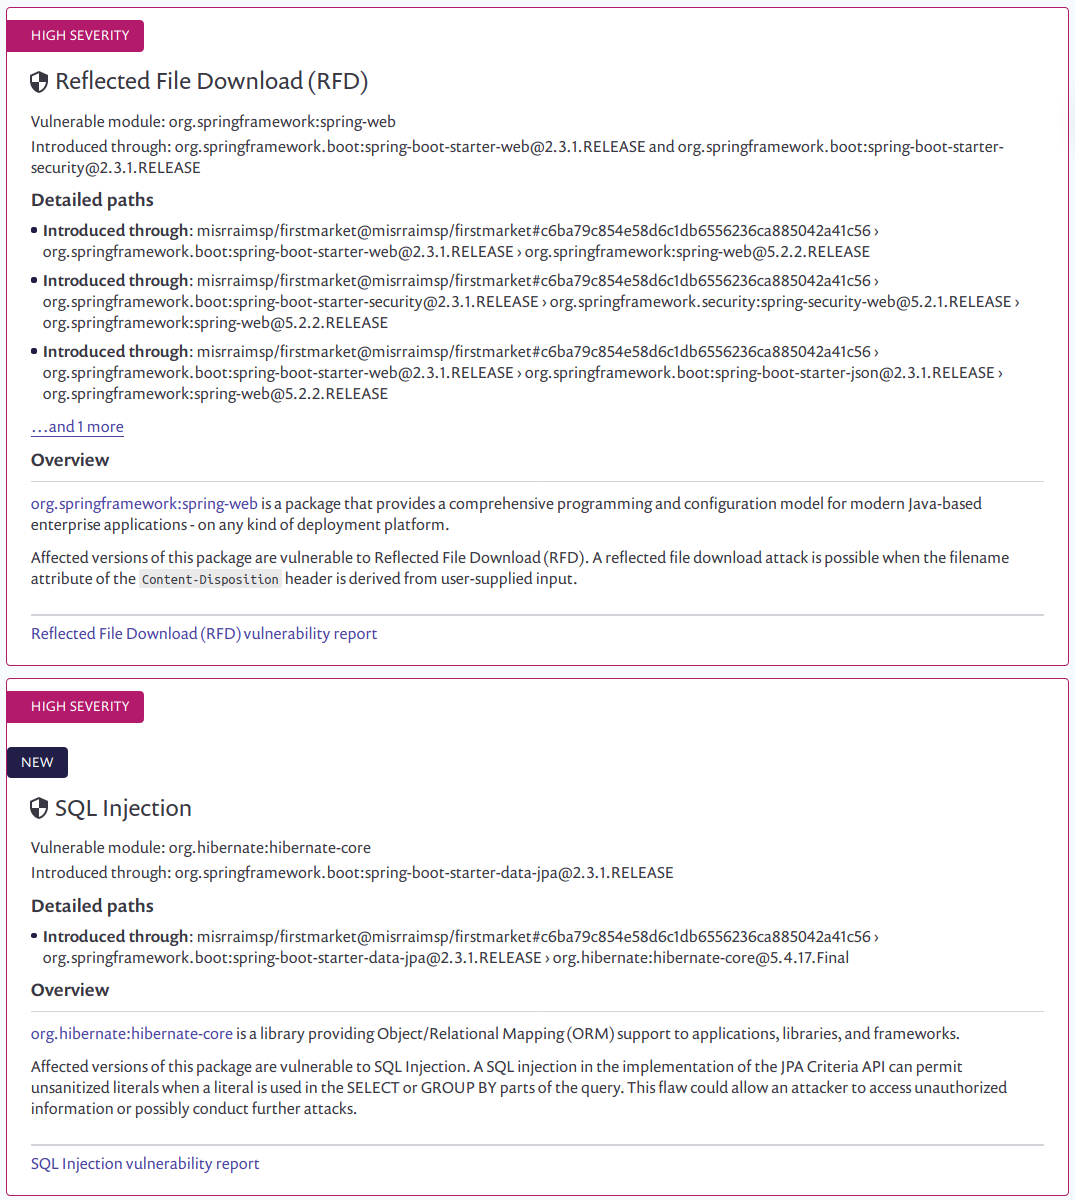
\includegraphics[width=\textwidth,keepaspectratio]{snyk}
			\caption{Ejemplo de vulnerabilidades encontradas por Snyk}
			\label{fig:snyk}
		\end{figure}
		
		Un aspecto que debe resaltarse es que las actualizaciones de la 2 a la 6, incluidas ellas, han tenido que establecerse sobrescribiendo la configuración que por defecto ofrece Spring Boot a través del fichero \emph{spring-boot-starter-parent}, del cual hereda el \emph{pom.xml} de la aplicación web desarrollada. Esto es importante porque se está saliendo del terreno seguro que esta configuración por defecto suministra, en el sentido de que desde Spring se ha testado que las versiones establecidas por defecto funcionan sin problemas de compatibilidades entre sí.
		
	
	\end{itemize}
	
	
    % MANUALES
    \section{Manuales}
    En esta seccion se va a describir las cuestiones necesarias para facilitar el uso de la aplicacion web por parte de los usuarios
        \subsection{Cliente}
    aqui va la descripcion para el usuario cliente
        \subsection{Administrador}
    aquie se describe el uso del admin

	\section{Presupuesto}
	%precio de los cursos
	%Resaltar que este \emph{dyno} tiene un coste de 7 dólares por mes.

    \section{Mejoras y Ampliaciones}
    %Testar el software
    
    %Sistema de valoracion por parte de los usuarios de los libros
    
    %STRIPE -- https://stripe.com/docs/radar/checklist
    %Using Customer objects when creating payments allows Stripe to track the payment patterns for each customer over time. This significantly increases our ability to identify irregularities in purchasing behavior. To do this, you should:
    
    %pentesting con https://www.zaproxy.org/
    


\end{document}
